\documentclass[journal]{IEEEtran}
\usepackage{amsmath,amssymb,mathtools,mathrsfs}
\usepackage{graphicx}
\usepackage{booktabs}
\usepackage{multirow}
\usepackage{array}
\usepackage[table]{xcolor}
\usepackage[hidelinks]{hyperref}
\usepackage[linesnumbered,ruled,vlined]{algorithm2e}
\usepackage{caption}
\captionsetup[figure]{name={Fig.},labelsep=period}
\graphicspath{{figures/}}
\pagestyle{plain}
\hyphenation{op-tical net-works semi-conduc-tor}

\newcommand{\method}{QA-DR-MADDPG}
\newcommand{\vect}[1]{\boldsymbol{#1}}
\newcommand{\E}{\mathbb{E}}

\begin{document}

\title{Queue-Aware Domain-Randomized Hybrid MADDPG for Multi-UAV-Assisted Vehicular Edge Computing}

\author{
\begin{tabular}[t]{c}Arpit Anand\\IIT2023170\end{tabular}\quad
\begin{tabular}[t]{c}Hridayesh\\IIT2023148\end{tabular}\quad
\begin{tabular}[t]{c}Kinshuk\\IIT2023079\end{tabular}\quad
\begin{tabular}[t]{c}Rahul Garg\\IIT2023173\end{tabular}\quad
\begin{tabular}[t]{c}Anurag Sikarwar\\IIT2023242\end{tabular}
}

\maketitle

\begin{abstract}
Vehicular edge computing with several UAVs has to decide, slot by slot, where
each task is offloaded, how radio and processor capacity are shared, and
where the UAVs fly, while traffic, harvested energy and backhaul capacity
keep changing. This report presents \method, a queue-aware,
domain-randomized form of hybrid multi-agent deep deterministic policy
gradient, for a network of vehicles, RSUs, UAVs and a cloud server. A task
is not treated as served when it is dispatched: it stays in explicit
transmission, computation and backhaul queues until all of its work is done.
These physical queues and a set of virtual energy-deficit queues make up a
Lyapunov drift-plus-penalty reward. Hard limits (battery causality, the
return reserve, airspace bounds, acceleration and UAV separation) are left to
a feasibility controller. Each agent role has its own actor for mixed
categorical and continuous actions, and the critics are centralized during
training. Instead of meta-learning an initialization, we train one policy
over seven declared operating conditions and deploy it without any online
gradient step. Frozen checkpoints from five learner seeds were evaluated in
1,750 learned-controller test runs. Compared with nominal Hybrid MADDPG,
domain randomization lifted the numerical deadline-success rate from 22.2\%
to 41.5\% and completion from 77.9\% to 82.0\%. A separate 700-run ablation
showed that weighting the physical queues adds 0.470 tasks/s of throughput
and removes 467.0 Gcycles of final backlog; for both effects the paired
95\% confidence intervals exclude zero. No learned controller violated the
modeled battery, separation or physical-feasibility constraints. The
intervals are still wide, though, so we see the results as a gain in
numerical robustness and not as general statistical superiority.
\end{abstract}

\begin{IEEEkeywords}
Vehicular edge computing, multi-UAV systems, domain randomization, MADDPG,
task queues, Lyapunov optimization, energy-aware control.
\end{IEEEkeywords}

\section{Introduction}
Cooperative perception, localization and traffic analysis all give vehicles
computation tasks with short deadlines. Many of these tasks carry a lot of
input data and need more processor cycles than a single vehicle can reliably
supply, which is where vehicular edge computing (VEC) comes in: the task can
stay on the vehicle or be handed to a nearby edge server or to the cloud.
None of these options is free. The vehicle's own processor and energy budget
are small. An RSU has more computing power but only serves vehicles inside
its region, and the cloud adds access and backhaul delay. A server that is
picked only for its advertised CPU capacity, or for a good instantaneous
radio rate, may turn out to be congested
already~\cite{liu2020uav,liang2025rav}.

UAV-mounted edge servers help in areas where fixed infrastructure is sparse
or temporarily overloaded. A UAV can change its altitude and horizontal
position to get a better link and to move closer to a cluster of vehicles,
but moving costs energy. Propulsion is usually a large part of a UAV's
consumption, and reception, backhaul transmission and onboard computing are
paid from the same battery~\cite{liu2020uav,talukdar2026mappo}. Flying to
improve the current uplink may leave less energy for tasks that arrive later,
or too little for a safe return. In our formulation, offloading, processor
allocation, backhaul use and 3-D flight are therefore decided jointly.

Serving a task also takes several steps. After the offloading decision, its
data may wait for the radio uplink, sit in a receive buffer and then wait for
the CPU. If part of the task goes to the cloud, that part must also pass
through a UAV backhaul of limited capacity. Work can remain at any of these
points for several slots, and a model that ignores this hides congestion and
underestimates latency. We keep every task as an identifiable object and
track the physical queues along the whole vehicle--RSU--UAV--cloud path. As a
result, deadline success, completed work, residual backlog and end-to-end
delay are measured from the actual progress of each task and not from a
one-slot rate formula.

The second problem is distribution shift. A policy trained at one load level
may meet unfamiliar queue states during a traffic surge. One trained with
nominal harvesting may behave badly in an energy outage, and one that relies
on cloud forwarding may fail when the backhaul becomes a bottleneck. Keeping
a separate controller for each regime would only work if the regime were
known in advance and a model could be selected or adapted online reliably.
Domain randomization avoids this by training a single policy on a declared
distribution of operating conditions~\cite{tobin2017domain,peng2018sim}. Over
that whole distribution, the actors have to learn which action fits the
queue, channel, battery and mobility state they see. Unlike few-shot
meta-learning, nothing is trained after deployment, so any robustness has to
come from the state-conditioned actions of the fixed actors.

Distance is a poor guide to the best offloading destination, because the
closest UAV may already have plenty of work waiting for upload, CPU time or
backhaul. We keep this unfinished work in physical queues and follow the net
energy use of each UAV with a virtual energy-deficit queue. Both enter a
Lyapunov drift-plus-penalty objective, which gives the hybrid MADDPG
controller its congestion and energy signals. The learned decisions then go
through a physical feasibility layer that maps them onto the current radio,
processor, battery, motion, separation and return-reserve limits. Learning
decides how the agents coordinate, while the model-based checks make sure
that neither an exploratory action nor a deployed one breaks a declared hard
limit.

The result is a hybrid multi-agent control problem. Vehicles choose a route
(a categorical decision) and a workload split (a continuous one). RSUs and
UAVs divide their processors among tasks through continuous shares, and each
UAV also sets its CPU frequency and 3-D velocity. Since the agents compete
for the same service capacity, airspace and backhaul and are scored on a
common task-completion objective, no agent's action can be judged on its own.
We use centralized training with decentralized execution
(CTDE)~\cite{lowe2017multi}: centralized critics learn from the joint
transition, and at run time each actor works only from its own permitted
observations.

The contributions of this work are:
\begin{itemize}
  \item an end-to-end vehicle--RSU--UAV--cloud model with persistent upload,
  computation, UAV-backhaul and cloud queues, explicit task deadlines, 3-D
  UAV motion, energy harvesting, battery causality and a verified return
  reserve;
  \item \method, a CTDE controller whose role-specific actors output
  categorical dispatch decisions together with continuous CPU, partition and
  flight decisions, trained on a common reward that contains both physical
  and virtual queue terms;
  \item a single policy trained over seven declared operating conditions
  (low load, near-capacity load, overload, zero harvesting, harvesting outage,
  backhaul bottleneck and traffic surge), with disjoint training, validation
  and test seeds; and
  \item an evaluation over five independent learner seeds that covers
  learning behaviour, service, energy, safety, latency, stress conditions and
  a domain-randomization ablation, plus a direct queue-weight ablation with
  separately trained checkpoints, where every claim is tied to paired test
  scenarios and their confidence intervals.
\end{itemize}

Section~II reviews related work. The system model is given in Section~III
and the long-term optimization problem in Section~IV. Section~V describes the
MDP, \method, its training algorithm and its complexity, Section~VI reports
the numerical results, and Section~VII concludes. This layout follows the one
commonly used in multi-agent UAV control papers.

\section{Related Work}
Four strands of earlier work are relevant here: UAV-assisted vehicular edge
computing, queue-aware stochastic control, multi-agent reinforcement learning
and robust policy training. We review each one with an eye on what it offers
for task service and control in our setting.

\subsection{UAV-Assisted MEC and End-to-End Task Service}
Putting an edge server on a UAV shortens the access distance and lets the
server follow demand as it moves around, but it also ties the trajectory,
radio service, computation and energy budget to one another. Joint
formulations of offloading, CPU control, wireless power delivery and UAV
motion deal with this coupling directly~\cite{liu2020uav,xiong2021energy}.
With several UAVs, cooperative offloading and resource allocation must also
respect shared airspace and capacity limits~\cite{guo2024multi}, and
multi-agent policies have recently been used for task partitioning and
resource allocation in vehicular MEC~\cite{liang2025rav}. These papers make a
good case for joint control. Even so, they often describe a task by a single
delay term or by an allocation that lasts one slot.

Our model follows a task through the stages it actually visits (ingress,
radio upload, receive staging, edge computation, UAV--cloud backhaul, cloud
computation and branch synchronization), so waiting that happens after the
radio link is counted. A task that misses its deadline is kept in the
service model until it finishes or the trace ends.

\subsection{Queue-Aware Vehicular Offloading and Lyapunov Control}
Lyapunov optimization reduces a long-horizon stochastic control problem to
queue-weighted decisions taken slot by slot, provided that arrivals, service
and energy increments meet the boundedness and feasibility conditions it
needs~\cite{neely2010stochastic}. Mao \emph{et al.} applied it to MEC
offloading with energy-harvesting devices~\cite{mao2017dynamic}. For
vehicular edge computing, Q-TOP couples physical queues with 3-D path
planning for multiple UAVs and solves each per-slot problem with a genetic
optimizer~\cite{sun2026qtop}.

We keep the queue-weighted structure and extend it with explicit transport,
staging, backhaul and cloud queues, per-task identities and a virtual
net-energy deficit. Moving work on to the next stage does not count as
finishing it, and the drift term registers congestion both at the queue the
work leaves and at the one it enters.

\subsection{Multi-Agent and Hybrid-Action Reinforcement Learning}
MADDPG trains centralized critics but executes decentralized actors, which
lets agents with different observations pursue one shared
objective~\cite{lowe2017multi}. MAPPO is an on-policy alternative that keeps
each policy update small through clipping~\cite{schulman2017proximal}. An
attention-based MAPPO has been used to coordinate bounded UAV motion, task
service and energy transfer~\cite{talukdar2026mappo}, and generative policies
have been tried for UAV task assignment~\cite{tang2025dnn}.

Our action space mixes discrete and continuous parts. A vehicle decides
whether to hold a task or where to send it, and it also picks a continuous
partition fraction. RSUs and UAVs set continuous processor shares, and UAVs
additionally choose a CPU frequency and a 3-D motion. The controller copes
with this through masked straight-through categorical outputs, bounded
continuous heads and a deterministic feasibility layer. Neither MADDPG nor
PPO gives battery causality, queue stability or collision avoidance on its
own.

\subsection{Meta-Learning and Robustness Across Operating Domains}
MAML and Reptile learn an initialization that should adapt after a few
gradient steps~\cite{finn2017model,nichol2018reptile}, and Yan \emph{et al.}
combine Reptile with MADDPG for computation allocation in a UAV/RSU/cloud MEC
system~\cite{yan2026rmaddpg}. Domain randomization has another aim. A single
policy is optimized across a distribution of environments and then deployed
with fixed parameters, an approach that has made learned controllers more
robust to model variation~\cite{tobin2017domain,peng2018sim}.

This affects how our results should be read. Training covers a declared
family of load, harvesting, outage and backhaul conditions, and the frozen
policy is then tested on separate stochastic traces from the same family. The
experiments therefore measure how a fixed policy generalizes. They do not
demonstrate few-shot adaptation, nor robustness to operating changes outside
that family.

\subsection{Energy-Aware Flight and Safe Execution}
Propulsion, communication and computation all draw on one finite battery, so
UAV-MEC studies usually model rotary-wing flight together with the offloading
and trajectory decisions~\cite{liu2020uav,talukdar2026mappo}. Work on
predictive UAV deployment likewise links position to both demand and
mobility energy~\cite{zhang2019predictive}. In our design, immediate battery
causality and a verified return/landing reserve are hard execution
constraints, and a virtual deficit queue tracks the declared long-run
net-energy target. Collisions and battery exhaustion are prevented by having
the safety controller check whole slot trajectories; we do not rely on a
reward penalty for this.

\subsection{Synthesis and Research Gap}
Table~\ref{tab:positioning} sums up how these strands relate to our design.
Mobile edge servers, Lyapunov queue control, multi-agent learning, robust
training and energy-aware flight have each proved useful, but they do not
simply stack on top of each other. Routing changes what arrives at a
downstream queue. A processor or backhaul allocation changes delay and energy
at once. UAV motion changes the future channel, the propulsion demand and the
return reserve. If one of these effects is modeled outside the shared state
and transition, congestion or energy cost can be pushed onto a stage that the
controller never sees.

We see three gaps. First, a large part of the offloading literature describes
service by an instantaneous rate or an aggregate delay. That hides where
dispatched but unfinished work is waiting, and an evaluation built on it can
count work as done while its upload, computation, synchronization or backhaul
is still pending. Second, MADDPG and MAPPO provide a learning rule but do not
enforce processor capacity, battery causality, continuous-path separation or
a safe return reserve, and reward penalties cannot guarantee these at
execution time. Third, a policy tuned in a nominal simulator may not stay
reliable when load, harvesting, outages or backhaul change. Meta-learning
targets fast adaptation, but it assumes that data and gradient updates are
available after deployment, and our zero-update setting rules that out.

What is needed is a fixed multi-agent policy that observes end-to-end
congestion, coordinates heterogeneous agents with mixed actions, respects hard
physical limits, and is trained and tested on a declared family of operating
regimes. We address this with persistent task-level queues, physical and
virtual queue signals derived from Lyapunov analysis, hybrid CTDE control and
a deterministic feasibility layer. During evaluation the trained actors are
frozen and run on paired held-out traces, so differences between controllers
cannot come from different traffic or channel realizations. Our claim is
accordingly limited to robustness within the declared domain family; we do
not claim guaranteed performance under arbitrary out-of-distribution
conditions.

\begin{table*}[!t]
\caption{Positioning of the Proposed Framework Relative to the Main Research Streams}
\label{tab:positioning}
\centering
\footnotesize
\begin{tabular}{p{0.19\textwidth}p{0.34\textwidth}p{0.39\textwidth}}
\toprule
Research stream & Established capability & Gap addressed in this work\\
\midrule
UAV-assisted MEC~\cite{liu2020uav,xiong2021energy,guo2024multi} & Joint optimization of offloading, computing, radio allocation, and trajectory-aware service & Stage queues along the vehicle--RSU--UAV--cloud path, per-task records, branch synchronization, and a finite backhaul\\
Queue-aware VEC~\cite{neely2010stochastic,mao2017dynamic,sun2026qtop} & Offloading and UAV path planning weighted by Lyapunov queues & Transport and staging queues, weighted CPU sharing, censoring of unfinished tasks, and a virtual net-energy queue\\
MADDPG/MAPPO~\cite{lowe2017multi,schulman2017proximal,talukdar2026mappo} & Coordinated multi-agent policies, deterministic or stochastic & Masked categorical routing together with continuous split, CPU, and flight actions\\
Meta-RL~\cite{finn2017model,nichol2018reptile,yan2026rmaddpg} & An initialization that adapts with few updates & Deployment with fixed parameters and zero updates; the evaluated policy makes no few-shot claim\\
Domain randomization~\cite{tobin2017domain,peng2018sim} & Robust control over a declared distribution of parameters & Paired held-out tests across traffic, harvesting, outage, and backhaul regimes\\
Energy-aware UAV control~\cite{liu2020uav,talukdar2026mappo,zhang2019predictive} & Models of propulsion and computation energy & Energy ledger for the whole system, battery causality, collision avoidance, and a verified return/landing reserve\\
\bottomrule
\end{tabular}
\end{table*}

\iffalse
\section{Related Work}
\subsection{UAV-Assisted Vehicular Edge Computing}
UAV-assisted MEC combines aerial mobility with nearby computation. Existing
studies jointly optimize placement, trajectory, radio allocation, and task
offloading to reduce latency or energy~\cite{zhang2019mobile,liu2020uav}.
These models establish the value of mobile servers but often represent a task
as a one-slot allocation. The present work instead retains partially uploaded,
partially computed, and forwarded work across slot boundaries.

\subsection{Queue-Aware and Lyapunov Control}
Lyapunov optimization converts long-term stochastic constraints into online
decisions weighted by current physical and virtual queues~\cite{neely2010stochastic,mao2017dynamic}.
Q-TOP applies queue-aware offloading and three-dimensional UAV path planning
to vehicular computing and solves a per-slot problem with a genetic
optimizer~\cite{sun2026qtop}. We retain the queue-aware drift structure but
use a learned multi-agent controller and additionally model transmission and
backhaul stages.

\subsection{Multi-Agent Deep Reinforcement Learning}
MADDPG uses centralized critics during training and decentralized actors at
execution~\cite{lowe2017multi}. This is attractive when vehicles, RSUs, and
UAVs have different local observations but coupled rewards. The present
action space is hybrid: dispatch decisions are categorical, whereas CPU
frequency, task shares, and velocity are continuous. We use masked
straight-through categorical actions together with bounded continuous heads
and a physical feasibility layer.

MAPPO uses a clipped on-policy objective and has been applied to coordinated
UAV scheduling~\cite{schulman2017proximal}. The supplied BA-MAPPO study
organizes its methodology as an MDP, a CTDE decision engine, a training
phase, and a complexity analysis~\cite{talukdar2026mappo}. We follow this
presentation pattern while retaining the off-policy deterministic learner
implemented by the current project.

\subsection{Robustness Across Operating Domains}
Meta-learning methods such as MAML and Reptile learn an initialization meant
to adapt through a small number of updates~\cite{finn2017model,nichol2018reptile}.
Yan et al. combine Reptile and MADDPG for UAV-assisted MEC~\cite{yan2026rmaddpg}.
Domain randomization solves a different problem: it optimizes one fixed policy
over a distribution of environment parameters. This removes online update
cost and directly matches the zero-update deployment considered here.

\subsection{Research Gap}
Prior components do not alone provide a controller that simultaneously
handles persistent multi-stage queues, hybrid actions, energy harvesting,
flight safety, and held-out operating-domain shifts. \method combines these
elements and evaluates them under paired, reproducible scenarios. The study
does not assume that randomization proves robustness outside its declared
domain family.
\fi

\section{System Model}
\label{system_model}

Task service in the vehicle--RSU--UAV--cloud network depends on
communication, on motion and on how much energy is left. We model these
parts separately so that their interaction within one time slot can be
followed step by step. Fig.~\ref{fig:network_slot} gives the topology and the
execution order, and Fig.~\ref{fig:service_graph} traces one task through its
service stages. The remaining subsections define mobility, arrivals,
offloading, radio service, computation, queues, flight and battery
replenishment; Section~\ref{problem_formulation} then uses them to state the
long-term control problem.

\subsection{Network Architecture and Time-Slot Model}
\label{subsec:network_model}
The network operates over a bounded rectangular service region
$\mathcal A\subset\mathbb R^2$. Its node sets are
$\mathcal V=\{1,\ldots,V\}$ for vehicles,
$\mathcal R=\{1,\ldots,R\}$ for fixed RSUs, and
$\mathcal U=\{1,\ldots,U\}$ for rotary-wing UAV edge servers;
$c$ denotes a remote cloud. Vehicle and RSU positions are
$\boldsymbol p_v(t)=[x_v(t),y_v(t),0]^{\mathsf T}$ and
$\boldsymbol p_r=[x_r,y_r,0]^{\mathsf T}$, while UAV position and
velocity are $\boldsymbol p_k(t)\in\mathbb R^3$ and
$\boldsymbol u_k(t)\in\mathbb R^3$.

Time is divided into slots $t\in\{0,1,\ldots\}$ of duration $\Delta>0$.
At the start of slot $t$, the observed state includes the queues, the
eligible task records, node positions, UAV velocities, the physical battery
charge, the virtual energy deficits, and summaries of the current channels.
Each slot proceeds in five steps:
\begin{enumerate}
\item the start-of-slot state is observed and control proposals are generated;
\item the proposals are repaired, and radio, CPU, and flight service are
executed using only the work that was eligible when the slot began;
\item stage transfers that finished are committed at the slot boundary;
\item external tasks and the realized harvested energy are added; and
\item completions, deadline crossings, the cost, and the transition are
recorded.
\end{enumerate}
A transfer that completes in slot $t$ can therefore be served downstream in
slot $t+1$ at the earliest.

\begin{figure*}[!t]
\centering
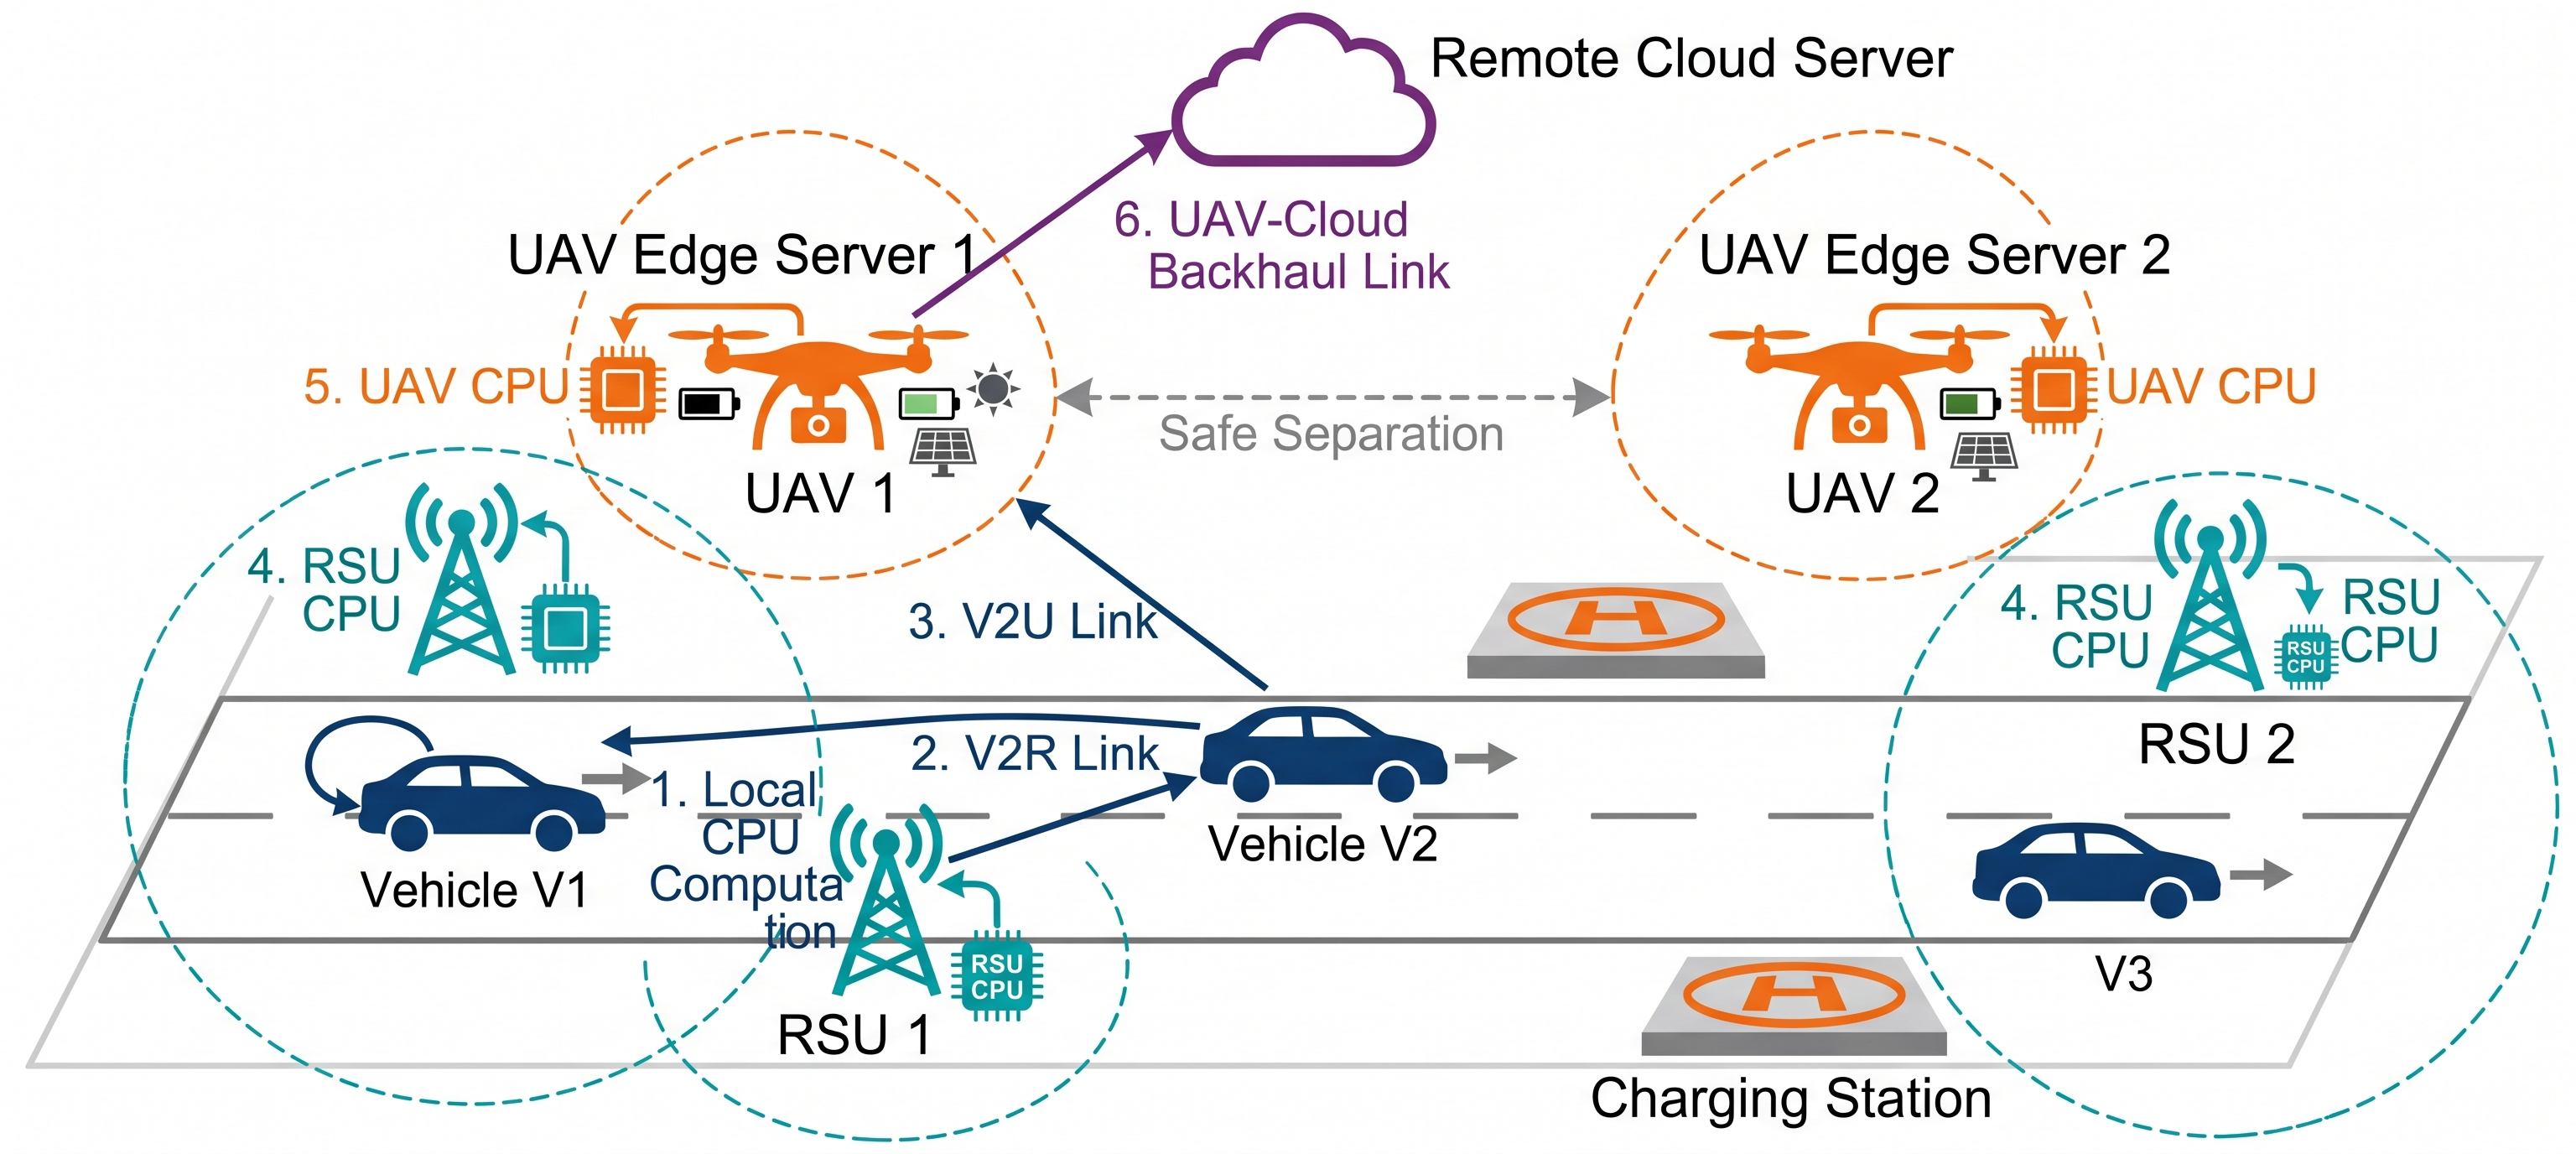
\includegraphics[width=0.94\textwidth]{Network architecture diagram.png}
\par\vspace{2pt}
{\footnotesize (a) Vehicle--RSU--UAV--cloud architecture.\par}
\vspace{5pt}
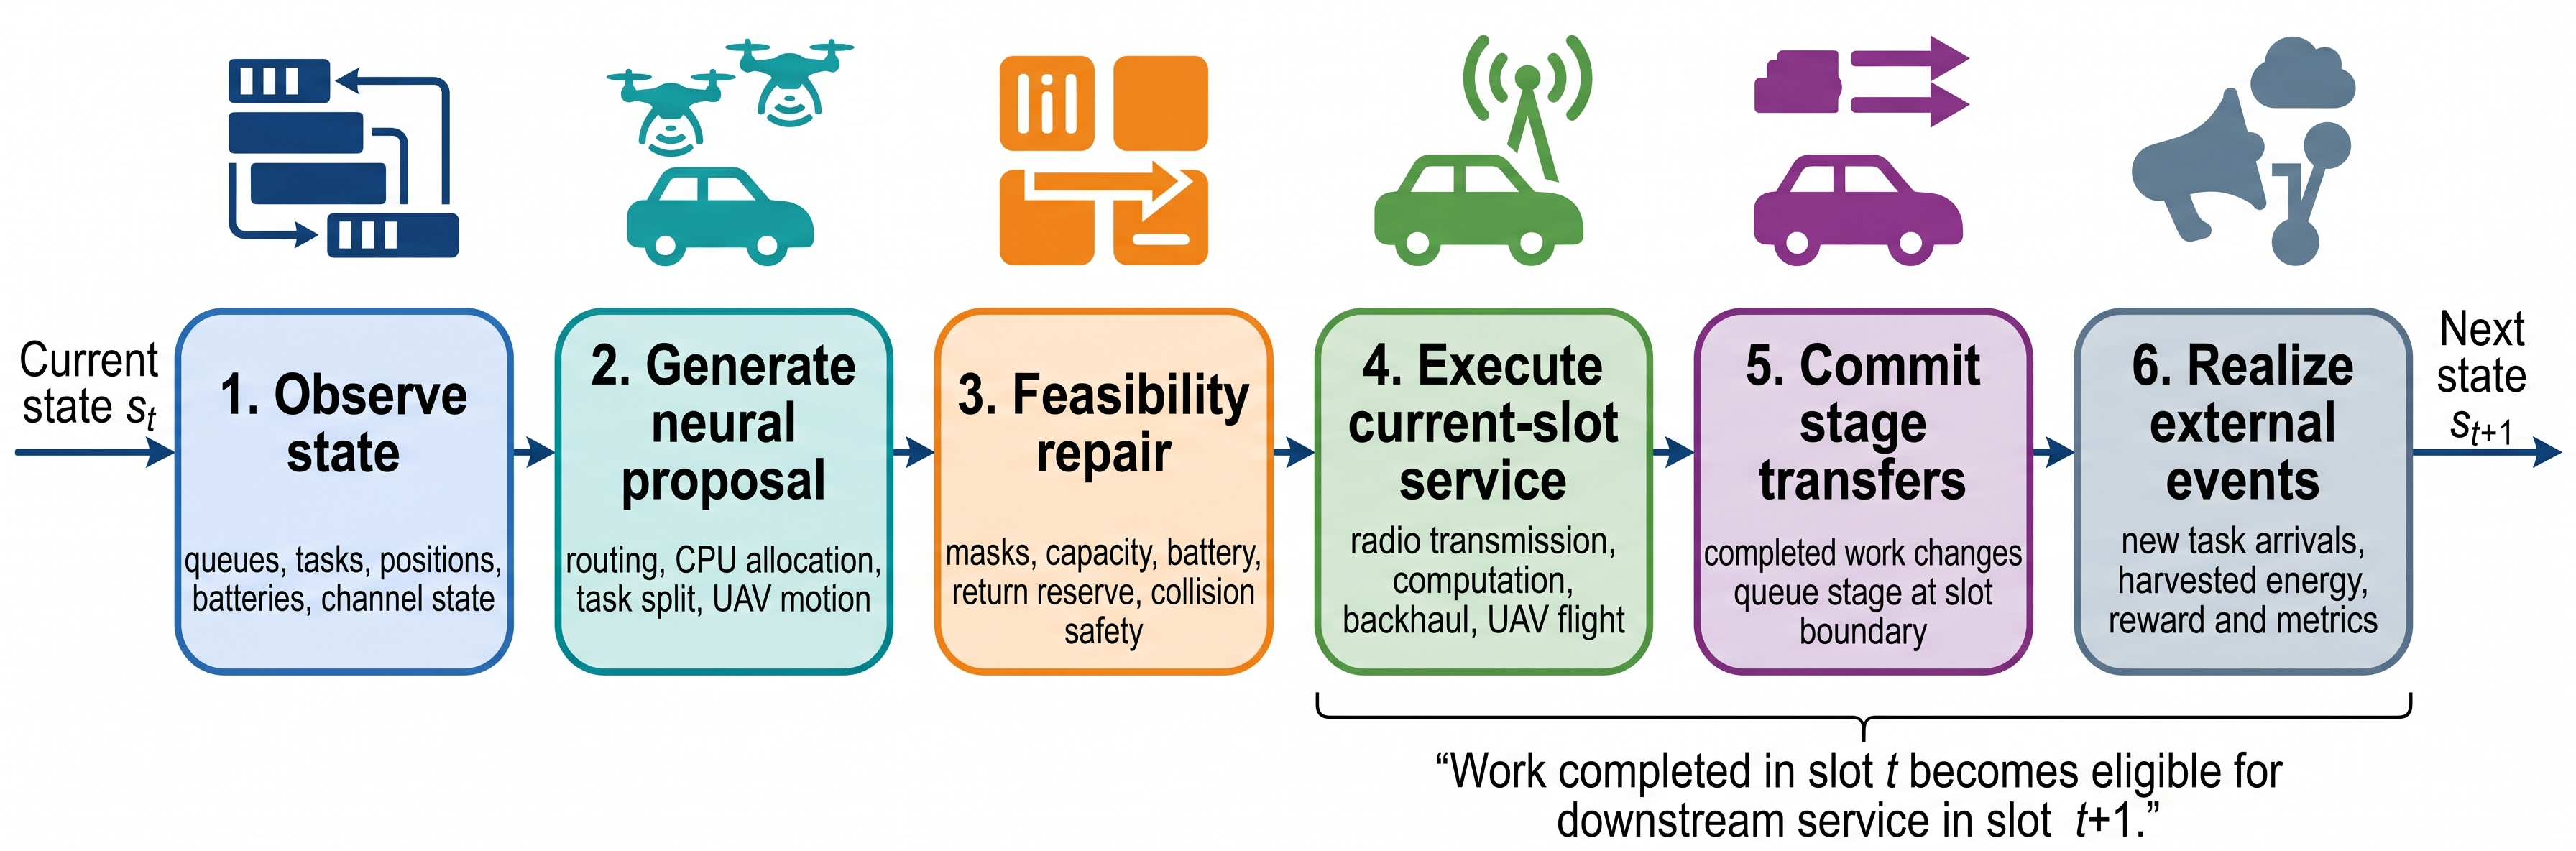
\includegraphics[width=0.96\textwidth]{Causal time-slot execution workflow.png}
\par\vspace{2pt}
{\footnotesize (b) Causal execution order within slot $t$.\par}
\caption{System architecture and causal slot execution. RSUs supply fixed
edge capacity and UAVs supply mobile edge service; work sent to a UAV may
keep a finite cloud branch. Harvested energy and external arrivals are
committed only after the service and expenditure of the current slot.}
\label{fig:network_slot}
\end{figure*}

\begin{figure*}[t]
\centering
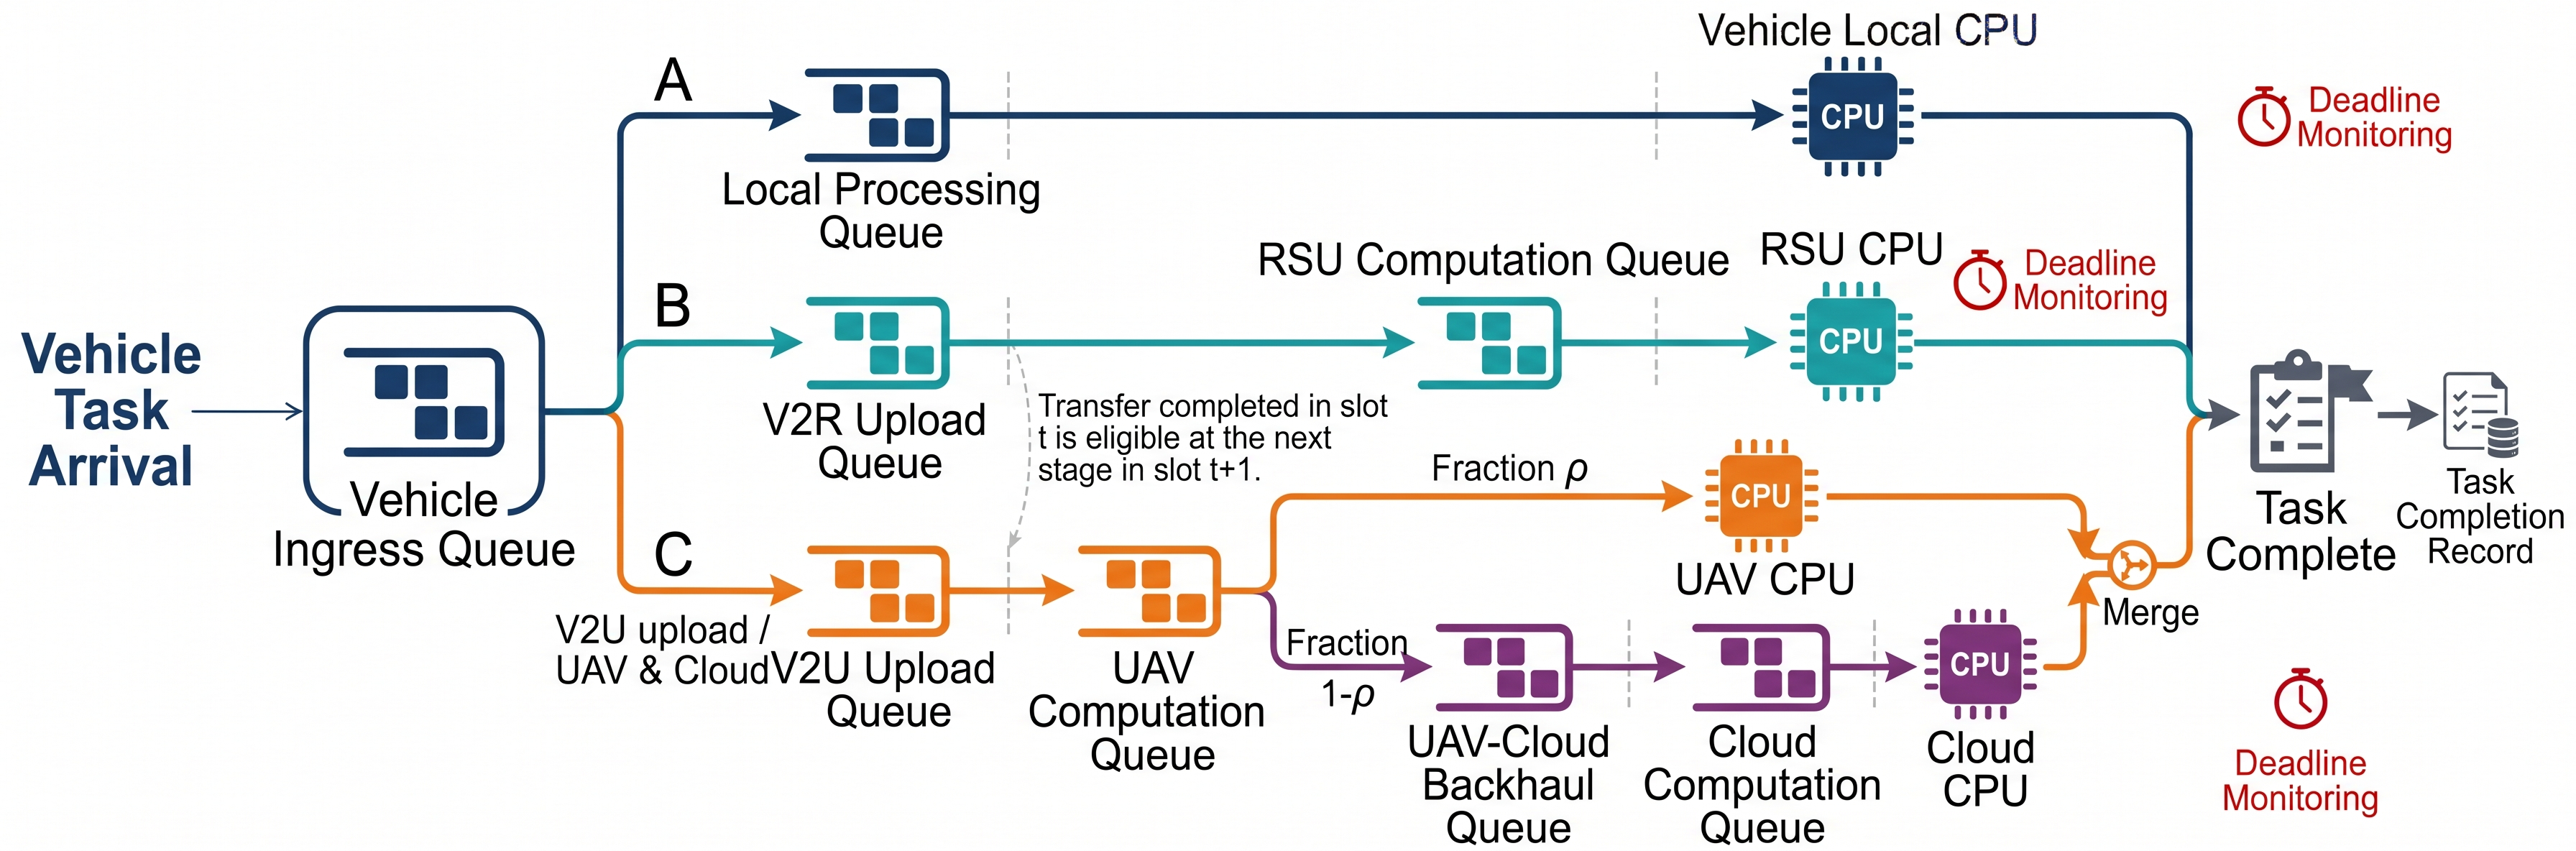
\includegraphics[width=0.96\textwidth]{End-to-end task lifecycle and queue mode.png}
\caption{End-to-end task service graph. Each box corresponds to a persistent
task or queue stage. A transfer committed at one boundary becomes eligible at
the next one.}
\label{fig:service_graph}
\end{figure*}

The core architecture leaves out a few options on purpose. There is no
direct vehicle-to-cloud or RSU-to-cloud route, tasks are not migrated between
UAVs, and nothing is reassigned after dispatch. Transmit powers are fixed and
the uplinks use orthogonal bandwidth. These restrictions let us study the
routing, CPU, split and trajectory decisions in isolation.

\begin{table*}[t]
\centering
\caption{Principal system notation.}
\label{tab:notation}
\renewcommand{\arraystretch}{1.12}
\begin{tabular}{p{0.13\textwidth}p{0.31\textwidth}p{0.13\textwidth}p{0.30\textwidth}}
\hline
\textbf{Symbol} & \textbf{Meaning} & \textbf{Symbol} & \textbf{Meaning}\\
\hline
$\Delta$ & Slot duration &
$\ell_i$ & Immutable task specification\\
$b_i,c_i,\chi_i$ & Input bits, CPU cycles, cycles per bit &
$a_i,d_i$ & Arrival time and deadline allowance\\
$Q_j(t)$ & Equivalent-cycle backlog of stage queue $j$ &
$A_j(t),S_j(t)$ & Realized queue arrival and service\\
$W_{ih}(t),R_{ih}(t)$ & Link bandwidth and transmission rate &
$f_n(t),w_{in}(t)$ & CPU frequency and task share\\
$B_k(t),H_k(t)$ & Physical UAV charge and harvested energy &
$Z_k(t)$ & Virtual net-energy deficit\\
$\boldsymbol p_v,\boldsymbol p_r,\boldsymbol p_k$ &
Vehicle, RSU, and UAV positions &
$\rho_i$ & UAV-local workload fraction\\
\hline
\end{tabular}
\end{table*}

\subsection{Vehicle Mobility and Coverage Model}
Synthetic vehicles drive along declared road polylines. The map
$\boldsymbol r_v(s)$ takes a route distance $s\in[0,L_v]$ to a 3-D road
coordinate, and $\nu_v(t)\ge0$ is the speed of the vehicle. Progress along the
route evolves as
\begin{equation}
\begin{aligned}
s_v(t+1)&=\mathscr R_v\!\left(
s_v(t)+\sigma_v(t)\nu_v(t)\Delta\right),\\
\boldsymbol p_v(t)&=\boldsymbol r_v(s_v(t)),
\end{aligned}
\label{eq:vehicle_motion}
\end{equation}
where $\sigma_v(t)\in\{-1,1\}$ gives the direction of travel and
$\mathscr R_v$ either wraps progress around a loop or reflects it at the end
of a route. In experiments with recorded SUMO traces,
Eq.~\eqref{eq:vehicle_motion} is replaced by the full sampled trace
$\boldsymbol p_v(t)=\boldsymbol p_v^{\mathrm{trace}}(t)$. Traces with missing
vehicle frames are rejected; we do not interpolate them.

For vehicle $v$ and edge node $n\in\mathcal R\cup\mathcal U$, the
three-dimensional distance and its horizontal component are
\begin{equation}
d_{vn}(t)=\|\boldsymbol p_v(t)-\boldsymbol p_n(t)\|,\qquad
d_{vn}^{\mathrm H}(t)=
\|[\boldsymbol p_v(t)-\boldsymbol p_n(t)]_{1:2}\|.
\label{eq:distances}
\end{equation}
Coverage is indicated by
$\mathbf 1\{d_{vr}^{\mathrm H}\le D_R\}$ for an RSU and by
$\mathbf 1\{d_{vk}^{\mathrm H}\le D_U\}$ for a UAV. We mask a destination if
it is out of coverage or inactive, if it is a UAV on its way back, or if no
admissible energy contingency exists for it.

\subsection{Task Generation, Lifecycle, and Offloading Model}
\label{subsec:task_model}
\subsubsection{Task Arrival and Persistent Record Model}
In slot $t$, vehicle $v$ produces $A_v^{\mathrm{task}}(t)$ jobs. For the
controlled synthetic benchmark we use
\begin{equation}
\begin{aligned}
A_v^{\mathrm{task}}(t)&\sim
\operatorname{Poisson}(\lambda_v(t)),\\
b_i&\in[b_{\min},b_{\max}],\quad
c_i\in[c_{\min},c_{\max}],\\
d_i&\in[d_{\min},d_{\max}],
\end{aligned}
\label{eq:task_arrival}
\end{equation}
where the draws are bounded and independent and are stored once in a
scenario trace. The low-load, near-capacity, overload, and surge cases are
distinguished through $\lambda_v(t)$. Every task carries the immutable record
\begin{equation}
\ell_i=(i,v(i),b_i,c_i,a_i,d_i,\zeta_i),\qquad
\chi_i=\frac{c_i}{b_i},
\label{eq:task_record}
\end{equation}
in which $\zeta_i\in\{0,1\}$ states whether the job can be partitioned.

\subsubsection{Destination Selection and Partitioning Model}
The indicator $h_i(t)$ means that the task is held in ingress, and $x_i^L(t)$,
$x_{ir}^R(t)$, and $x_{ik}^U(t)$ indicate dispatch to local execution, to an
RSU, and to a UAV. Before dispatch,
\begin{equation}
h_i(t)+x_i^L(t)+\sum_{r\in\mathcal R}x_{ir}^R(t)
 +\sum_{k\in\mathcal U}x_{ik}^U(t)=1,
\quad x,h\in\{0,1\}.
\label{eq:destination}
\end{equation}
With $h_i=1$ the task stays in ingress. As soon as any other choice is made,
the destination and the dispatch time can no longer change.

When a UAV is chosen, the whole input is uploaded to it first. The UAV then
executes a fraction $\rho_i$ of the work and forwards the rest to the cloud:
\begin{equation}
c_i^U=\rho_i c_i,\qquad
c_i^c=(1-\rho_i)c_i,\qquad
b_i^{\mathrm{bh}}=(1-\rho_i)b_i.
\label{eq:split}
\end{equation}
Indivisible work has $\rho_i=1$. For partitionable work, a value
$0\le\rho_i\le1$ is chosen at dispatch and then kept. A task is complete only
when every nonempty branch has finished and the merge delay
$\tau_i^{\mathrm{merge}}$ has passed.

\subsubsection{End-to-End Completion and Delay Model}
Given the actual completion time $f_i^{\mathrm{done}}$, the response time and
the deadline-success indicator are
\begin{equation}
T_i=f_i^{\mathrm{done}}-a_i,\qquad
\delta_i=\mathbf 1\{T_i\le d_i\}.
\label{eq:actual_latency}
\end{equation}
A miss is logged at the moment a task first crosses its deadline, and the
simulator keeps tracking the work that remains. A task that is still
unfinished when the trace ends is reported as censored, and we do not impute
a completion latency for it.

\subsection{Communication and OFDMA Service Model}
\subsubsection{Vehicle-to-RSU Terrestrial Channel Model}
On a vehicle--RSU link, the large-scale gain is deterministic:
\begin{equation}
g_{vr}^{R}(t)=g_0
\max\{d_{vr}(t),d_{\min}^{\mathrm{ch}}\}^{-\alpha_R},
\label{eq:rsu_gain}
\end{equation}
with reference gain $g_0$ and terrestrial path-loss exponent $\alpha_R$.

\subsubsection{Vehicle-to-UAV Air-to-Ground Channel Model}
On a vehicle--UAV link, the elevation angle and the LoS probability are
\begin{equation}
\begin{aligned}
\vartheta_{vk}(t)&=
\frac{180}{\pi}\tan^{-1}\!\left(
\frac{|z_k(t)-z_v(t)|}
{\max\{d_{vk}^{\mathrm H}(t),d_{\min}^{\mathrm{ch}}\}}\right),\\
p_{vk}^{\mathrm{LoS}}(t)&=
\left[1+a_{\mathrm L}
\exp\{-b_{\mathrm L}[\vartheta_{vk}(t)-a_{\mathrm L}]\}\right]^{-1}.
\end{aligned}
\label{eq:los}
\end{equation}
The mean aerial gain is then
\begin{equation}
\begin{aligned}
g_{vk}^{U}(t)={}&g_0
\max\{d_{vk}(t),d_{\min}^{\mathrm{ch}}\}^{-\alpha_U}\\
&\times\left[p_{vk}^{\mathrm{LoS}}\eta_{\mathrm L}
+(1-p_{vk}^{\mathrm{LoS}})\eta_{\mathrm N}\right],
\end{aligned}
\label{eq:uav_gain}
\end{equation}
in which the factors $\eta_{\mathrm L}=10^{-L_{\mathrm L}/10}$ and
$\eta_{\mathrm N}=10^{-L_{\mathrm N}/10}$ model the extra losses under LoS
and NLoS conditions.

\subsubsection{OFDMA Rate and Transmission-Service Model}
Suppose link $h$ is given bandwidth $W_{ih}(t)$ and has gain $g_{ih}(t)$,
and the vehicle transmits at fixed power $P_v^{\mathrm{tx}}$. Its rate is
then
\begin{equation}
R_{ih}(t)=W_{ih}(t)\log_2\!\left(
1+\frac{P_v^{\mathrm{tx}}g_{ih}(t)}
{N_0W_{ih}(t)+I_{ih}(t)}\right).
\label{eq:rate}
\end{equation}
Because the links are orthogonal, $I_{ih}=0$ and
$\sum_iW_{ih}\le W_h^{\max}$.

All controllers use the same deterministic scheduler, which assigns the
priority
\begin{equation}
\begin{aligned}
\pi_{ih}(t)&=q_{ih}^{\mathrm{eq}}(t)
\left[1+\min\left\{\frac{\operatorname{age}_i(t)}{d_i},
\kappa_{\mathrm{age}}\right\}\right],\\
W_{ih}(t)&=W_h^{\max}
\frac{\pi_{ih}(t)}{\sum_{\ell\in\mathcal E_h}\pi_{\ell h}(t)}.
\end{aligned}
\label{eq:ofdma}
\end{equation}
over the eligible links $\mathcal E_h$; exact ties are broken by task ID.
The term $q_{ih}^{\mathrm{eq}}$ is the backlog of the link expressed in
equivalent cycles. Any transfer of $s_{ih}^{\mathrm{tr}}$ equivalent cycles
has to satisfy
\begin{equation}
\sum_i\frac{s_{ih}^{\mathrm{tr}}(t)}{\chi_i}
\le\Delta R_h(t).
\label{eq:radio_capacity}
\end{equation}
A link that loses coverage serves nothing in that slot, and the bits it has
not yet sent stay in the upload queue where they started.

\subsection{Computation, Backhaul, and Queueing Model}
\subsubsection{Persistent Multi-Stage Queue Model}
The set $\mathcal J$ holds one queue per stage: ingress, V2R/V2U upload,
receive/staging, local/RSU/UAV compute, UAV backhaul, cloud receive, and
cloud compute. Queues measured in bits are converted to cycles only for the
drift accounting, with $b$ residual bits of task $i$ counted as $\chi_i b$
cycles.

Given the realized service $S_j(t)$ and arrivals $A_j(t)$, each queue $j$
evolves as
\begin{equation}
Q_j(t+1)=Q_j(t)-S_j(t)+A_j(t),\qquad
0\le S_j(t)\le Q_j(t).
\label{eq:queue}
\end{equation}
When a flow $F_{ab}(t)$ of equivalent work goes from stage $a$ to stage $b$,
it enters the increment of the source with a minus sign, $-F_{ab}$, and the
increment of the destination as $+F_{ab}$. Summing over all queues gives
\begin{equation}
\sum_{j\in\mathcal J}Q_j(t+1)=
\sum_{j\in\mathcal J}Q_j(t)+A^{\mathrm{ext}}(t)-C^{\mathrm{final}}(t),
\label{eq:conservation}
\end{equation}
apart from the branch creation and merge bookkeeping, which is logged
explicitly. Work is never lost through internal routing; it leaves the
system only when its final computation is done.

\subsubsection{CPU Service and Processor-Sharing Model}
For compute node $n$, the frequency $f_n$, the task shares $w_{in}$, and the
residual work that is ready, $c_{in}^{\mathrm{elig}}$, must satisfy
\begin{equation}
\begin{aligned}
0&\le f_n(t)\le f_n^{\max},\\
w_{in}(t)&\ge0,\qquad \sum_iw_{in}(t)\le1,\\
0\le s_{in}^{\mathrm{cpu}}(t)&\le
\min\{c_{in}^{\mathrm{elig}}(t),\Delta f_n(t)w_{in}(t)\}.
\end{aligned}
\label{eq:cpu_capacity}
\end{equation}
If a task finishes early, the capacity it leaves unused is shared out among
the other tasks that still have a positive share. In the core experiments,
scheduling on the vehicles and in the cloud is fixed, and so is the RSU clock
frequency. The controller sets the RSU task shares and, for each UAV, both the
frequency and the task shares.

\subsubsection{UAV Backhaul and Cloud-Service Model}
Before reaching the cloud, the cloud branch of a UAV task $i$ has to cross a
finite backhaul:
\begin{equation}
\sum_{i\in\mathcal B_k(t)}
\frac{s_{ik}^{\mathrm{bh}}(t)}{\chi_i}
\le\Delta R_k^{\mathrm{bh}},
\qquad
\sum_i s_{ic}^{\mathrm{cpu}}(t)\le\Delta f_c.
\label{eq:cloud_capacity}
\end{equation}
Once the backhaul transfer is done, $(1-\rho_i)c_i$ cycles are released to
cloud computation at the following boundary. The task is finished only when
both the UAV branch and the cloud branch (where nonempty) are complete.

\subsubsection{Queue-Stability Target}
We aim for the strong-stability condition
\begin{equation}
\limsup_{T\to\infty}\frac1T\sum_{t=0}^{T-1}
\mathbb E[Q_j(t)]<\infty,\qquad j\in\mathcal J.
\label{eq:stability}
\end{equation}
It only makes sense when the offered load can be stabilized, and in the
overload experiments we deliberately report the queue growth instead.

\subsection{UAV Movement and Collision-Avoidance Model}
With horizontal speed $v_k^{\mathrm H}$, azimuth $\theta_k$, and vertical
speed $v_k^z$, the velocity and the position are updated as
\begin{equation}
\begin{aligned}
\boldsymbol u_k(t)&=
\begin{bmatrix}
v_k^{\mathrm H}\cos\theta_k&
v_k^{\mathrm H}\sin\theta_k&v_k^z
\end{bmatrix}^{\mathsf T},\\
\boldsymbol p_k(t+1)&=\boldsymbol p_k(t)+\Delta\boldsymbol u_k(t).
\end{aligned}
\label{eq:uav_motion}
\end{equation}
A motion is admissible only if it stays within the speed, climb/descent,
map, altitude, and acceleration bounds:
\begin{equation}
\begin{aligned}
\|\boldsymbol u_k(t)\|&\le v_k^{\max},\\
-v_k^{\mathrm{down}}&\le v_k^z(t)\le v_k^{\mathrm{up}},\\
\|\boldsymbol u_k(t)-\boldsymbol u_k(t-1)\|&\le a_k^{\max}\Delta.
\end{aligned}
\label{eq:flight_bounds}
\end{equation}
Any two airborne UAVs must also keep their distance along the entire linear
trajectory of the slot:
\begin{equation}
\min_{\tau\in[0,\Delta]}
\|\boldsymbol p_k(t)+\tau\boldsymbol u_k(t)
-\boldsymbol p_l(t)-\tau\boldsymbol u_l(t)\|
\ge d_{\mathrm{safe}}.
\label{eq:collision}
\end{equation}
In addition, the controller keeps enough stopping distance from the map and
altitude boundaries. We call a return/landing plan verified when it consists
of segments that respect the same limits and ends at a declared landing site
with almost zero velocity.

\subsection{UAV and Infrastructure Energy-Consumption Models}
Fig.~\ref{fig:energy_safety_overview} gives an overview of the UAV energy
ledger, the replenishment paths, the flight constraints and the
return-reserve rule. Its laser-transfer branch is optional and was not active
in the stochastic-harvesting benchmark we report.

\begin{figure*}[!t]
\centering
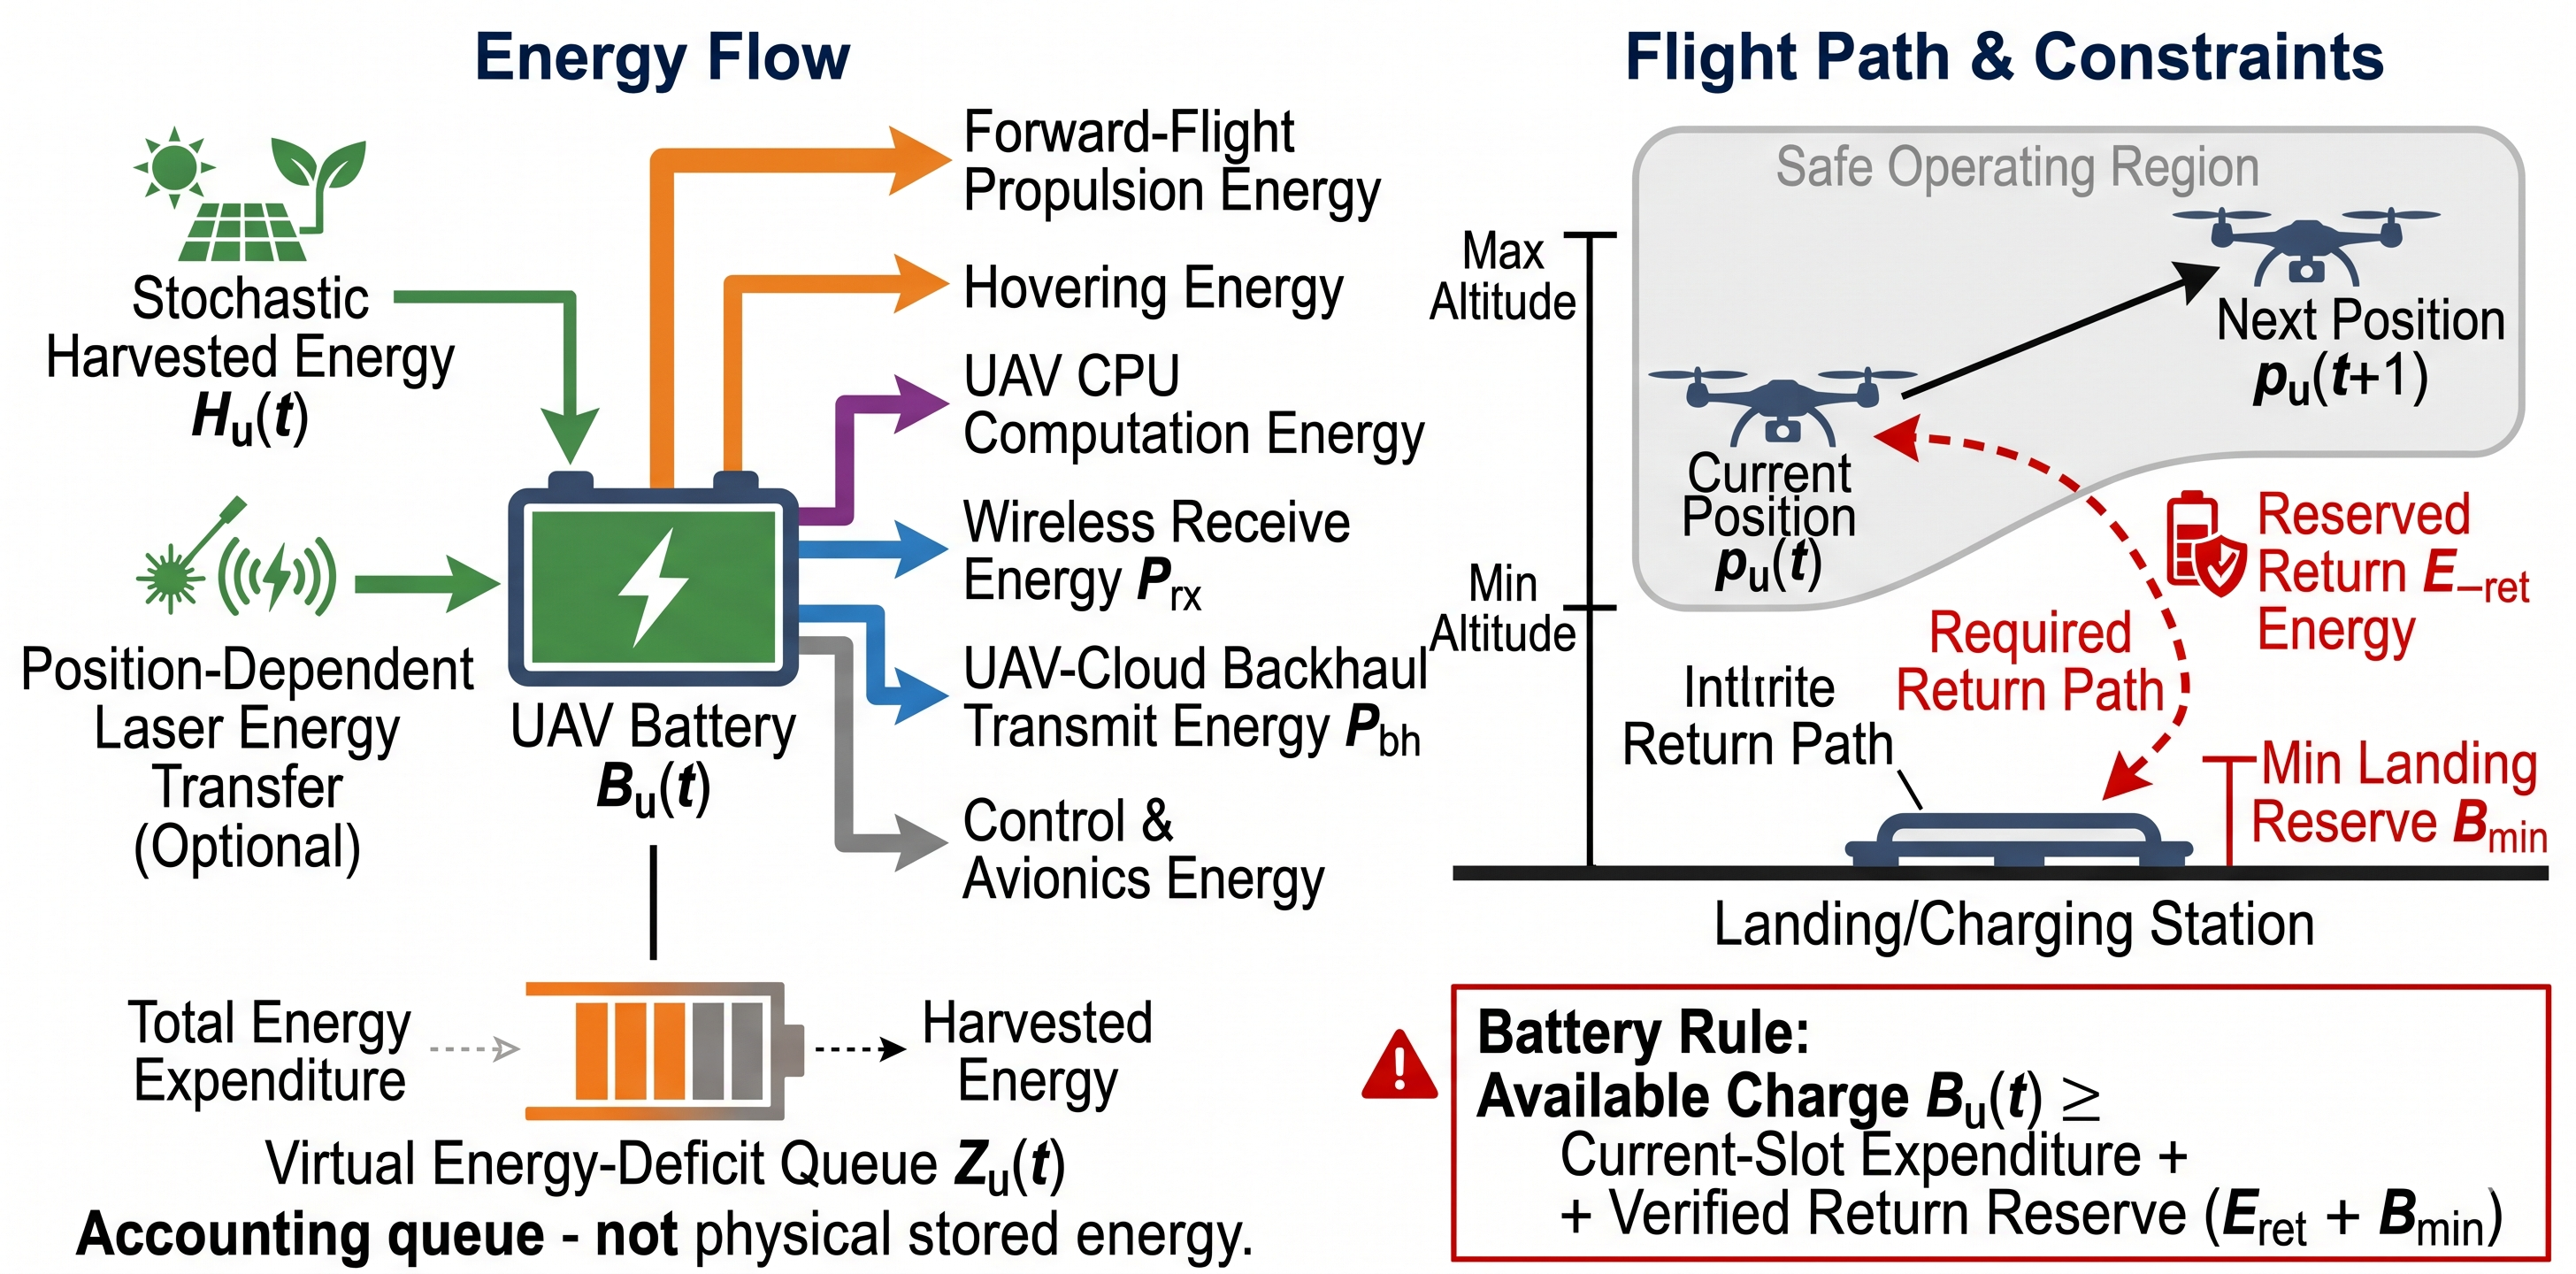
\includegraphics[width=0.94\textwidth]{UAV energy, harvesting, and return-reserve model.png}
\caption{UAV energy, harvesting, and return-reserve model. The physical
battery pays for propulsion, computation, communication, and control. Normal
service is allowed only while the current expenditure and a verified return
or landing reserve can both be met. The virtual deficit is a bookkeeping
queue; it does not store energy.}
\label{fig:energy_safety_overview}
\end{figure*}

\subsubsection{Rotary-Wing Flight and Hovering-Energy Model}
As in the energy accounting of~\cite{talukdar2026mappo}, the propulsion
ledger keeps motion and hovering apart. In slot $t$, let
$\tau_k^{\mathrm{fly}}(t)$ be the time spent in airborne flight and
$\tau_k^{\mathrm{hov}}(t)$ the time spent hovering at near-zero velocity,
where $\tau_k^{\mathrm{fly}}+\tau_k^{\mathrm{hov}}\le\Delta$. While flying,
the horizontal and vertical power is modeled as
\begin{equation}
\begin{aligned}
P_k^{\mathrm{fly}}={}&P_0\!\left(1+
\frac{c_p(v_k^{\mathrm H})^2}{U_{\mathrm{tip}}^2}\right)\\
&+P_i\!\left(\sqrt{1+\frac{(v_k^{\mathrm H})^4}{4v_0^4}}\right.\\
&\left.\hspace{3.1em}-\frac{(v_k^{\mathrm H})^2}{2v_0^2}\right)^{1/2}\\
&+c_d(v_k^{\mathrm H})^3
+c_{\uparrow}[v_k^z]^+
+c_{\downarrow}[-v_k^z]^+
+c_z(v_k^z)^2 .
\end{aligned}
\label{eq:propulsion}
\end{equation}
In this expression, $P_0$ is the blade-profile hover power and $P_i$ the
induced hover power, $U_{\mathrm{tip}}$ is the rotor-tip speed, and $v_0$ is
the mean induced velocity in hover. The other coefficients are calibrated and
capture horizontal drag as well as ascent and descent. When both the
horizontal and the vertical velocity are close to zero, the model reduces to
the hovering power
\begin{equation}
\begin{aligned}
P_k^{\mathrm{hov}}&=P_0+P_i,\\
E_k^{\mathrm{fly}}(t)&=P_k^{\mathrm{fly}}(t)
 \tau_k^{\mathrm{fly}}(t),\\
E_k^{\mathrm{hov}}(t)&=P_k^{\mathrm{hov}}
 \tau_k^{\mathrm{hov}}(t),\\
E_k^{\mathrm{prop}}(t)&=E_k^{\mathrm{fly}}(t)
 +E_k^{\mathrm{hov}}(t).
\end{aligned}
\label{eq:hovering}
\end{equation}
With this split, hover time is never billed a second time as flight. The present
implementation is piecewise constant over a slot: a nonzero airborne motion
command gives $(\tau_k^{\mathrm{fly}},\tau_k^{\mathrm{hov}})=(\Delta,0)$, and
an airborne hover gives $(0,\Delta)$. Writing the two intervals separately
leaves room for sub-slot scheduling later on. Any remaining part of the slot
belongs to a landed or otherwise non-airborne mode, for which the airborne
propulsion power is zero. We note that Eq.~\eqref{eq:propulsion} is a
calibrated approximation for bounded flight and not a complete aerodynamic
model.

\subsubsection{Computation and Communication-Energy Model}
UAV $k$ computes $s_k^{\mathrm{cpu}}$ cycles. While it receives uplink data
from vehicles, its receiver chain draws power $P_k^{\mathrm{rx}}$ over an
active reception time $\tau_k^{\mathrm{rx}}$. In the same way, the UAV
transmits on the UAV--cloud backhaul with power $P_k^{\mathrm{bh}}$ for an
active time $\tau_k^{\mathrm{bh}}$. The avionics and control electronics,
which run whenever the UAV is active, are covered by $P_k^{\mathrm{ctrl}}$
and $\tau_k^{\mathrm{ctrl}}$. All powers are in watts and all active times in
seconds, so each product is an energy in joules. The individual energy terms
are
\begin{equation}
\begin{aligned}
E_k^{\mathrm{cpu}}&=\kappa_k f_k^2s_k^{\mathrm{cpu}},\\
E_k^{\mathrm{rx}}&=P_k^{\mathrm{rx}}\tau_k^{\mathrm{rx}},&
E_k^{\mathrm{bh}}&=P_k^{\mathrm{bh}}\tau_k^{\mathrm{bh}},\\
E_k^{\mathrm{ctrl}}&=P_k^{\mathrm{ctrl}}\tau_k^{\mathrm{ctrl}}.&&
\end{aligned}
\label{eq:energy_components}
\end{equation}
Adding these terms, the total UAV expenditure is
\begin{equation}
E_k=E_k^{\mathrm{fly}}+E_k^{\mathrm{hov}}+E_k^{\mathrm{cpu}}
+E_k^{\mathrm{rx}}+E_k^{\mathrm{bh}}+E_k^{\mathrm{ctrl}}.
\label{eq:uav_energy}
\end{equation}
A vehicle spends $P_v^{\mathrm{tx}}\tau_v^{\mathrm{tx}}$ on its uplink. The
compute energy of RSUs and of the cloud follows the same
$\kappa_nf_n^2s_n^{\mathrm{cpu}}$ rule, and their receiver energy is charged
separately. In the system energy, each ownership component is counted once.

\subsection{Energy-Harvesting, Battery, and Return-Reserve Model}
\subsubsection{Stochastic Energy-Replenishment Model}
In the implementation, energy is replenished according to the trace
\begin{equation}
H_k(t)=I_k^{\mathrm{src}}(t)\,\bar H_k\,\xi_k(t),\qquad
\xi_k(t)\sim\mathcal U[1-\delta_H,1+\delta_H],
\label{eq:stochastic_harvest}
\end{equation}
with $I_k^{\mathrm{src}}(t)=0$ during a declared outage and
$I_k^{\mathrm{src}}(t)=1$ at all other times. We use $\delta_H=0.2$ in the benchmark and set
$\bar H_k=0$ in the zero-harvest scenarios. Each realization is drawn once,
and all compared controllers see the same one.

\subsubsection{Optional Position-Dependent Laser-Transfer Model}
Should a laser source located at $\boldsymbol p_L$ be added later, the
following optional model makes the harvested energy depend on position:
\begin{equation}
\begin{aligned}
d_{Lk}(t)&=\|\boldsymbol p_k(t)-\boldsymbol p_L\|,\\
P_k^{\mathrm{rec}}(t)&=
P_L(t)\frac{A_k}{[\theta_Ld_{Lk}(t)]^2}
\exp[-\kappa_{\mathrm{atm}}(t)d_{Lk}(t)]
\eta_k^{\mathrm{align}}(t),\\
H_k^{\mathrm{laser}}(t)&=\Delta\eta_k^{\mathrm{pv}}
P_k^{\mathrm{rec}}(t).
\end{aligned}
\label{eq:optional_laser}
\end{equation}
Using it would require calibrated values for the beam divergence, atmospheric
attenuation, alignment, aperture, and photovoltaic efficiency. The current
stochastic benchmark does not include it.

\subsubsection{Battery Evolution, Energy Causality, and Landing Reserve}
We write $B_k^{\mathrm{pre}}(t+1)$ for the charge left right after the
slot's expenditure and before the end-of-slot replenishment. The battery then
obeys
\begin{equation}
\begin{aligned}
B_k^{\mathrm{pre}}(t+1)&=B_k(t)-E_k(t),\\
B_k(t+1)&=\min\{B_k^{\max},
B_k^{\mathrm{pre}}(t+1)+H_k(t)\},\\
0&\le B_k(t)\le B_k^{\max},\qquad
0\le E_k(t)\le B_k(t).
\end{aligned}
\label{eq:battery}
\end{equation}
This ordering means that harvested energy becomes usable only after the
current expenditure has been paid; it cannot fund an action taken earlier in
the same slot. To
combine a declared emergency floor with a return-safety margin that depends
on the state, we define
$B_k^{\min}=\xi_kB_k^{\max}$ for $\xi_k\in[0,1)$ when such a floor is
specified (and $B_k^{\min}=0$ otherwise), and
\[
B_k^{\mathrm{safe}}(t+1)=\max\!\left\{B_k^{\min},
B_k^{\mathrm{res}}(\boldsymbol p_k(t+1),\boldsymbol u_k(t))\right\}.
\]
During normal service, the following stronger energy-causality constraint
must hold:
\begin{equation}
B_k^{\mathrm{pre}}(t+1)\ge B_k^{\mathrm{safe}}(t+1).
\label{eq:reserve}
\end{equation}
The quantity $B_k^{\mathrm{res}}$ is the energy needed for a verified
return/landing plan, computed without counting on any future harvest. Battery
overflow, $O_k(t)=[B_k^{\mathrm{pre}}(t+1)+H_k(t)-B_k^{\max}]^+$, is logged
but not credited as usable energy. If a UAV cannot keep
Eq.~\eqref{eq:reserve} satisfied, it switches to a verified return/landing
contingency, and UAVs that are returning or have landed cannot be chosen as
new destinations.

\section{Problem Formulation}
\label{problem_formulation}

The component models are linked through four kinds of controller decision:
dispatch, partitioning, CPU allocation and UAV motion. This section first
defines the per-slot cost used by the learning and Lyapunov layers and then
states the long-term stochastic optimization problem, with every physical
constraint written out.

\subsection{Instantaneous Cost Model}
Let $N(t)$ be the number of unfinished tasks and $M(t)$ the number of tasks
that cross their deadline for the first time in slot $t$. We use the
normalized instantaneous cost
\begin{equation}
C(t)=w_L\frac{\Delta N(t)}{L_{\mathrm{ref}}}
+w_E\frac{E^{\mathrm{sys}}(t)}{E_{\mathrm{ref}}}
+w_DM(t).
\label{eq:cost}
\end{equation}
The references are fixed so that costs can be compared between scenarios.
For a drained trace, the summed occupancy approximates the aggregate sojourn
time; the latency we report, however, is always computed from
Eq.~\eqref{eq:actual_latency}.

\subsection{Long-Term Stochastic Optimization Problem}
The vector $\boldsymbol\alpha(t)$ gathers every dispatch, split, CPU, and
motion decision. To keep the notation short, we write
$\mathcal D_i=\{L(i)\}\cup\mathcal R\cup\mathcal U$ for the candidate
destinations of task $i$ and use $m_{in}(t)\in\{0,1\}$ to show whether
destination $n$ is open to this task in slot $t$. The mask is set to zero for
a link without coverage, for a UAV that is returning or has landed, and for
any destination that fails the physical safety checks. The long-run problem
reads
\begin{equation}
\begin{aligned}
\mathcal P:\quad \min_{\pi}\;&
\limsup_{T\to\infty}\frac1T
\sum_{t=0}^{T-1}\mathbb E_{\pi}[C(t)].
\end{aligned}
\label{eq:problem}
\end{equation}
Instead of folding feasibility into a single set symbol, we list the
constraints one by one below. Unless another quantifier is given, each must
hold in every slot and for every task, applicable node, and UAV.

\stepcounter{equation}
\begin{equation}
\begin{gathered}
h_i(t)+\sum_{n\in\mathcal D_i}x_{in}(t)=1,\\
h_i(t),x_{in}(t)\in\{0,1\}
\end{gathered}
\tag{C1}\label{con:routing}
\end{equation}
\stepcounter{equation}
\begin{equation}
x_{in}(t)\le m_{in}(t),\qquad n\in\mathcal D_i
\tag{C2}\label{con:mask}
\end{equation}
\stepcounter{equation}
\begin{equation}
0\le\rho_i(t)\le1,\qquad
\rho_i(t)=1\ \text{if }\zeta_i=0
\tag{C3}\label{con:split}
\end{equation}
By (C1), a task is either held, executed locally, offloaded to an RSU, or
offloaded to a UAV, and exactly one of these applies. (C2) rules out dispatch
over a link that is unavailable or to a UAV that is unsafe. (C3) allows a
cloud split only when the task is partitionable. After dispatch, the chosen
destination and split do not change.

\stepcounter{equation}
\begin{equation}
\begin{gathered}
s_{ih}^{\mathrm{tr}}(t)\ge0,\qquad
\sum_i\frac{s_{ih}^{\mathrm{tr}}(t)}{\chi_i}\le\Delta R_h(t),\\
W_{ih}(t)\ge0,\qquad \sum_iW_{ih}(t)\le W_h^{\max}
\end{gathered}
\tag{C4}\label{con:radio}
\end{equation}
\stepcounter{equation}
\begin{equation}
\begin{gathered}
0\le f_n(t)\le f_n^{\max},\qquad w_{in}(t)\ge0,\\
\sum_iw_{in}(t)\le1
\end{gathered}
\tag{C5}\label{con:processor}
\end{equation}
\stepcounter{equation}
\begin{equation}
0\le s_{in}^{\mathrm{cpu}}(t)\le
\min\{c_{in}^{\mathrm{elig}}(t),\Delta f_n(t)w_{in}(t)\}
\tag{C6}\label{con:cpu-service}
\end{equation}
\stepcounter{equation}
\begin{equation}
\begin{gathered}
\sum_{i\in\mathcal B_k(t)}\frac{s_{ik}^{\mathrm{bh}}(t)}{\chi_i}
\le\Delta R_k^{\mathrm{bh}},\\
\sum_i s_{ic}^{\mathrm{cpu}}(t)\le\Delta f_c
\end{gathered}
\tag{C7}\label{con:backhaul-cloud}
\end{equation}
\stepcounter{equation}
\begin{equation}
\begin{gathered}
0\le S_j(t)\le Q_j(t),\\
Q_j(t+1)=Q_j(t)-S_j(t)+A_j(t)
\end{gathered}
\tag{C8}\label{con:queue-causality}
\end{equation}
The limits on spectrum, processors, backhaul, the cloud, and queue service
are given by (C4)--(C8). In particular, a stage cannot serve more work than was
eligible when the slot began. Output from an upstream stage joins the
downstream queue only at the next slot boundary, so a task cannot pass
through several stages within one slot.

With $\mathcal A$ the horizontal operating region, the UAVs are subject to
\stepcounter{equation}
\begin{equation}
\begin{gathered}
\boldsymbol p_k(t+1)=\boldsymbol p_k(t)+\Delta\boldsymbol u_k(t),\\
\boldsymbol p_k^{\mathrm H}(t+1)\in\mathcal A,\qquad
z_k^{\min}\le z_k(t+1)\le z_k^{\max}
\end{gathered}
\tag{C9}\label{con:position}
\end{equation}
\stepcounter{equation}
\begin{equation}
\begin{gathered}
\|\boldsymbol u_k(t)\|\le v_k^{\max},\\
-v_k^{\mathrm{down}}\le u_k^z(t)\le v_k^{\mathrm{up}}
\end{gathered}
\tag{C10}\label{con:speed}
\end{equation}
\stepcounter{equation}
\begin{equation}
\|\boldsymbol u_k(t)-\boldsymbol u_k(t-1)\|
\le a_k^{\max}\Delta
\tag{C11}\label{con:acceleration}
\end{equation}
\stepcounter{equation}
\begin{equation}
\begin{aligned}
\min_{\tau\in[0,\Delta]}\|&\boldsymbol p_k(t)+\tau\boldsymbol u_k(t)\\
&-\boldsymbol p_l(t)-\tau\boldsymbol u_l(t)\|
\ge d_{\mathrm{safe}},\quad k\ne l
\end{aligned}
\tag{C12}\label{con:separation}
\end{equation}
Constraints (C9)--(C12) cover the kinematics, the flight region, altitude,
speed, climb and descent rates, acceleration, and separation along the
continuous path. The stopping distance a UAV needs to stay inside the region
is built into the feasibility mask of (C2); it is not something checked only
after the motion has been carried out.

\stepcounter{equation}
\begin{equation}
\begin{gathered}
B_k^{\mathrm{pre}}(t+1)=B_k(t)-E_k(t),\\
B_k(t+1)=\min\{B_k^{\max},B_k^{\mathrm{pre}}(t+1)+H_k(t)\},\\
0\le B_k(t+1)\le B_k^{\max}
\end{gathered}
\tag{C13}\label{con:battery-dynamics}
\end{equation}
\stepcounter{equation}
\begin{equation}
\begin{gathered}
0\le E_k(t)\le B_k(t),\\
B_k^{\mathrm{pre}}(t+1)\ge B_k^{\mathrm{safe}}(t+1)
\end{gathered}
\tag{C14}\label{con:energy-reserve}
\end{equation}
\stepcounter{equation}
\begin{equation}
\limsup_{T\to\infty}\frac1T\sum_{t=0}^{T-1}
\mathbb E_{\pi}[Q_j(t)]<\infty,\quad j\in\mathcal J
\tag{C15}\label{con:queue-stability}
\end{equation}
\stepcounter{equation}
\begin{equation}
\limsup_{T\to\infty}\frac1T\sum_{t=0}^{T-1}
\mathbb E_{\pi}[E_k(t)-H_k(t)]\le\bar e_k,\quad k\in\mathcal U
\tag{C16}\label{con:average-energy}
\end{equation}
\stepcounter{equation}
(C13) and (C14) encode the implemented timing, in which energy is spent
before the harvest arrives, together with the battery capacity (through the
clipped update), immediate energy causality, and the verified return/landing
reserve. (C15) is the strong-stability target for each physical queue; in the
tests that are overloaded on purpose, we measure whether it holds and do not
assume it. In (C16), choosing $\bar e_k=0$ asks for energy neutrality over
the long run, while $\bar e_k>0$ allows a declared average battery draw over
a finite mission. Deadlines enter the cost through $M(t)$. Imposing them as
hard constraints could make the problem infeasible, and a task that misses its
deadline simply stays in the physical queues until it is completed.


% The shorter first-draft model is retained temporarily as source history but
% disabled. The compiled report uses restored_system_model.tex above.
\iffalse
\section{System Model and Problem Formulation}
\subsection{Network and Time-Slot Model}
Consider vehicles $\mathcal V$, RSUs $\mathcal R$, MEC-enabled UAVs
$\mathcal U$, and one cloud server. Time is divided into slots
$t\in\{0,\ldots,T-1\}$ of duration $\Delta$. Vehicle $v$ has processor
frequency $f_v^{\max}$, RSU $r$ has $f_r^{\max}$, UAV $u$ has
$f_u^{\max}$, and the cloud has $f_c^{\max}$. UAV $u$ occupies
$\vect p_u(t)=[x_u(t),y_u(t),h_u(t)]^\mathsf T$ and vehicle $v$ occupies
$\vect w_v(t)=[x_v(t),y_v(t),0]^\mathsf T$.

The UAV kinematics are
\begin{align}
\vect p_u(t+1)&=\vect p_u(t)+\Delta\vect v_u(t),\\
\|\vect v_{u,xy}(t)\|_2&\le v_{xy}^{\max},\qquad
-v_d^{\max}\le v_{u,z}(t)\le v_c^{\max}.
\end{align}
Position, altitude, acceleration, and pairwise-separation constraints require
\begin{align}
\vect p_u(t)&\in\mathcal P,\\
\|\vect v_u(t)-\vect v_u(t-1)\|_2&\le a^{\max}\Delta,\\
\|\vect p_u(t)-\vect p_j(t)\|_2&\ge d^{\min},\quad u\ne j.
\end{align}

\subsection{Task Generation, Routing, and Deadlines}
A task $k$ arriving at vehicle $v_k$ is
\begin{equation}
\mathcal J_k=(a_k,D_k,C_k,L_k,\chi_k),
\end{equation}
where $a_k$ is its arrival slot, $D_k$ is input size in bits, $C_k$ is
required CPU cycles, $L_k$ is the deadline, and $\chi_k$ indicates whether
the workload is partitionable. The destination variable
\begin{equation}
z_k(t)\in\{\text{wait},\text{local},r\in\mathcal R,u\in\mathcal U\}
\end{equation}
selects waiting, local execution, or offloading. If a partitionable task is
uploaded to UAV $u$, fraction $\rho_{k,u}(t)\in[0,1]$ is assigned to the UAV
and the remainder is forwarded to the cloud. Non-partitionable work uses a
binary effective fraction.

Completion time is the first slot boundary at which all required upload,
computation, backhaul, and cloud stages finish. Task $k$ is on time if
\begin{equation}
t_k^{\mathrm{done}}\Delta-a_k\Delta\le L_k.
\end{equation}
Expired work is not silently discarded: it remains in the physical queues so
that overload and late completion remain observable.

\subsection{Wireless Communication Model}
For vehicle $v$ and UAV $u$, distance and elevation are
\begin{align}
d_{v,u}(t)&=\|\vect w_v(t)-\vect p_u(t)\|_2,\\
\theta_{v,u}(t)&=\frac{180}{\pi}\sin^{-1}
\left(\frac{h_u(t)}{d_{v,u}(t)}\right).
\end{align}
The line-of-sight probability is
\begin{equation}
P_{v,u}^{\mathrm{LoS}}(t)=
\frac{1}{1+a\exp[-b(\theta_{v,u}(t)-a)]},
\end{equation}
and the mean air-to-ground path loss combines LoS and NLoS excess losses.
Terrestrial vehicle--RSU links use a distance-dependent path-loss and fading
model. For link $\ell$ allocated bandwidth $W_\ell(t)$, power $P_\ell(t)$,
gain $g_\ell(t)$, noise density $N_0$, and interference $I_\ell(t)$,
\begin{equation}
R_\ell(t)=W_\ell(t)\log_2\left(1+
\frac{P_\ell(t)g_\ell(t)}{N_0W_\ell(t)+I_\ell(t)}\right).
\end{equation}
Each access node satisfies $\sum_{\ell\in\mathcal H_n}W_\ell(t)\le
W_n^{\max}$. Every learned controller uses the same deterministic radio
scheduler so that policy comparisons isolate control rather than spectrum
implementation.

\subsection{Persistent Multi-Stage Queue Model}
Let $Q_q(t)$ denote workload in queue $q$ at the beginning of slot $t$.
Queues represent vehicle upload, RSU/UAV computation, UAV backhaul, and cloud
computation stages. With admitted work $A_q(t)$, service capacity $\mu_q(t)$,
and routed inflow $I_q(t)$ from an upstream stage,
\begin{equation}
Q_q(t+1)=\big[Q_q(t)-\mu_q(t)\big]^+ + A_q(t)+I_q(t).
\label{eq:queue}
\end{equation}
Transmission service is at most $R_\ell(t)\Delta$ bits. Processor $n$ can
serve at most $f_n(t)\Delta$ cycles. Positive allocation weights $w_{k,n}(t)$
produce weighted processor sharing
\begin{equation}
\mu_{k,n}(t)=f_n(t)\Delta
\frac{w_{k,n}(t)}{\sum_{j\in\mathcal K_n(t)}w_{j,n}(t)},
\end{equation}
bounded by the remaining cycles of task $k$. UAV-to-cloud forwarding is
limited by $C_u^{\mathrm{bh}}(t)\Delta$ bits, and cloud service is finite.

Mean-rate queue stability requires
\begin{equation}
\limsup_{T\to\infty}\frac{1}{T}\sum_{t=0}^{T-1}
\E[Q_q(t)]<\infty,\qquad \forall q.
\end{equation}
An overloaded domain may violate this condition for every controller; such a
case is reported rather than removed.

\subsection{Energy Consumption Model}
The rotary-wing propulsion power at horizontal speed $v$ is
\begin{align}
P_u^{\mathrm{fly}}(v)=&P_0\left(1+\frac{3v^2}{U_{\mathrm{tip}}^2}\right)
+\frac{1}{2}d_0\rho_a sA v^3\nonumber\\
&+P_i\left(\sqrt{1+\frac{v^4}{4v_0^4}}
-\frac{v^2}{2v_0^2}\right)^{1/2}.
\end{align}
At $v=0$, this gives hovering power $P_u^{\mathrm{hov}}=P_0+P_i$.
Vertical corrections account for ascent and descent. Propulsion energy over
one airborne slot is $E_u^{\mathrm{prop}}(t)=\Delta P_u^{\mathrm{fly}}(t)$.

Dynamic computation energy at node $n$ is
\begin{equation}
E_n^{\mathrm{cpu}}(t)=\kappa_n f_n^3(t)\tau_n(t),
\end{equation}
where $\tau_n(t)\le\Delta$ is active processing time. Transmission and
reception energy are
\begin{align}
E_n^{\mathrm{tx}}(t)&=P_n^{\mathrm{tx}}\tau_n^{\mathrm{tx}}(t),\\
E_n^{\mathrm{rx}}(t)&=P_n^{\mathrm{rx}}\tau_n^{\mathrm{rx}}(t).
\end{align}
UAV backhaul and flight-control electronics contribute analogous terms. The
total system energy is the sum over vehicles, RSUs, UAVs, and cloud.

\subsection{Harvesting, Battery, and Return Reserve}
Let $B_u(t)$ be UAV charge, $H_u(t)$ harvested energy, and $E_u(t)$ executed
expenditure. Battery evolution is
\begin{equation}
B_u(t+1)=\min\{B_u^{\max},B_u(t)-E_u(t)+H_u(t)\}.
\end{equation}
Energy causality requires $0\le E_u(t)\le B_u(t)$. The controller also
computes verified return energy $E_u^{\mathrm{return}}(t+1)$ from the proposed
end state and enforces
\begin{equation}
B_u(t)-E_u(t)\ge E_u^{\mathrm{return}}(t+1)+B_u^{\mathrm{safe}}.
\label{eq:reserve}
\end{equation}
If normal service violates~\eqref{eq:reserve}, the UAV returns, lands, and is
removed from service destinations.

\subsection{Long-Term Optimization Problem}
Let $D(t)$ denote deadline penalties, $Q(t)=\sum_q Q_q(t)$ total physical
backlog, and $E^{\mathrm{sys}}(t)$ system energy. The instantaneous cost is
\begin{equation}
G(t)=\omega_DD(t)+\omega_Q\widehat Q(t)+
\omega_E\widehat E^{\mathrm{sys}}(t)+\omega_RR(t),
\end{equation}
where hats denote fixed normalizations and $R(t)$ is action-repair cost. The
objective is
\begin{align}
\textbf{P1:}\quad
\min_{\pi}\;&\limsup_{T\to\infty}\frac{1}{T}
\sum_{t=0}^{T-1}\E_\pi[G(t)]\\
\text{s.t. }&\text{queue, radio, CPU, and motion constraints,}\\
&\text{battery causality and return reserve,}\\
&\text{airspace and separation constraints.}
\end{align}

\fi
\section{Proposed \method\ Methodology}
The controller is built in four layers, which are described below in this
order. The problem is first cast as a constrained Markov decision process,
which settles what each role sees and what it controls. A Lyapunov
construction then turns the physical and virtual queues into one reward that
all agents share in every slot. Hybrid MADDPG learns the routing, resource
and flight decisions from this reward, with a deterministic feasibility
controller checking each proposal before it is executed. Last, domain
randomization decides which operating conditions the policy is exposed to
during training.

\subsection{Constrained Markov Decision Process and Agent Roles}
We describe the controller by the tuple
\begin{equation}
\mathcal M=\langle\mathcal S,\{\mathcal O_g\}_{g\in\mathcal G},
\mathcal A,\mathcal P,\mathcal R,\gamma\rangle,
\qquad \mathcal G=\{\mathsf V,\mathsf R,\mathsf U\},
\label{eq:cmdp}
\end{equation}
in which $\mathcal S$ denotes the centralized state space, $\mathcal O_g$ the
observation space of role $g$, $\mathcal A$ the joint hybrid action space,
$\mathcal P$ the transition kernel, $\mathcal R$ the common reward, and
$\gamma\in[0,1)$ the discount factor.

\subsubsection{State and Local Observations}
At the start of slot $t$, the following simulator state is sufficient:
\begin{align}
s_t=\big(&\{Q_j(t)\}_{j\in\mathcal J},
\{\ell_i,\sigma_i(t),b_i^{\rm rem}(t),
c_i^{\rm rem}(t)\}_i,\nonumber\\
&\{\vect p_v(t)\}_v,
\{\vect p_u(t),\vect u_u(t),B_u(t),Z_u(t),m_u(t)\}_u,\nonumber\\
&
\vect c_t,t/T\big),
\label{eq:method_state}
\end{align}
Here $\sigma_i$ is the stage of task $i$, $m_u$ is the activity mode of UAV
$u$, and $\vect c_t$ summarizes the channels and the available resources.
Because the number of tasks varies, task sets are padded up to the configured
maximum and paired with masks. Padding is only a representation device and
never takes a task out of the physical queues.

Actor $h$ of role $g$ receives the observation $o_h(t)=\mathcal O_h(s_t)$. A
vehicle sees its ingress and local workload, the features of its visible
tasks, its position, and the summaries advertised by edge nodes. An RSU sees
its staged and compute queues. A UAV additionally sees its charge, virtual
deficit, return reserve, motion state, nearby agents, and service queues. The
centralized critics are given the full state and the joint action, but only
during training.

\subsubsection{Hybrid Joint Action Space}
With $i_v(t)$ the eligible task at the head of vehicle $v$'s queue, the
actions of the three roles are
\begin{align}
a_v(t)&=\left(h_i,x_i^{L},\{x_{ir}^{R}\}_{r},
\{x_{iu}^{U}\}_{u},\rho_i\right),\nonumber\\
a_r(t)&=\{w_{ir}(t)\}_{i\in\mathcal I_r(t)},\nonumber\\
a_u(t)&=\left(\bar f_u(t),\{w_{iu}(t)\}_{i\in\mathcal I_u(t)},
\vect u_u(t)\right),\nonumber\\
\vect a_t&=\left(\{a_v\}_v,\{a_r\}_r,\{a_u\}_u\right).
\label{eq:joint_action}
\end{align}
A vehicle action is partly categorical (hold the task or pick a destination)
and partly continuous (the UAV-local fraction $\rho_i$). The RSU and UAV
shares lie on a simplex, and the UAV frequency and velocity are continuous
decisions within bounds. Masks that depend on the state remove tasks that do
not exist, nodes without coverage, UAVs that are returning, and destinations
for which no admissible energy contingency is available.

\subsubsection{Transition and Cooperative Reward}
After repair, the executed action $a_t^{\rm exec}=\mathcal H(s_t,\hat a_t)$
leads to
\begin{align}
s_{t+1}&\sim\mathcal P(\cdot\mid s_t,a_t^{\rm exec}),
&r_t&=-G(t),\nonumber\\
J(\pi)&=\E_\pi\!\left[\sum_{t=0}^{T-1}\gamma^t r_t\right].
\label{eq:transition_reward}
\end{align}
Here $G(t)$ is the drift-plus-penalty score, which we define below. Within a
transition, radio and computation service, the movement of tasks between
stages, flight, battery expenditure, end-of-slot harvesting, and new arrivals
are committed in the causal order given in Section~III. All roles get the
same reward, and it is computed from the action that was really executed.

\subsection{Lyapunov Drift-Plus-Penalty Transformation}
\subsubsection{Virtual Net-Energy Deficit}
For every UAV $u$ we introduce the virtual queue
\begin{equation}
Z_u(t+1)=\left[Z_u(t)+E_u(t)-H_u(t)-\bar e_u\right]^+,
\label{eq:virtual_energy_correct}
\end{equation}
where $E_u(t)$ is the energy actually spent, $H_u(t)$ is the replenishment
realized at the end of the slot, and $\bar e_u$ is the average net draw that
is permitted. The physical charge is still governed by the battery-causality
equations of Section~III. $Z_u$ only keeps account and cannot supply any
energy.

With fixed scales $Q^*>0$ and $E^*>0$, we define the normalized quantities
\begin{align}
q_j&=Q_j/Q^*, & z_u&=Z_u/E^*,\nonumber\\
y_j&=(A_j-S_j)/Q^*,
&e_u&=(E_u-H_u-\bar e_u)/E^*.
\end{align}
We take a quadratic Lyapunov function, whose conditional drift is
\begin{align}
L(t)&=\frac12\sum_jq_j^2(t)+\frac12\sum_uz_u^2(t),\nonumber\\
\Delta_L(t)&=\E[L(t+1)-L(t)\mid s_t].
\end{align}
Applying the standard inequality for a squared positive part, we obtain
\begin{align}
\Delta_L(t)+V\E[C(t)\mid s_t]
&\le D_0+\E[G(t)\mid s_t],\label{eq:dpp_bound_new}\\
G(t)&=VC(t)+w_Q\sum_jq_j(t)y_j(t)\nonumber\\
&\quad+w_Z\sum_uz_u(t)e_u(t),
\label{eq:dpp_score_new}
\end{align}
where $D_0$ does not depend on the action and $C(t)$ is the normalized
instantaneous cost from Section~IV. We set $w_Q=w_Z=1$ in the implementation
except where an ablation says otherwise. When the physical queues are long,
serving work becomes more valuable, and when the virtual deficit is large,
net UAV energy becomes more expensive. The weight $V$ sets the balance
between the immediate cost and the pressure from the backlog.

\begin{figure*}[!t]
\centering
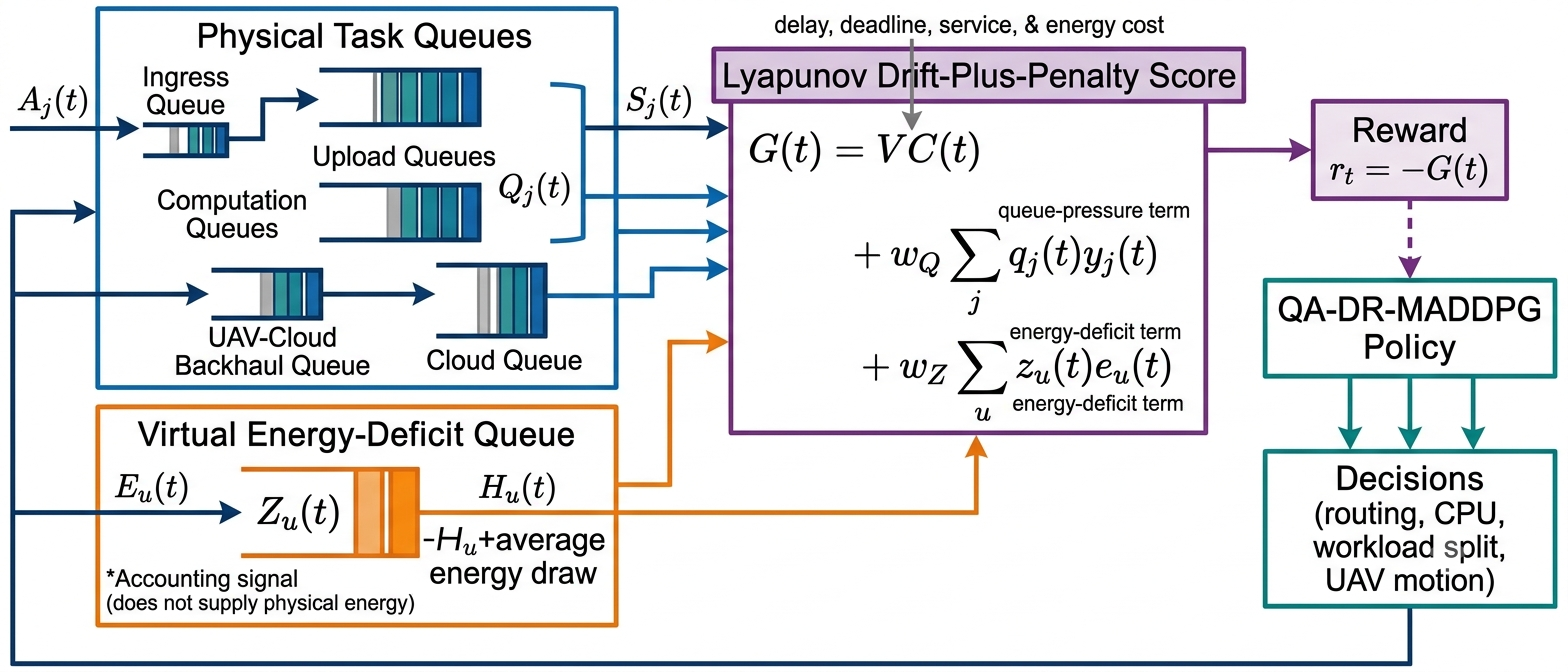
\includegraphics[width=0.94\textwidth]{Physical and virtual queue feedback diagram.png}
\caption{Queue-aware Lyapunov feedback behind the common reward. The
physical task queues and the virtual net-energy deficit both enter the
drift-plus-penalty score, and its negative is passed to the cooperative
controller as the reward. The decisions that are executed then set the queue
service and the energy spent in the next transition.}
\label{fig:lyapunov_feedback}
\end{figure*}

\subsection{Hybrid MADDPG Decision Engine}
The full architecture, with centralized training and decentralized
execution, is drawn in Fig.~\ref{fig:controller_architecture}. Actors shared
within each role form a joint hybrid proposal. The deterministic feasibility
layer turns it into the action that is executed, and the centralized critics
learn from a replay buffer that stores both.

\begin{figure*}[!t]
\centering
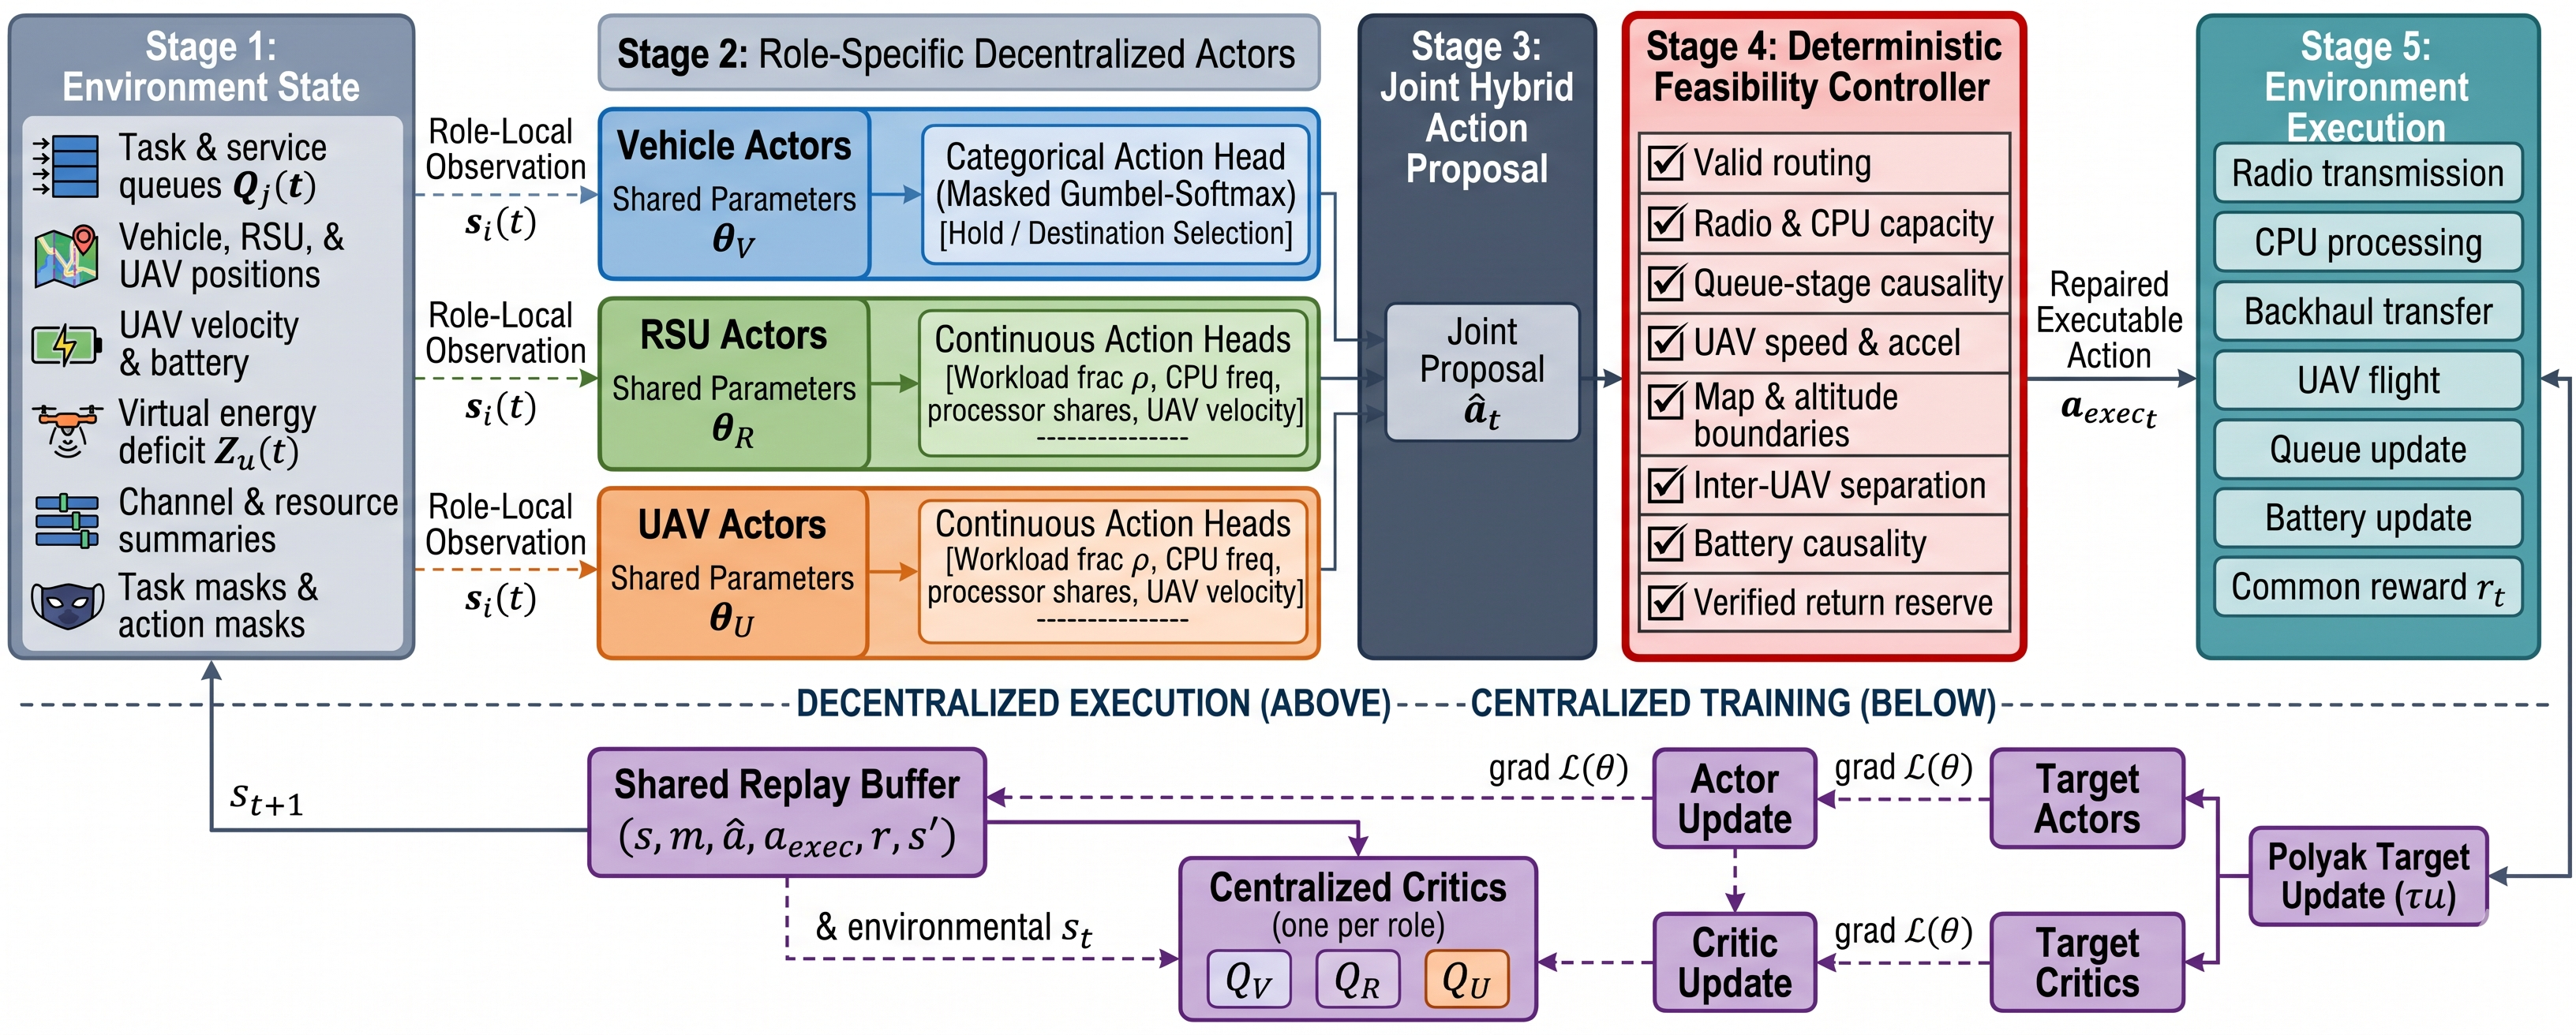
\includegraphics[width=0.98\textwidth]{Complete QA-DR-MADDPG architecture.png}
\caption{Complete \method\ architecture. At execution time, the vehicle,
RSU, and UAV actors rely on role-local observations; the centralized critics
and the shared replay buffer are used only in training. The feasibility
controller sits between the neural proposals and the actions that are
physically executed.}
\label{fig:controller_architecture}
\end{figure*}

\subsubsection{Role-Shared Actors and Centralized Critics}
Each visible task has a feature vector $x_{hi}$ and a mask
$m_{hi}\in\{0,1\}$. The actor passes them through a task encoder followed by
masked pooling:
\begin{align}
e_{hi}&=\phi_g(x_{hi}),\qquad
\bar e_h=\frac{\sum_i m_{hi}e_{hi}}
{\max\{1,\sum_i m_{hi}\}},\nonumber\\
z_h&=\operatorname{LN}\!\left(
\phi_g^{\rm trunk}([o_h;\bar e_h])\right).
\label{eq:actor_encoder}
\end{align}
Parameters are shared by the actors of one role, but different roles have
separate parameters. Each role also has its own centralized critic, which
computes
\begin{equation}
Q_{\psi_g}(s_t,\vect a_t)=q_{\psi_g}([s_t;\operatorname{vec}(\vect a_t)]).
\label{eq:centralized_critic}
\end{equation}

\subsubsection{Categorical and Continuous Action Heads}
Let $l_{hd}$ be the logit of destination $d$ and $c_{hd}$ its feasibility
mask. Choices that are not valid get the logit $-\infty$. In training, the
straight-through Gumbel-softmax output is
\begin{align}
\tilde l_{hd}&=\begin{cases}l_{hd},&c_{hd}=1,\\-\infty,&c_{hd}=0,\end{cases}
\nonumber\\
y_{hd}&=\frac{\exp((\tilde l_{hd}+g_{hd})/\tau_G)}
{\sum_{d'}\exp((\tilde l_{hd'}+g_{hd'})/\tau_G)},\nonumber\\
\hat x_h^{\rm cat}&=\operatorname{sg}
\left(\operatorname{onehot}(\arg\max_d y_{hd})-y_h\right)+y_h,
\label{eq:gumbel_action}
\end{align}
with $g_{hd}=-\log[-\log u_{hd}]$ and $u_{hd}\sim\mathcal U(0,1)$. At
evaluation time there is no Gumbel noise, and the destination is the masked
argmax. The continuous heads are
\begin{align}
\rho_i&=\sigma(z_i^\rho),
&f_u&=f_u^{\max}\sigma(z_u^f),\nonumber\\
\hat{\vect u}_u&=\mathcal S_u\tanh(z_u^{\rm mot}),
&w_{hi}&=\frac{m_{hi}e^{z_{hi}^w}}{\sum_jm_{hj}e^{z_{hj}^w}}.
\label{eq:continuous_heads}
\end{align}
These forms keep the partition fraction and the frequency bounded, keep each
motion component within its configured limit even before physical repair,
and make the positive task shares add up to one.

\subsubsection{Feasibility Controller}
The candidate set $\mathcal C(s_t,\hat a_t)$ holds the proposal itself,
scaled versions of its motion, and the verified contingencies. From it, the
executable action is chosen as
\begin{equation}
a_t^{\rm exec}=\mathcal H(s_t,\hat a_t)
\in\arg\min_{a\in\mathcal C(s_t,\hat a_t)\cap\mathcal F(s_t)}
D(a,\hat a_t),
\label{eq:feasibility_projection}
\end{equation}
where the distance $D$ combines the disagreement in the categorical choices
with the normalized distance between the continuous values. Membership in the
feasible set requires the routing masks, radio and CPU capacity, stage
causality, the speed and acceleration limits, the map and altitude limits,
separation along the continuous path, battery causality, and the return
reserve to be respected. When normal service is not admissible, the UAV stops
accepting new work and follows a verified return or landing contingency. We
keep a record of how proposals differ from the executed actions and of how
often repairs occur, and use both in the evaluation.

\begin{figure*}[!t]
\centering
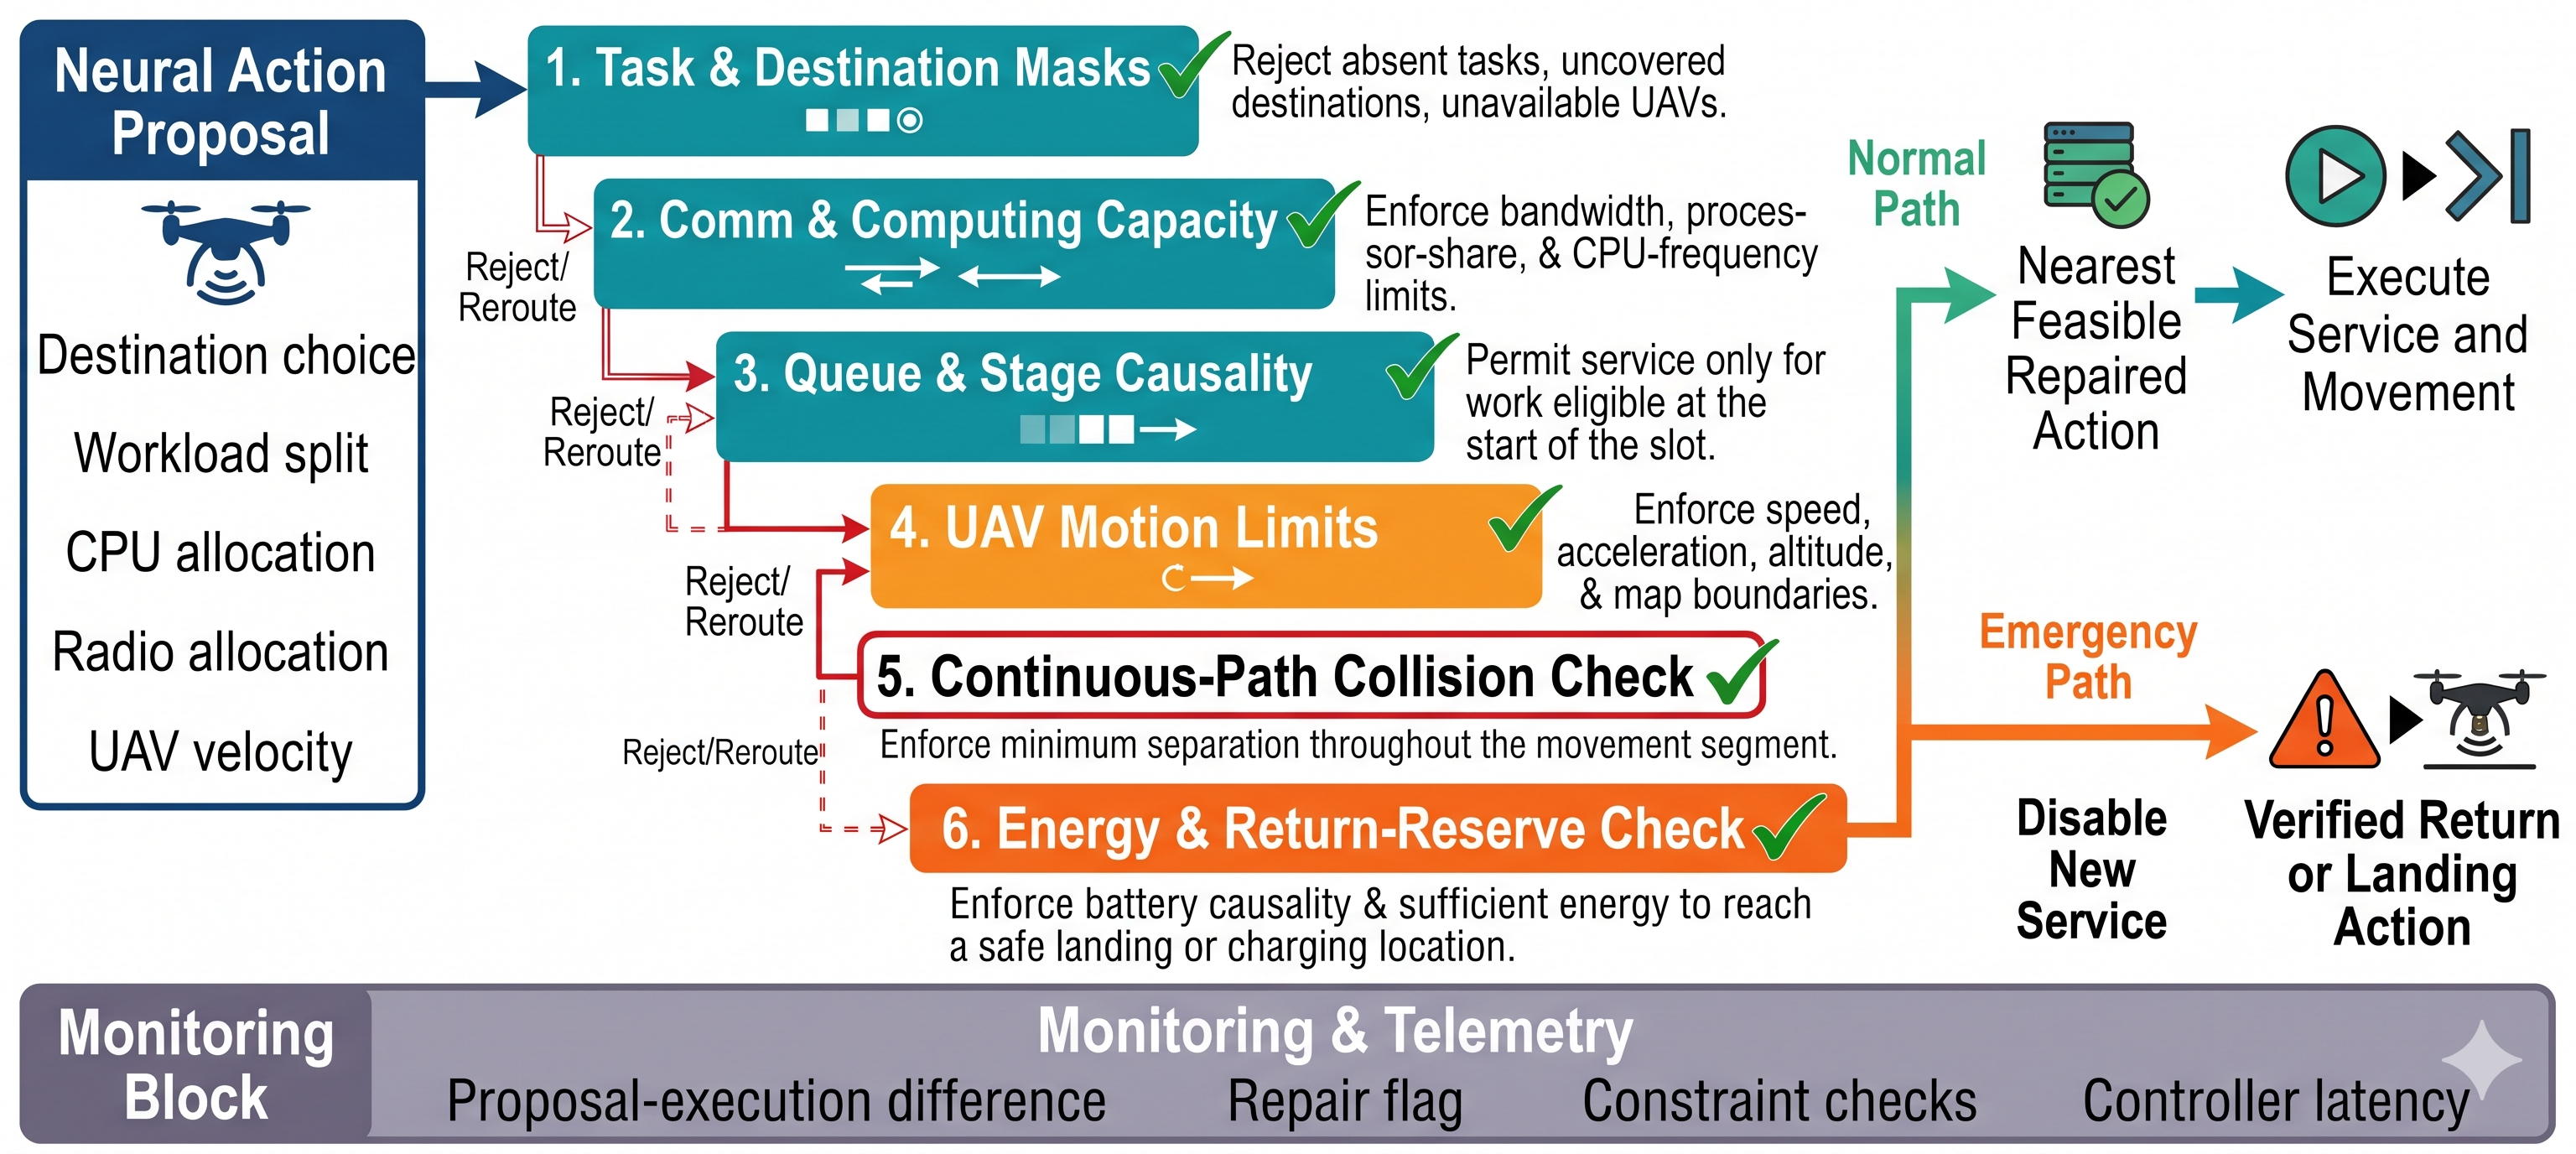
\includegraphics[width=0.95\textwidth]{Feasibility controller and safe-action workflow.png}
\caption{Workflow of the deterministic feasibility controller. Each hybrid
proposal from the networks is tested against the routing, resource,
queue-causality, motion, continuous-path separation, battery, and
return-reserve constraints. The controller then either executes the closest
admissible repair or triggers a verified return or landing contingency.}
\label{fig:feasibility_workflow}
\end{figure*}

\subsubsection{Critic, Actor, and Target Updates}
Each replay entry holds the current and next states, the role observations,
the masks, the proposed and executed joint actions, the reward, and the done
flag $d_b$. For a minibatch of size $B$, the target and the critic loss are
\begin{align}
y_{g,b}&=r_b+\gamma(1-d_b)Q_{\psi_g^-}
(s'_b,\mathcal H_{\rm tens}(\vect a'_b)),\label{eq:critic_target_new}\\
\mathcal L_g(\psi_g)&=\frac1B\sum_{b=1}^{B}
\left(Q_{\psi_g}(s_b,a_b^{\rm exec})-y_{g,b}\right)^2.
\label{eq:critic_loss_new}
\end{align}
When the actor of role $g$ is updated, its current proposal is combined with
the executed replay actions of the other roles, which are detached from the
gradient. Writing $\tilde a_b^{(g)}$ for this mixed action, the actor
maximizes
\begin{equation}
J_g=\frac1B\sum_bQ_{\psi_g}(s_b,\tilde a_b^{(g)})
-\lambda_{\rm rep}\frac1B\sum_b
\|\hat a_{g,b}-\operatorname{sg}(a_{g,b}^{\rm exec})\|_2^2.
\label{eq:actor_objective_new}
\end{equation}
The repair term pulls proposals toward actions that can really be executed.
We do not differentiate through the full physical controller. Following the
Adam updates, the target networks are moved by
\begin{equation}
\theta_g^-\leftarrow(1-\tau_p)\theta_g^-+\tau_p\theta_g,
\qquad
\psi_g^-\leftarrow(1-\tau_p)\psi_g^-+\tau_p\psi_g.
\label{eq:polyak_new}
\end{equation}
In the configuration we report, one actor--critic update is made after every
environment transition as soon as the replay buffer holds 64 samples or more.

\subsection{Domain-Randomized Training and Deployment}
In the completed study, a scenario domain is the tuple
\begin{equation}
\omega=(\lambda,H,C^{\rm bh},\xi),
\label{eq:domain_tuple_correct}
\end{equation}
in which $\lambda$ sets the load or a change in traffic, $H$ selects nominal,
zero, or interrupted replenishment, $C^{\rm bh}$ is the backhaul capacity,
and $\xi$ is the recorded random seed for tasks and harvesting. There are
$10\times7=70$ scenario specifications in the training manifest. In each
epoch, seven different specifications are drawn from it uniformly and
without replacement. In expectation, every declared stress class is seen
equally often, although a given epoch need not contain an example of each
class.

We train for the robust objective
\begin{equation}
\max_\Theta\;\E_{\omega\sim p_{\rm train}}
\E_{\tau\sim\pi_\Theta,\omega}
\left[\sum_{t=0}^{T-1}\gamma^t r_t\right].
\label{eq:dr_objective_new}
\end{equation}
Every episode updates the same parameters $\Theta$. No task-specific copies
are made, and there is no Reptile interpolation. Validation is done on 35
separate specifications (five seeds for each of the seven stresses). A
checkpoint is kept only if it raises the mean validation reward and has zero
modeled physical violations. For early stopping, the patience is ten
validations.

\begin{figure*}[!t]
\centering
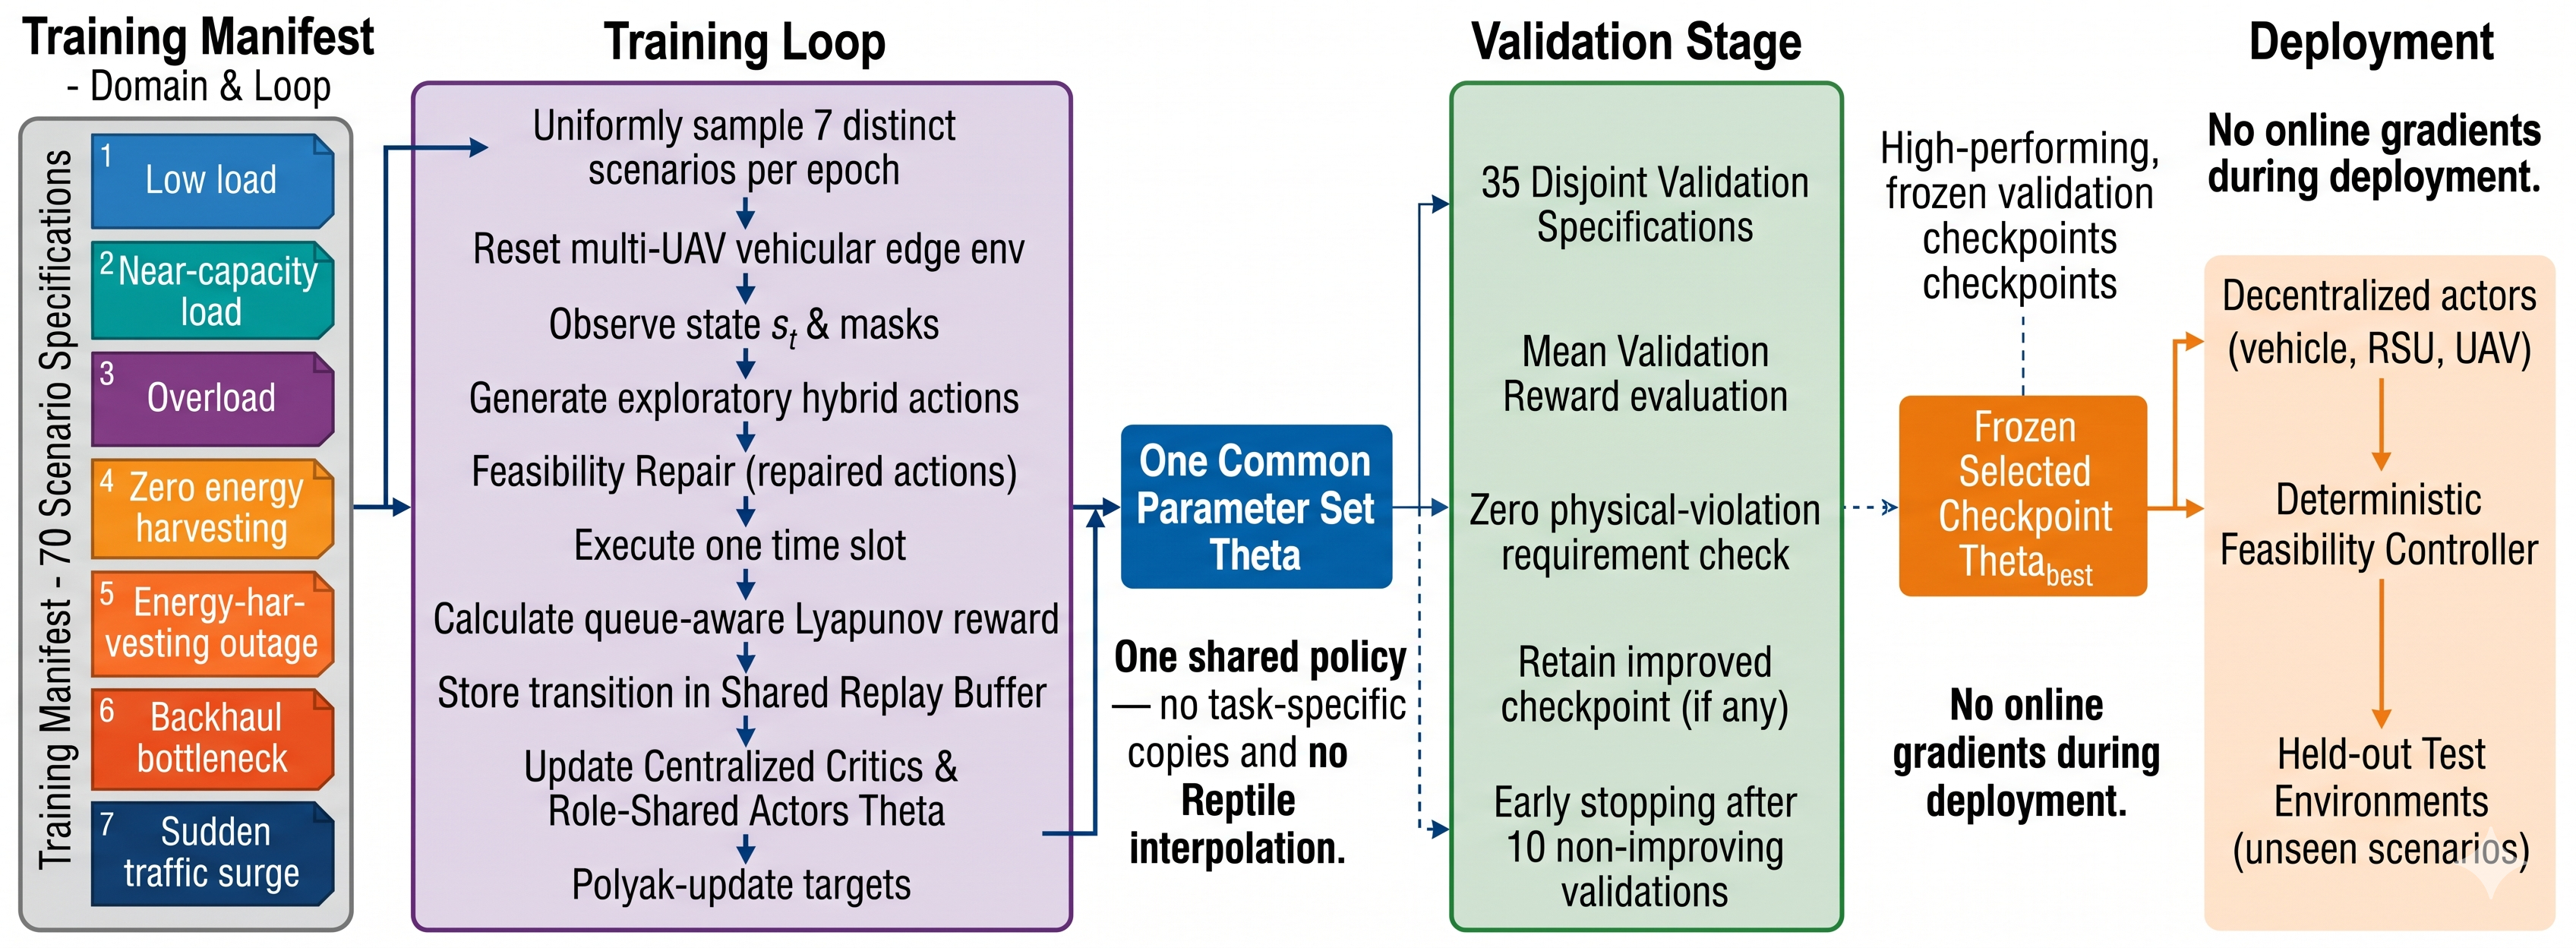
\includegraphics[width=0.98\textwidth]{Domain-randomized training and deployment workflow.png}
\caption{Workflow for domain-randomized training, validation, and
deployment. All seven stress classes update a single shared set of
parameters, and validation on separate data picks an improved checkpoint
with no violations. At deployment, the selected actors are frozen, and the
centralized critics, replay sampling, and gradient updates are switched off.}
\label{fig:dr_workflow}
\end{figure*}

\begin{algorithm}[!t]
\caption{Queue-aware domain-randomized Hybrid MADDPG}
\label{alg:dr_maddpg_new}
\KwIn{Training manifest $\Omega_{\rm tr}$, replay capacity $N$, batch size $B$,
target rate $\tau_p$}
\KwOut{Validation-selected parameters $\Theta^*$}
Initialize online/target actors, critics, and replay $\mathcal D$\;
\For{each epoch $e$}{
 sample seven distinct scenarios $\omega\subset\Omega_{\rm tr}$\;
 \For{each sampled scenario and slot $t$}{
  encode $s_t$, local observations, task masks, and action masks\;
  generate exploratory hybrid proposal $\hat a_t$\;
  execute $a_t^{\rm exec}=\mathcal H(s_t,\hat a_t)$\;
  observe $r_t,s_{t+1}$ and append the complete transition to $\mathcal D$\;
  \If{$|\mathcal D|\ge B$}{
   update all role critics using Eq.~\eqref{eq:critic_loss_new}\;
   update all role actors using Eq.~\eqref{eq:actor_objective_new}\;
   apply Eq.~\eqref{eq:polyak_new}\;
  }
 }
 evaluate the fixed policy on all validation specifications\;
 retain only an improved, zero-violation checkpoint; stop after ten
 non-improving validations\;
}
\end{algorithm}

Once deployed, the controller needs, in each slot, one forward pass through
the role-local actors and then a call to the deterministic feasibility
controller. The selected parameters do not change, since the centralized
critics, replay sampling, and gradient updates are all disabled. What the
evaluation measures, then, is how well the trained policy generalizes to the
test scenarios with no online adaptation.

\subsection{Computational and Storage Complexity}
For role $g$, let $n_g$ be the number of agents, $d_g$ the observation width,
and $a_g$ the action width. We also write $M_{\rm task}$ for the maximum
number of visible tasks, $d_{\rm task}$ for the width of a task feature,
$h_a$ and $h_c$ for the hidden widths of the actor and the critic, $d_s$ for
the width of the global state, and $d_A=\sum_gn_ga_g$. One joint pass
through the actors then costs
\begin{align}
C_\mu=\mathcal O\!\Bigg(\sum_gn_g\big[&
M_{\rm task}(d_{\rm task}h_a+h_a^2)\nonumber\\
&+(d_g+h_a)h_a+h_a^2+h_aa_g\big]\Bigg),
\label{eq:actor_complexity_new}
\end{align}
and with one centralized critic per role, the critic cost is
\begin{equation}
C_Q=\mathcal O\!\left(|\mathcal G|
\left[(d_s+d_A)h_c+h_c^2+h_c\right]\right).
\label{eq:critic_complexity_new}
\end{equation}
A single minibatch update therefore takes $\mathcal O(B(C_\mu+C_Q))$. If the
feasibility repair tries $K_{\rm rep}$ joint candidates, each at cost
$C_{\rm feas}$, it adds at most $\mathcal O(K_{\rm rep}C_{\rm feas})$ per
slot. The replay buffer needs $\mathcal O(Nd_{\rm tr})$ storage, and the
networks, target networks, gradients, and Adam state together need
$\mathcal O(P_\Theta)$. In decentralized deployment no critic is evaluated,
so the cost per slot is $\mathcal O(C_\mu+K_{\rm rep}C_{\rm feas})$.

\iffalse
\section{Proposed \method\ Methodology}
\subsection{Constrained Markov Decision Process}
We formulate the controller as
$\langle\mathcal S,\mathcal A,\mathcal P,\mathcal R,\gamma\rangle$.

\subsubsection{State and Observations}
The centralized state $s_t$ contains vehicle/UAV positions, UAV velocities
and modes, all physical queues, task ages and remaining stages, channel
features, CPU availability, battery fractions, return reserves, virtual
energy queues, harvesting state, and normalized time. Actor $i$ observes only
the role-relevant projection $o_i(t)$, preserving centralized training and
decentralized execution (CTDE).

\subsubsection{Hybrid Action Space}
Vehicle actors choose a masked destination and, where allowed, a partition
fraction. RSU and UAV actors produce processor-sharing weights. UAV actors
also produce CPU frequency and three-dimensional velocity. The joint proposal
is
\begin{equation}
\vect a_t=\{\vect a_v^{\mathrm{route}},\vect a_r^{\mathrm{cpu}},
\vect a_u^{\mathrm{cpu}},\vect a_u^{\mathrm{flight}}\}.
\end{equation}
Categorical logits use a straight-through one-hot estimator during training;
continuous values use bounded output transformations.

\subsubsection{Transition and Reward}
The transition includes task arrivals, mobility, radio and computation
service, queue updates, battery expenditure, harvesting, and safety-state
changes. A common reward is
\begin{equation}
r_t=-G_{\mathrm{DPP}}(t),
\end{equation}
where $G_{\mathrm{DPP}}(t)$ is the normalized drift-plus-penalty score derived
below. Reward uses executed rather than proposed actions.

\subsection{Lyapunov Queue and Energy Transformation}
For long-term target $\bar E_u$, define a virtual deficit queue
\begin{equation}
Z_u(t+1)=\big[Z_u(t)+E_u(t)-\bar E_u\big]^+.
\end{equation}
Using physical and virtual queues, choose
\begin{equation}
L(t)=\frac{1}{2}\left(\sum_q Q_q^2(t)+\sum_u Z_u^2(t)\right).
\end{equation}
The conditional drift is
$\Delta(t)=\E[L(t+1)-L(t)\mid s_t]$. After applying
$([x-y]^++z)^2\le x^2+y^2+z^2+2x(z-y)$, an upper bound has the control-dependent
form
\begin{align}
\Psi(t)=&\sum_q Q_q(t)
\big(A_q(t)+I_q(t)-\mu_q(t)\big)\nonumber\\
&+\sum_u Z_u(t)\big(E_u(t)-\bar E_u\big)+VP(t),\\
\Delta(t)+V\E[P(t)\mid s_t]
\le&\ C+\E[\Psi(t)\mid s_t].
\label{eq:dpp}
\end{align}
The quantity $\Psi(t)$ defines $G_{\mathrm{DPP}}(t)$. Large physical queues
increase the value of service, whereas a large virtual deficit increases the
cost of UAV energy. $V$ controls the delay--energy trade-off.

\subsection{Hybrid MADDPG Decision Engine}
For role $g$, actor $\mu_{\theta_g}$ maps local observation and action masks
to a proposal. A centralized critic
$Q_{\psi_g}(s,\vect a)$ observes the joint state and joint executed action.
Target networks generate the temporal-difference target
\begin{equation}
y_g=r+\gamma(1-d)Q_{\psi_g^-}
\left(s',\vect a'\right),
\end{equation}
where $d$ marks termination or truncation and $\vect a'$ is repaired by the
tensor-level action map. Critic loss is
\begin{equation}
\mathcal L_g(\psi_g)=\frac{1}{B}\sum_{b=1}^B
\left(Q_{\psi_g}(s_b,\vect a_b^{\mathrm{exec}})-y_{g,b}\right)^2.
\end{equation}
The deterministic actor update is
\begin{equation}
\nabla_{\theta_g}J_g\approx\frac{1}{B}\sum_{b=1}^B
\nabla_{a_g}Q_{\psi_g}(s_b,\vect a_b)
\nabla_{\theta_g}\mu_{\theta_g}(o_{g,b}).
\end{equation}
Target parameters use Polyak averaging
\begin{equation}
\theta_g^-\leftarrow\tau\theta_g+(1-\tau)\theta_g^-,\qquad
\psi_g^-\leftarrow\tau\psi_g+(1-\tau)\psi_g^-.
\end{equation}

\subsection{Feasibility Controller}
Before execution, the controller masks unavailable destinations, normalizes
processor shares, clamps frequencies, projects motion into the admissible
flight region, searches collision-free joint motion candidates, and checks
battery and verified return reserve. The environment recomputes service and
energy from the repaired action. Replay stores both proposed and executed
actions so that the critic learns the actual transition. All learned methods
use the same feasibility controller.

\subsection{Domain-Randomized Training Phase}
A domain
\begin{equation}
\omega=(\lambda,\mathcal C,H,C^{\mathrm{bh}},\mathcal M)
\end{equation}
contains offered-load statistics $\lambda$, channel conditions $\mathcal C$,
harvesting process $H$, backhaul capacity $C^{\mathrm{bh}}$, and mobility/task
trace $\mathcal M$. At each episode,
\begin{equation}
\omega_e\sim p_{\mathrm{train}}(\omega).
\end{equation}
The robust objective is
\begin{equation}
\max_\Theta\;\E_{\omega\sim p_{\mathrm{train}}}
\E_{\tau\sim\pi_\Theta,\omega}
\left[\sum_{t=0}^{T-1}\gamma^tr_t\right].
\label{eq:dr_objective}
\end{equation}
Unlike Reptile, all episodes update the same parameters $\Theta$; there are no
task-specific copies or outer parameter interpolation. Validation uses
disjoint seeds and selects only checkpoints with zero modeled physical
violations.

\begin{algorithm}[!t]
\caption{Queue-aware domain-randomized Hybrid MADDPG}
\label{alg:dr_maddpg}
\KwIn{Training-domain distribution $p_{\mathrm{train}}$, replay capacity
$N$, batch size $B$, update rate $\tau$}
\KwOut{Validation-selected policy parameters $\Theta^*$}
Initialize online and target actors/critics and replay $\mathcal D$\;
\For{each training epoch}{
  sample scenarios $\omega_e\sim p_{\mathrm{train}}(\omega)$\;
  \For{each slot $t$ in each sampled scenario}{
    observe $s_t$ and role observations $\{o_i(t)\}$\;
    generate masked hybrid proposal $\vect a_t$ with exploration\;
    execute $\vect a_t^{\mathrm{exec}}=\mathcal H(s_t,\vect a_t)$\;
    observe $r_t,s_{t+1}$ and store transition in $\mathcal D$\;
    \If{$|\mathcal D|\ge B$}{
      sample a minibatch and update centralized critics\;
      update role actors through the critics\;
      Polyak-update all target networks\;
    }
  }
  evaluate on fixed validation scenarios\;
  retain a checkpoint only if it improves reward and remains feasible\;
}
\end{algorithm}

\subsection{Execution and Complexity Analysis}
At deployment, only decentralized actors and the deterministic feasibility
controller execute. No online gradients are required. For an $L$-layer MLP
with widths $h_0,\ldots,h_L$, forward complexity is
\begin{equation}
C_{\mathrm{MLP}}=\mathcal O\left(\sum_{\ell=1}^{L}h_{\ell-1}h_\ell\right).
\end{equation}
With $G$ role actors, $G$ critics, batch size $B$, $U$ updates per slot,
$E$ episodes, and $T$ slots, training complexity is
\begin{equation}
\mathcal O\left(ET\left[C_{\mathrm{env}}+UB
\left(C_{\mathrm{actor}}+C_{\mathrm{critic}}\right)\right]\right).
\end{equation}
Replay storage is $\mathcal O(Nd_{\mathrm{tr}})$ for transition width
$d_{\mathrm{tr}}$. Domain randomization changes scenario generation but does
not add a Reptile inner/outer loop.
\fi

\section{Numerical Results}
\subsection{Simulation Configuration}
All settings of the frozen research-v1 study are listed in
Tables~\ref{tab:sim}--\ref{tab:domains}. We used scenario-generation seeds
$0$--$9$ for training, $100$--$104$ for validation and $200$--$209$ for
testing, with learner seeds $0$--$4$. The test split contains ten paired
scenario traces for each of seven stress classes, so the five learned methods
give $5\times5\times70=1{,}750$ runs in the comparisons below. Our archived
evaluation actually holds 3,150 runs; the extra ones come from four
non-learning integration baselines that fall outside the learned-controller
comparison.

In this benchmark the vehicles sit at static synthetic positions and every
node has a fixed uplink capacity. The simulator does implement the
geometry-aware channel and the recorded-mobility interface of Section~III,
but neither was enabled for these results. What follows is therefore
evidence of robustness to the declared variations in traffic, harvesting,
outages, backhaul and stochastic traces. Robustness to channel or mobility
changes was not tested.

\begin{table*}[!t]
\caption{Physical, Workload, and Energy Parameters of the Reported Benchmark}
\label{tab:sim}
\centering
\footnotesize
\begin{tabular}{p{0.22\textwidth}p{0.21\textwidth}p{0.22\textwidth}p{0.21\textwidth}}
\toprule
Parameter & Value & Parameter & Value\\
\midrule
Area; slot duration & $1000\times1000$ m$^2$; 1 s & Vehicles; RSUs; UAVs & 3; 2; 2\\
Offered-load/drain horizon & 200/100 slots & Vehicle CPU & $0.5$ GHz each\\
RSU/UAV/cloud CPU & $3/2/12$ GHz & RSU/UAV uplink & $20/12$ Mbit/s each\\
Nominal/bottleneck backhaul & $20/0.5$ Mbit/s & UAV altitude; speed & 50--150 m; 20 m/s\\
Climb/descent; acceleration & 5/5 m/s; 10 m/s$^2$ & Minimum separation & 50 m\\
Battery capacity/initial charge & 50/45 kJ & Mean harvest & 140 J/slot, $\pm20\%$\\
Task input; CPU cycles & 2--6 Mbit; 3.2--4.8 Gcycle & Deadline; partitionable ratio & 8--20 s; 0.5\\
Blade/induced hover power & 79.86/88.63 W & Rotor-tip/induced speed & 120/4.03 m/s\\
UAV compute coefficient $\kappa$ & $10^{-28}$ & UAV RX/BH/control power & 2/5/1 W\\
Vehicle transmit power & 0.4 W & Queue/energy reference & $10^9$ cycles/$10^3$ J\\
Lyapunov $V,w_Q,w_Z$ & 1, 1, 1 & Maximum visible tasks & 16 per actor\\
\bottomrule
\end{tabular}
\end{table*}

\begin{table}[!t]
\caption{Learning Configuration}
\label{tab:learning_config}
\centering
\footnotesize
\begin{tabular}{p{0.48\columnwidth}p{0.40\columnwidth}}
\toprule
Parameter & Value\\
\midrule
Actor/critic hidden width & 128/256\\
Actor/critic learning rate & $10^{-3}/10^{-3}$\\
Discount/Polyak rate & 0.99/0.01\\
Batch/replay/warm-up & 64/$10^5$/64\\
Gradient updates per slot & 1 after warm-up\\
Exploration standard deviation/decay & 0.15/0.995\\
Scenarios sampled per epoch & 7 of 70 train specifications\\
Validation specifications & 35 per validation\\
Maximum epochs/early-stop patience & 50/10 validations\\
Independent learner seeds & 5\\
Training device & CPU\\
\bottomrule
\end{tabular}
\end{table}

\begin{table}[!t]
\caption{Declared Domain Conditions}
\label{tab:domains}
\centering
\footnotesize
\begin{tabular}{p{0.34\columnwidth}p{0.56\columnwidth}}
\toprule
Condition & Parameterization\\
\midrule
Low load & Offered-load ratio 0.35\\
Near capacity & Offered-load ratio 0.85\\
Overload & Offered-load ratio 1.25\\
Zero harvest & $H_u(t)=0$ for all slots\\
Harvest outage & 140 J mean except slots 66--132\\
Backhaul bottleneck & $C^{\rm bh}=0.5$ Mbit/s\\
Traffic surge & Load ratio 0.35 to 1.25 at slot 100\\
Nominal conditions & 20 Mbit/s backhaul; 140 J mean harvest\\
\bottomrule
\end{tabular}
\end{table}

\subsection{Compared Learned Controllers and Metrics}
We compare five learned controllers: nominal Hybrid MADDPG, the proposed
\method, Reptile-MADDPG, Reptile-MADDPG with the physical-queue weighting
removed, and Hybrid MAPPO. Since all of them are learned, the differences
come from training and policy family, and a handcrafted heuristic cannot
take credit for policy quality. A task counts toward deadline success if it
finishes before its relative deadline; completion counts late tasks as well.
Throughput is completed tasks per second. Final backlog is measured once the
100-slot drain has ended, reward is summed over the full trace, and system
energy counts each ownership component a single time. Controller latency,
action repair and physical violations are reported separately.

Statistics are computed at the level of learner seeds. For every
independently trained seed the paired test scenarios are averaged first, and
the 95\% Student-$t$ intervals are built from these five values. Evaluating a
checkpoint on more traces would not increase the number of independent
training repetitions.

The direct queue-weight ablation was run as a separate experiment. Using the
same five learner seeds, the domain-randomized controller is trained with and
without physical-queue weighting, and each checkpoint is tested on 70 paired
specifications ($2\times5\times70=700$ frozen runs). These checkpoints were
retrained independently of the full benchmark, so we only interpret paired
differences inside this study and do not place its absolute means next to
those of Table~\ref{tab:overall}.

\subsection{Learning Behaviour}
Fig.~\ref{fig:learning} plots the validation reward of every learner seed for
the proposed method and for the three main training baselines. In
Fig.~\ref{fig:learning_mean} all five learned techniques appear together:
each early-stopped run is rescaled to normalized training progress and the
five seeds are averaged. Hybrid MADDPG and \method\ generally end at a higher
validation reward than the two Reptile variants, and the Reptile curves are
more spread out between seeds. This supports evaluating a fixed
domain-randomized policy. It says nothing about few-shot adaptation.

\begin{figure*}[!t]
\centering
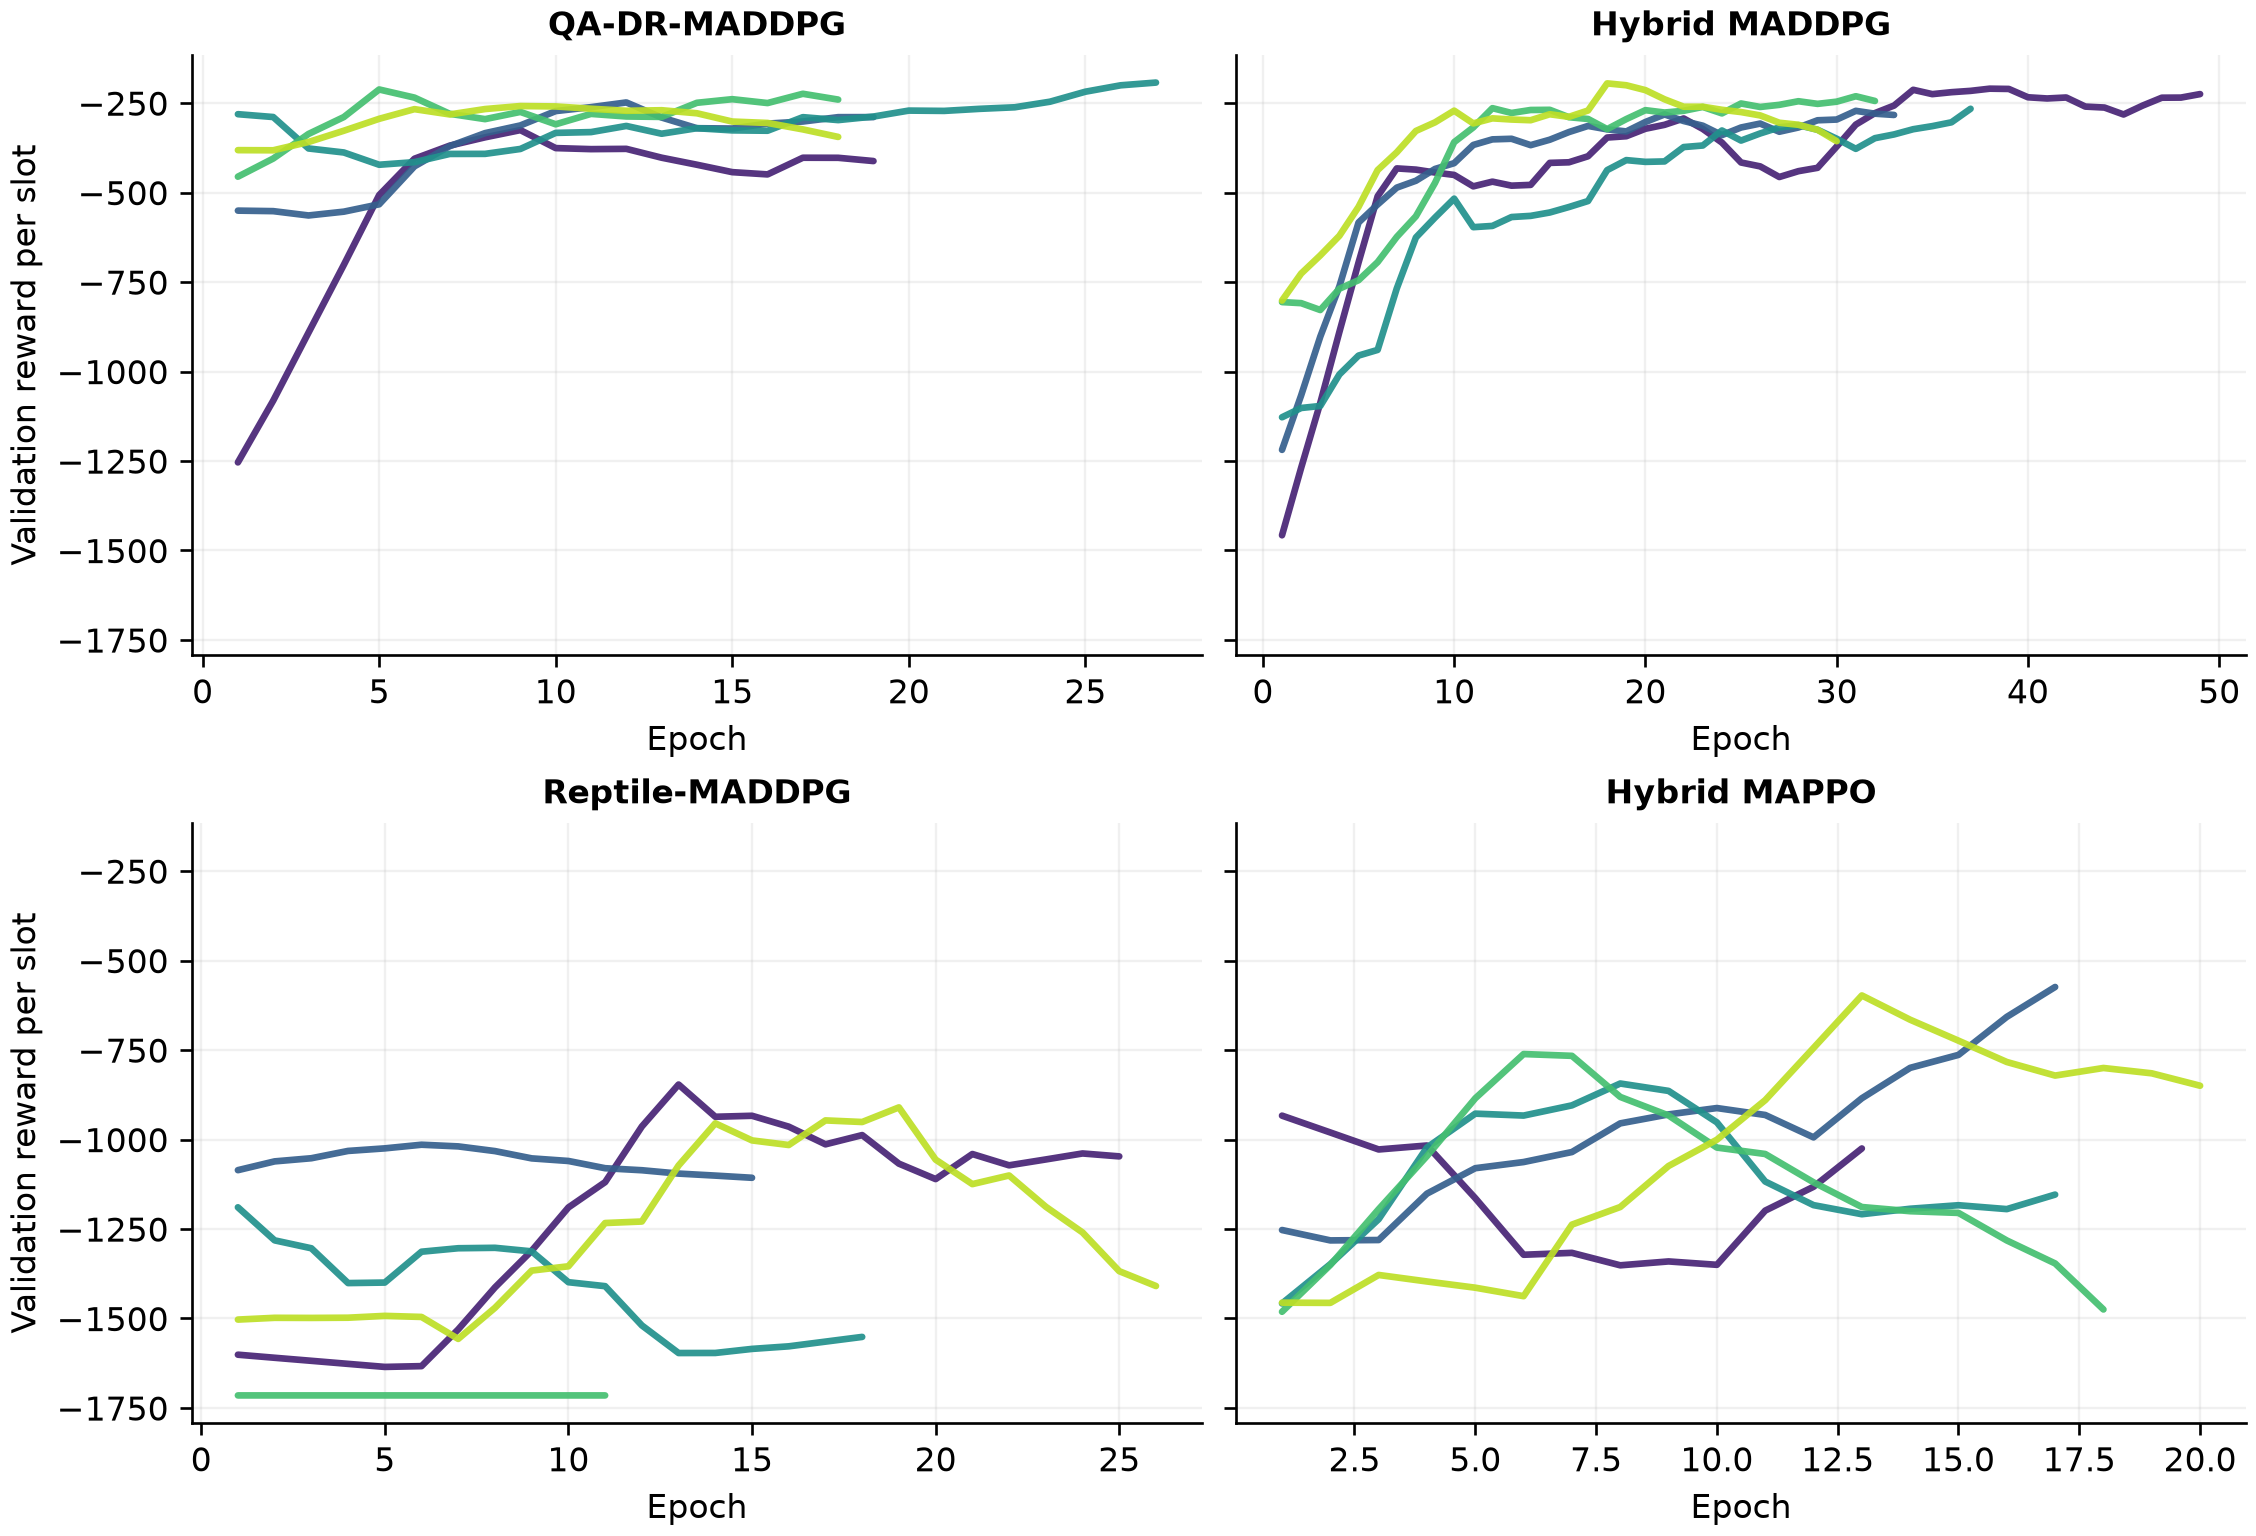
\includegraphics[width=0.95\textwidth]{learning_curves_learned_methods.png}
\caption{Validation learning curves for the proposed method, nominal Hybrid
MADDPG, Reptile-MADDPG and Hybrid MAPPO, with one line per independent
learner seed. A short centered moving average is applied only so that the
trend of each seed is easier to follow.}
\label{fig:learning}
\end{figure*}

\begin{figure*}[!t]
\centering
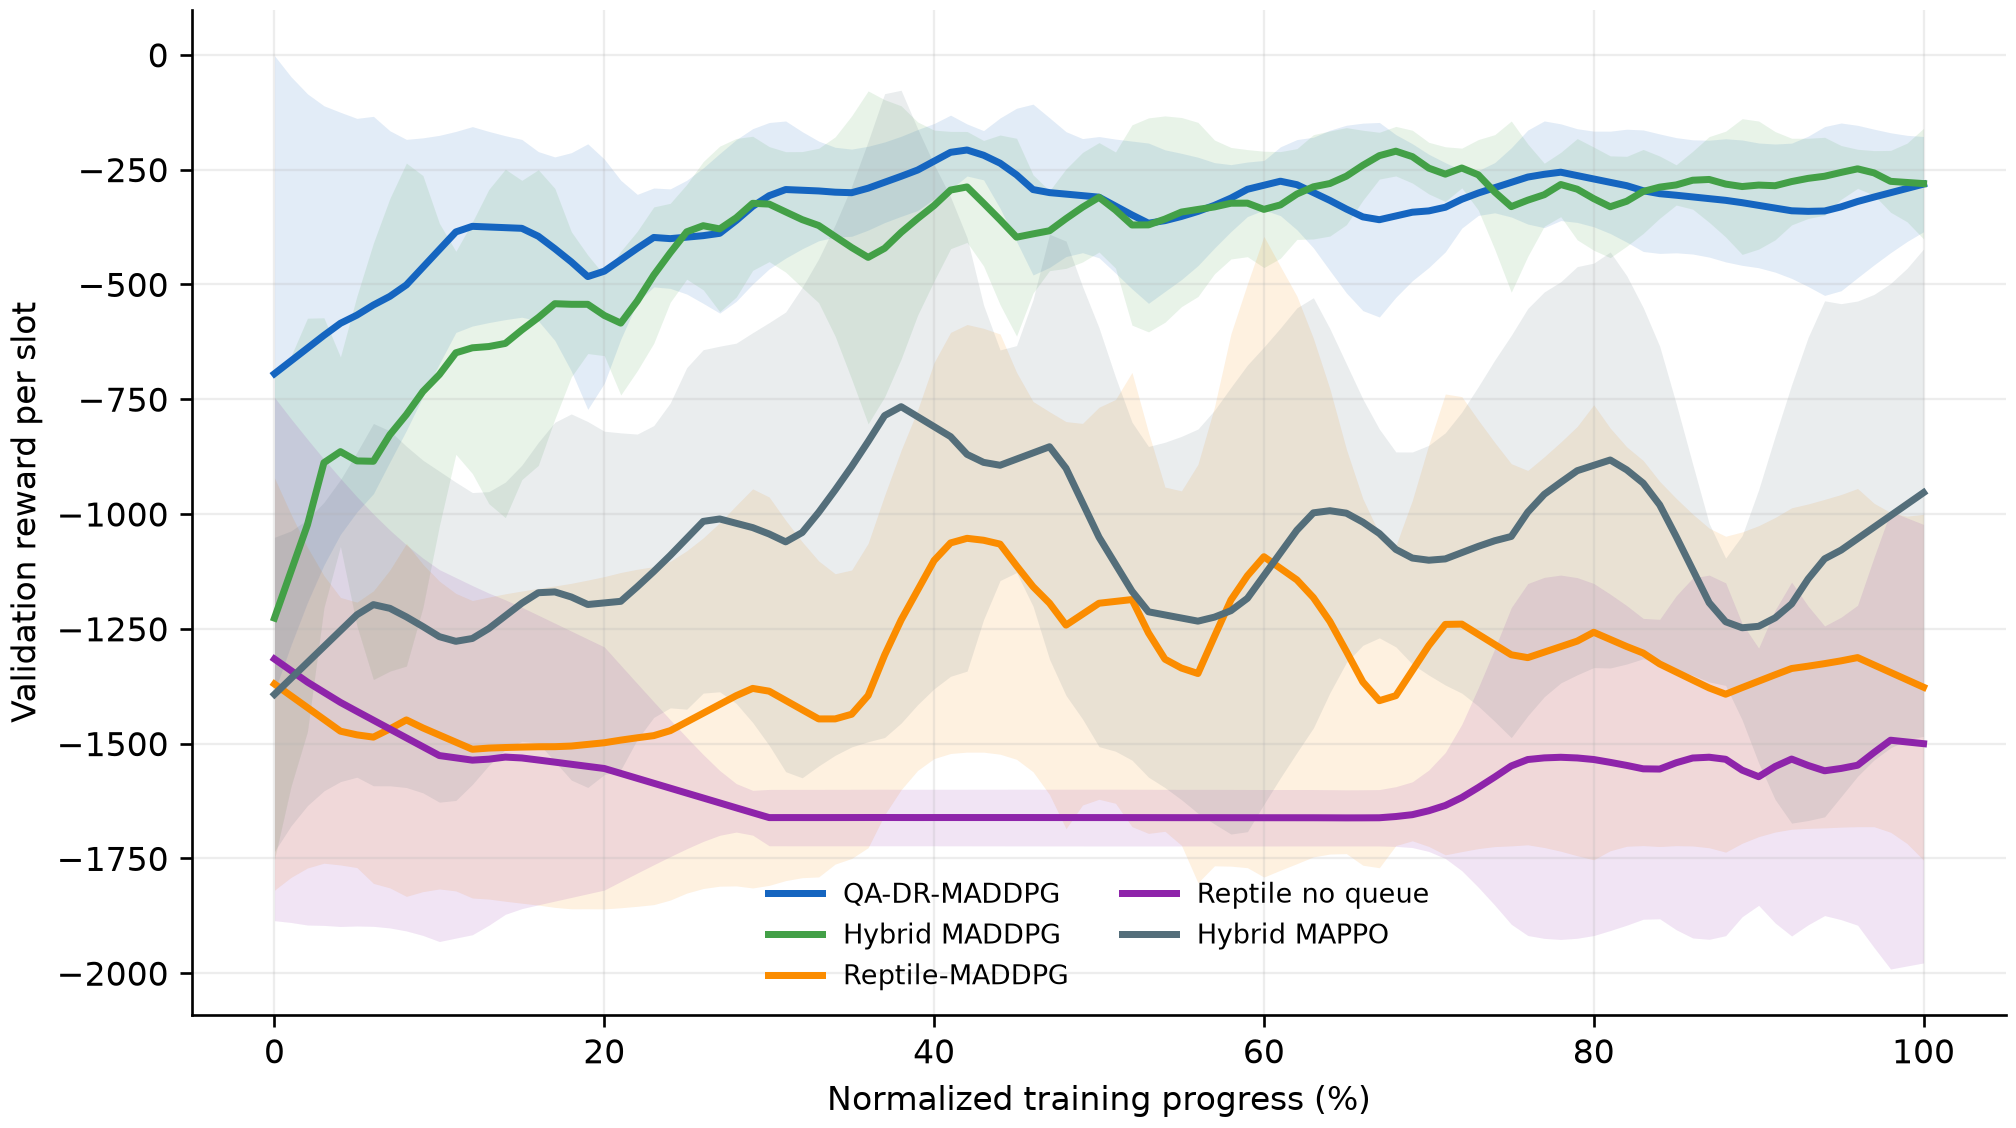
\includegraphics[width=0.88\textwidth]{validation_reward_mean_all_methods.png}
\caption{Mean validation reward per slot for all learned techniques, plotted
against normalized training progress because early stopping gives the runs
different epoch counts. Solid lines average the five independent learner
seeds; shaded bands are 95\% Student-$t$ confidence intervals.}
\label{fig:learning_mean}
\end{figure*}

\subsection{Overall Service and Energy Performance}
Table~\ref{tab:overall} and Fig.~\ref{fig:overall} give the test results.
Among the learned controllers, \method\ has the highest completion rate
(81.96\%) and throughput (0.914 tasks/s) and the best cumulative reward
($-48.3\times10^3$). On numerical deadline success Hybrid MAPPO is marginally
ahead, at 42.41\% against 41.50\%. Reptile-MADDPG spends the least energy,
but it completes only 59.07\% of tasks and ends with $5.58\times10^{11}$
cycles of backlog, so its low energy figure reflects reduced service more
than efficiency.

\begin{table*}[!t]
\caption{Learner-Seed Mean Performance Across Held-Out Stress Conditions}
\label{tab:overall}
\centering
\footnotesize
\begin{tabular}{lrrrrrr}
\toprule
Method & Deadline (\%) & Completion (\%) & Throughput & Reward & Backlog (Gcycle) & Energy (kJ)\\
\midrule
Hybrid MADDPG & 22.16 & 77.93 & 0.847 & $-52{,}076$ & 206.9 & 18.15\\
\textbf{\method} & 41.50 & \textbf{81.96} & \textbf{0.914} & \textbf{$-48{,}292$} & 250.1 & 19.06\\
Reptile-MADDPG & 32.17 & 59.07 & 0.600 & $-271{,}616$ & 557.9 & \textbf{8.70}\\
Reptile no queue & 15.95 & 48.71 & 0.451 & $-333{,}804$ & 728.2 & 39.74\\
Hybrid MAPPO & \textbf{42.41} & 76.75 & 0.827 & $-125{,}162$ & 278.3 & 13.61\\
\bottomrule
\end{tabular}
\end{table*}

\begin{figure*}[!t]
\centering
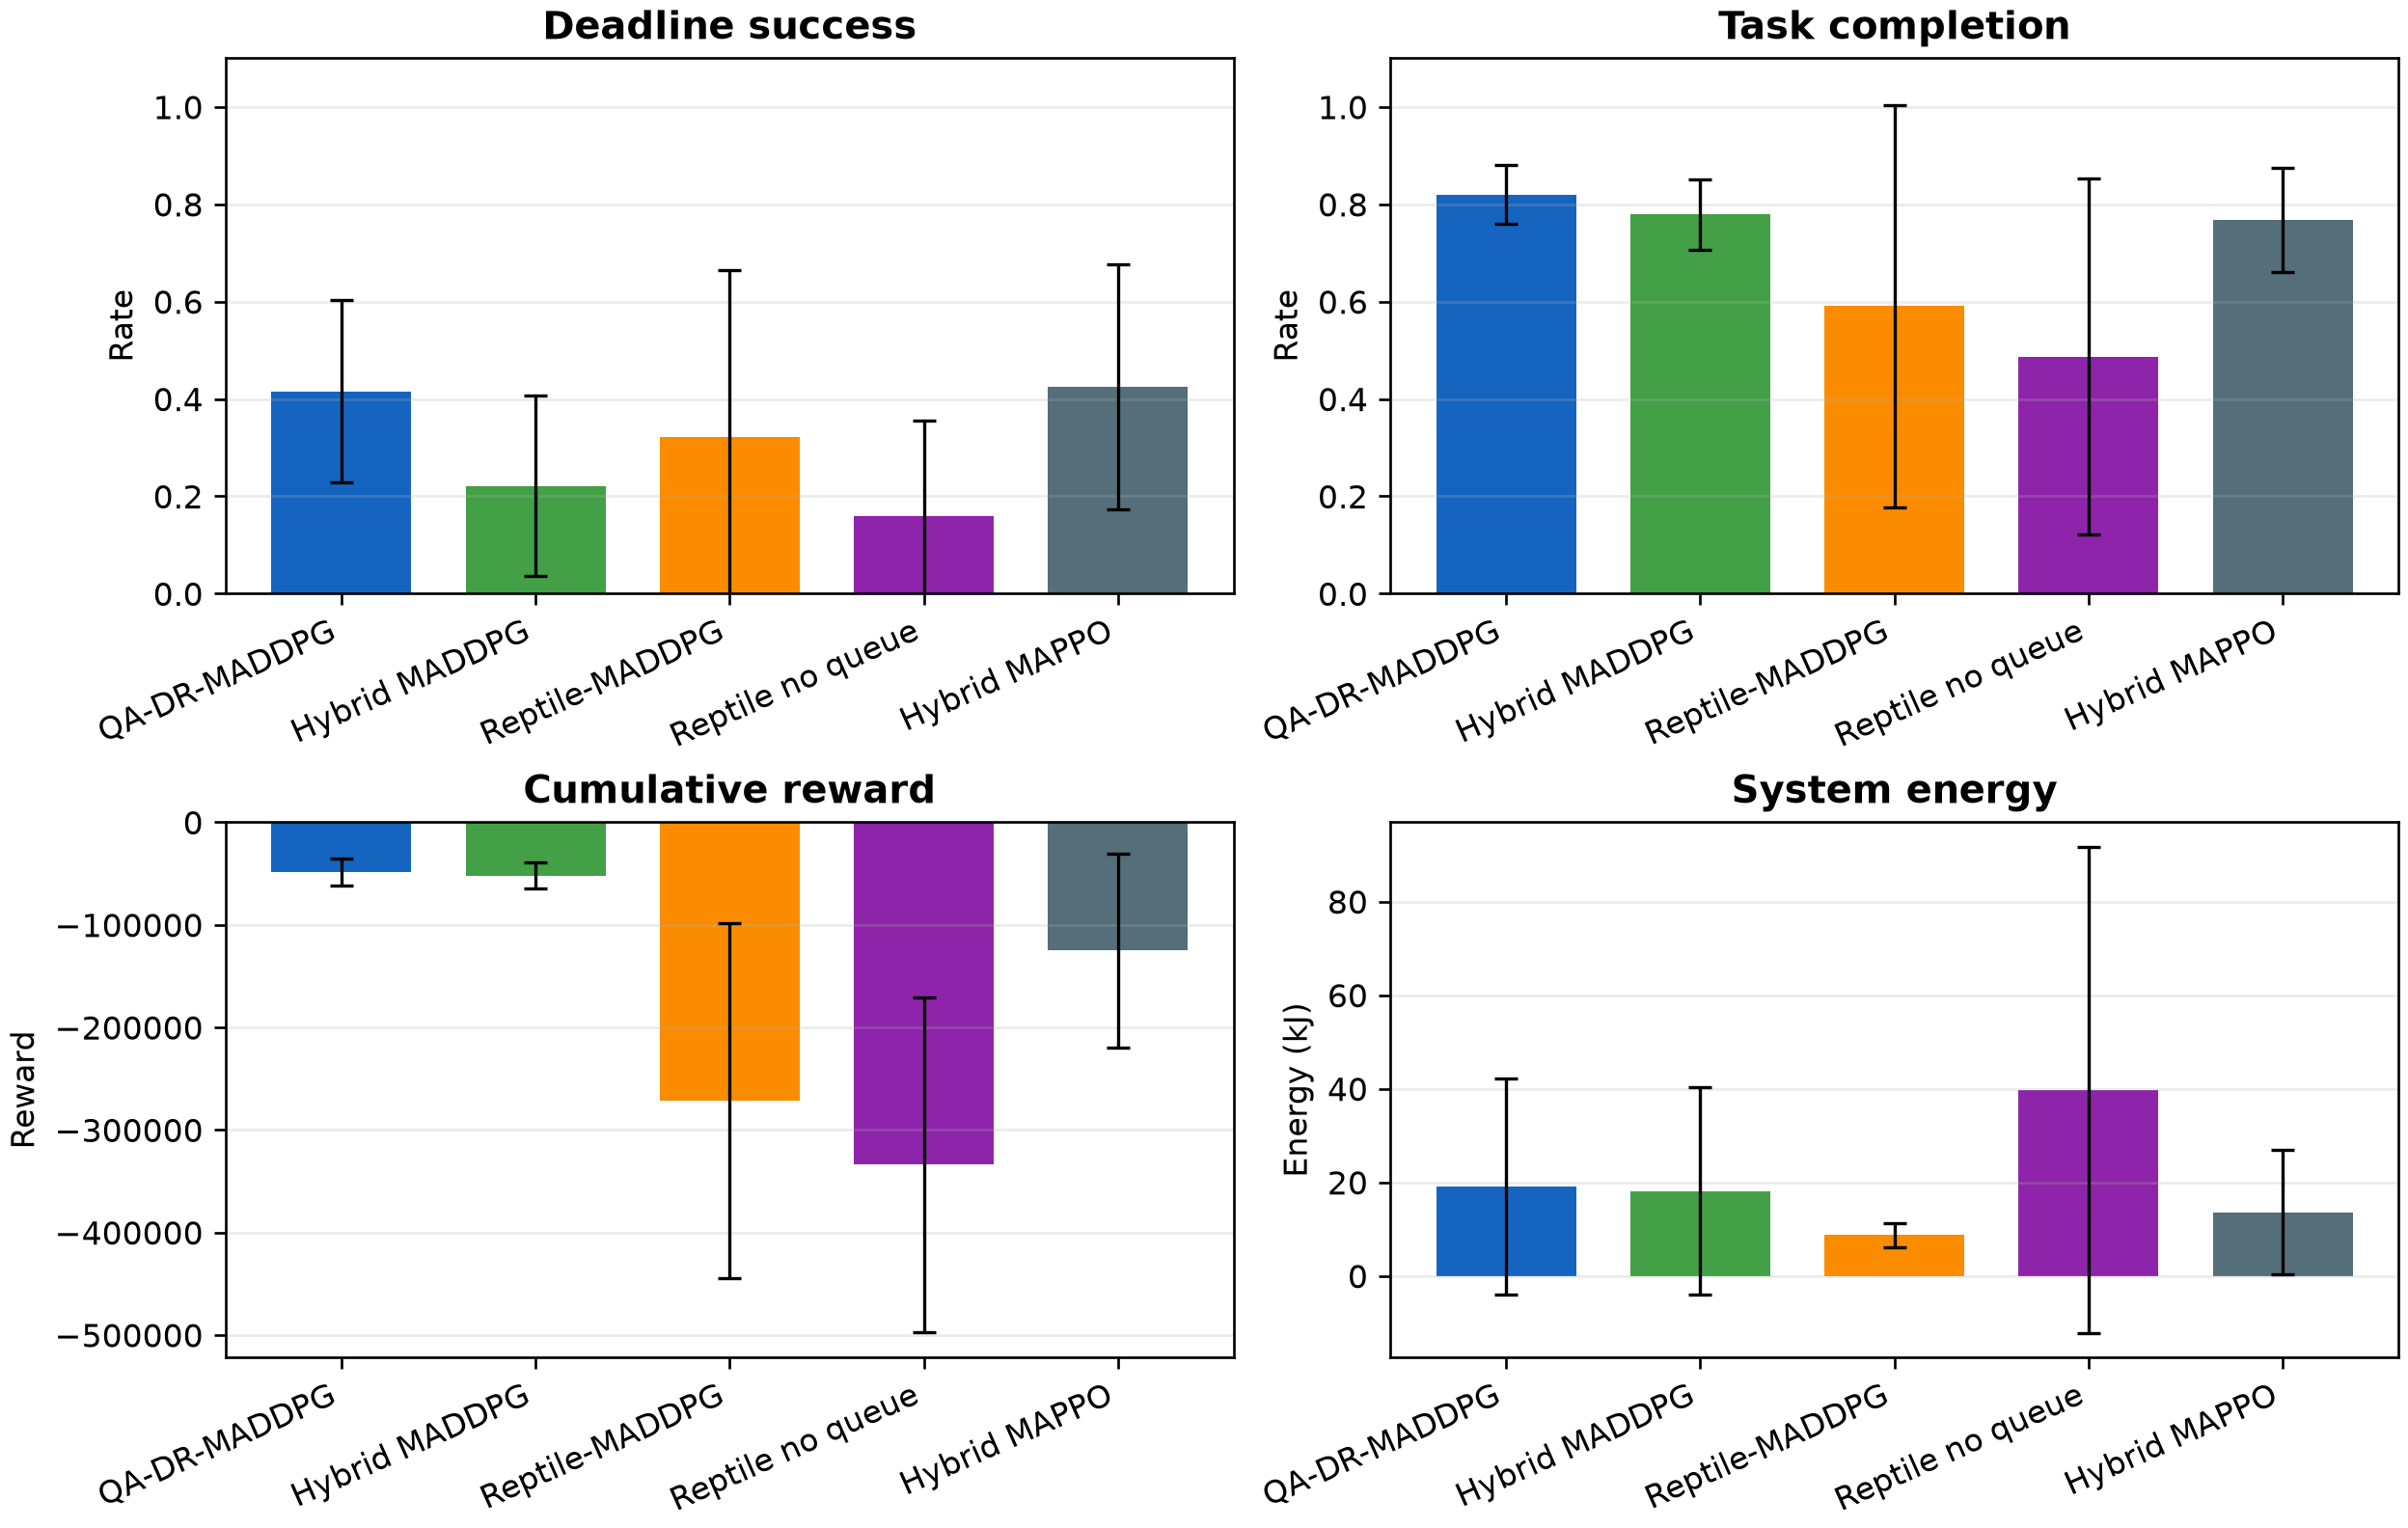
\includegraphics[width=0.92\textwidth]{overall_learned_methods.png}
\caption{Overall performance of the learned controllers. Read the energy
panel together with completion and backlog: a policy can save energy just by
keeping its UAVs unavailable. Error bars are 95\% Student-$t$ intervals over
five independent learner seeds.}
\label{fig:overall}
\end{figure*}

\subsection{Robustness Across Stress Conditions}
Looking at the conditions one at a time, \method\ completes about 99.8\% of
tasks at light load, under the harvesting changes and under backhaul
degradation, and MAPPO also does well in these regimes. Near capacity and in
overload, all learned methods lose ground. In overload, completion drops to
about 46.6\% for Hybrid MADDPG, 37.7\% for \method, 29.7\% for MAPPO and
19.9\% for Reptile-MADDPG. Randomized training improves generalization across
conditions, but it cannot add service capacity that the modeled network
lacks.

The average over conditions also hides some regime-specific behaviour.
Nominal Hybrid MADDPG completes more tasks than \method\ in overload, and the
ranking reverses only when we average over the full declared stress family.
The gain from domain randomization is a gain in that cross-condition average,
not in every single case.

\subsection{Sensitivity to Offered Load}
Fig.~\ref{fig:load_sensitivity} isolates the three completed experiments in
which the nominal offered-load ratio goes from 0.35 to 0.85 and then 1.25,
while topology, processor capacities, nominal harvesting and backhaul stay
fixed. The proposed method has the lowest numerical p95 response time at low
load and the best reward per slot in overload. At the two higher loads,
however, nominal Hybrid MADDPG ends with less backlog. Once the offered work
nears or exceeds the available service capacity, both methods degrade
sharply.

Because response-time percentiles include only completed tasks, they need to
be read next to the final backlog. In overload, a controller may report a
lower percentile simply because its slowest tasks never finished and were
censored from the latency sample. Reward per slot is the cumulative reward
divided by the 300-slot evaluation length shared by all runs (200
offered-load slots followed by 100 drain slots). One learner seed of each
Reptile variant finished no tasks at these loads. We leave its p95 response
time undefined instead of imputing a value, but the seed stays in the backlog
and reward panels.

\begin{figure*}[!t]
\centering
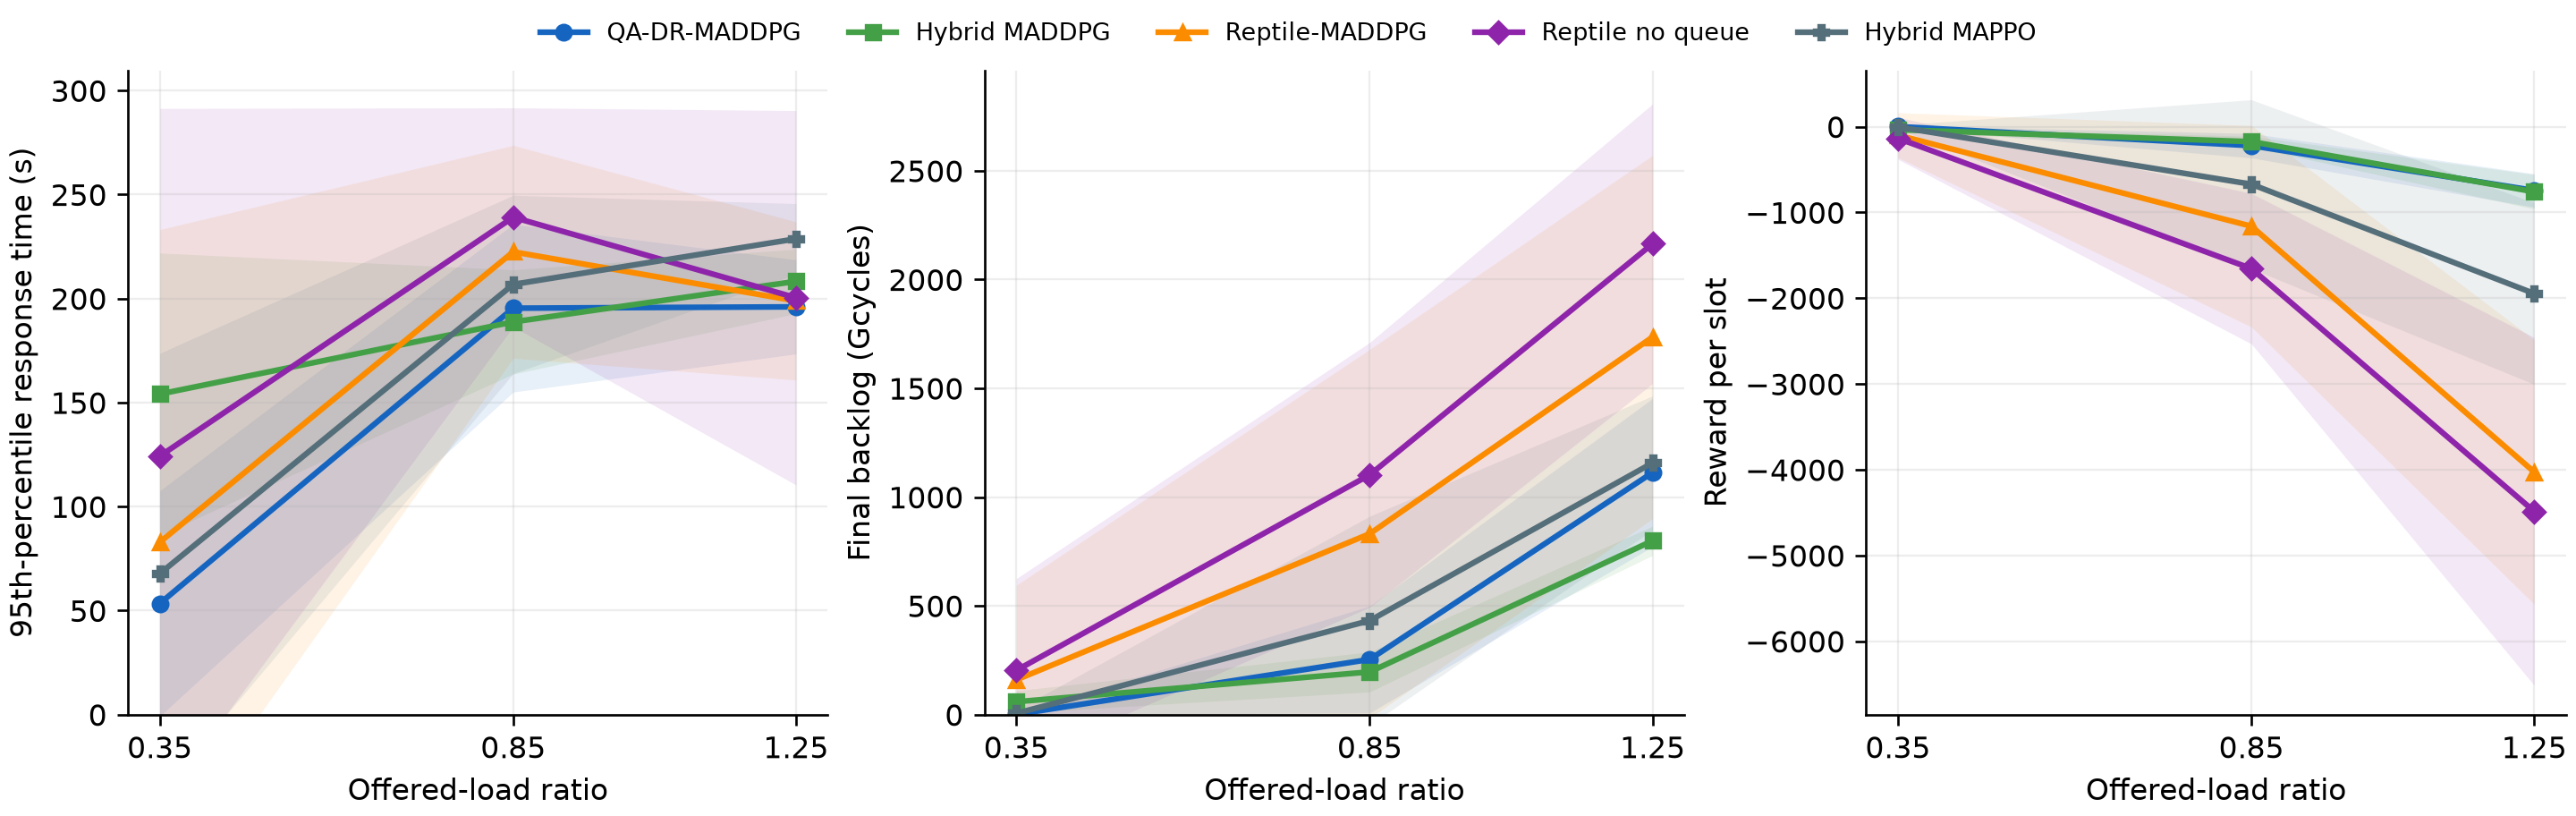
\includegraphics[width=0.98\textwidth]{offered_load_sensitivity.png}
\caption{Offered-load sensitivity of the five learned controllers. Lines show
learner-seed means and shaded regions 95\% Student-$t$ confidence intervals.
Backlog and reward use all five independently trained seeds. The p95
response time is taken over completed tasks; the two Reptile variants have
only four usable seeds here because the fifth completed no tasks, while the
other latency curves use all five. Final backlog includes unfinished work.}
\label{fig:load_sensitivity}
\end{figure*}

\subsection{Domain-Randomization Ablation}
Hybrid MADDPG and \method\ use the same hybrid actor--critic family and the
same feasibility layer. The only difference is the training distribution: the
former sees the nominal domain alone, the latter samples all declared
training domains. According to Table~\ref{tab:dr_ablation}, randomization
adds 19.34 percentage points of numerical deadline success, 4.03 points of
completion, 0.067 tasks/s of throughput and 3,784 of reward. It also costs
0.91 kJ more energy and leaves 43.2 Gcycles more backlog. Every five-seed
paired confidence interval for these differences includes zero, so we treat
them as numerical improvements and not as statistically established ones.

\begin{table}[!t]
\caption{Domain-Randomization Ablation}
\label{tab:dr_ablation}
\centering
\footnotesize
\resizebox{\columnwidth}{!}{%
\begin{tabular}{lrrp{0.34\columnwidth}}
\toprule
Metric & Hybrid & \method & Paired $\Delta$ [95\% CI]\\
\midrule
Deadline success & 0.222 & 0.415 & $+0.193$ [$-0.072,0.459$]\\
Completion & 0.779 & 0.820 & $+0.040$ [$-0.028,0.109$]\\
Throughput (task/s) & 0.847 & 0.914 & $+0.067$ [$-0.095,0.230$]\\
Reward & $-52{,}076$ & $-48{,}292$ & $+3{,}784$ [$-15{,}924,23{,}492$]\\
Backlog (Gcycle) & 206.9 & 250.1 & $+43.2$ [$-25.2,111.6$]\\
Energy (kJ) & 18.15 & 19.06 & $+0.91$ [$-35.07,36.89$]\\
\bottomrule
\end{tabular}
}
\end{table}

\begin{figure}[!t]
\centering
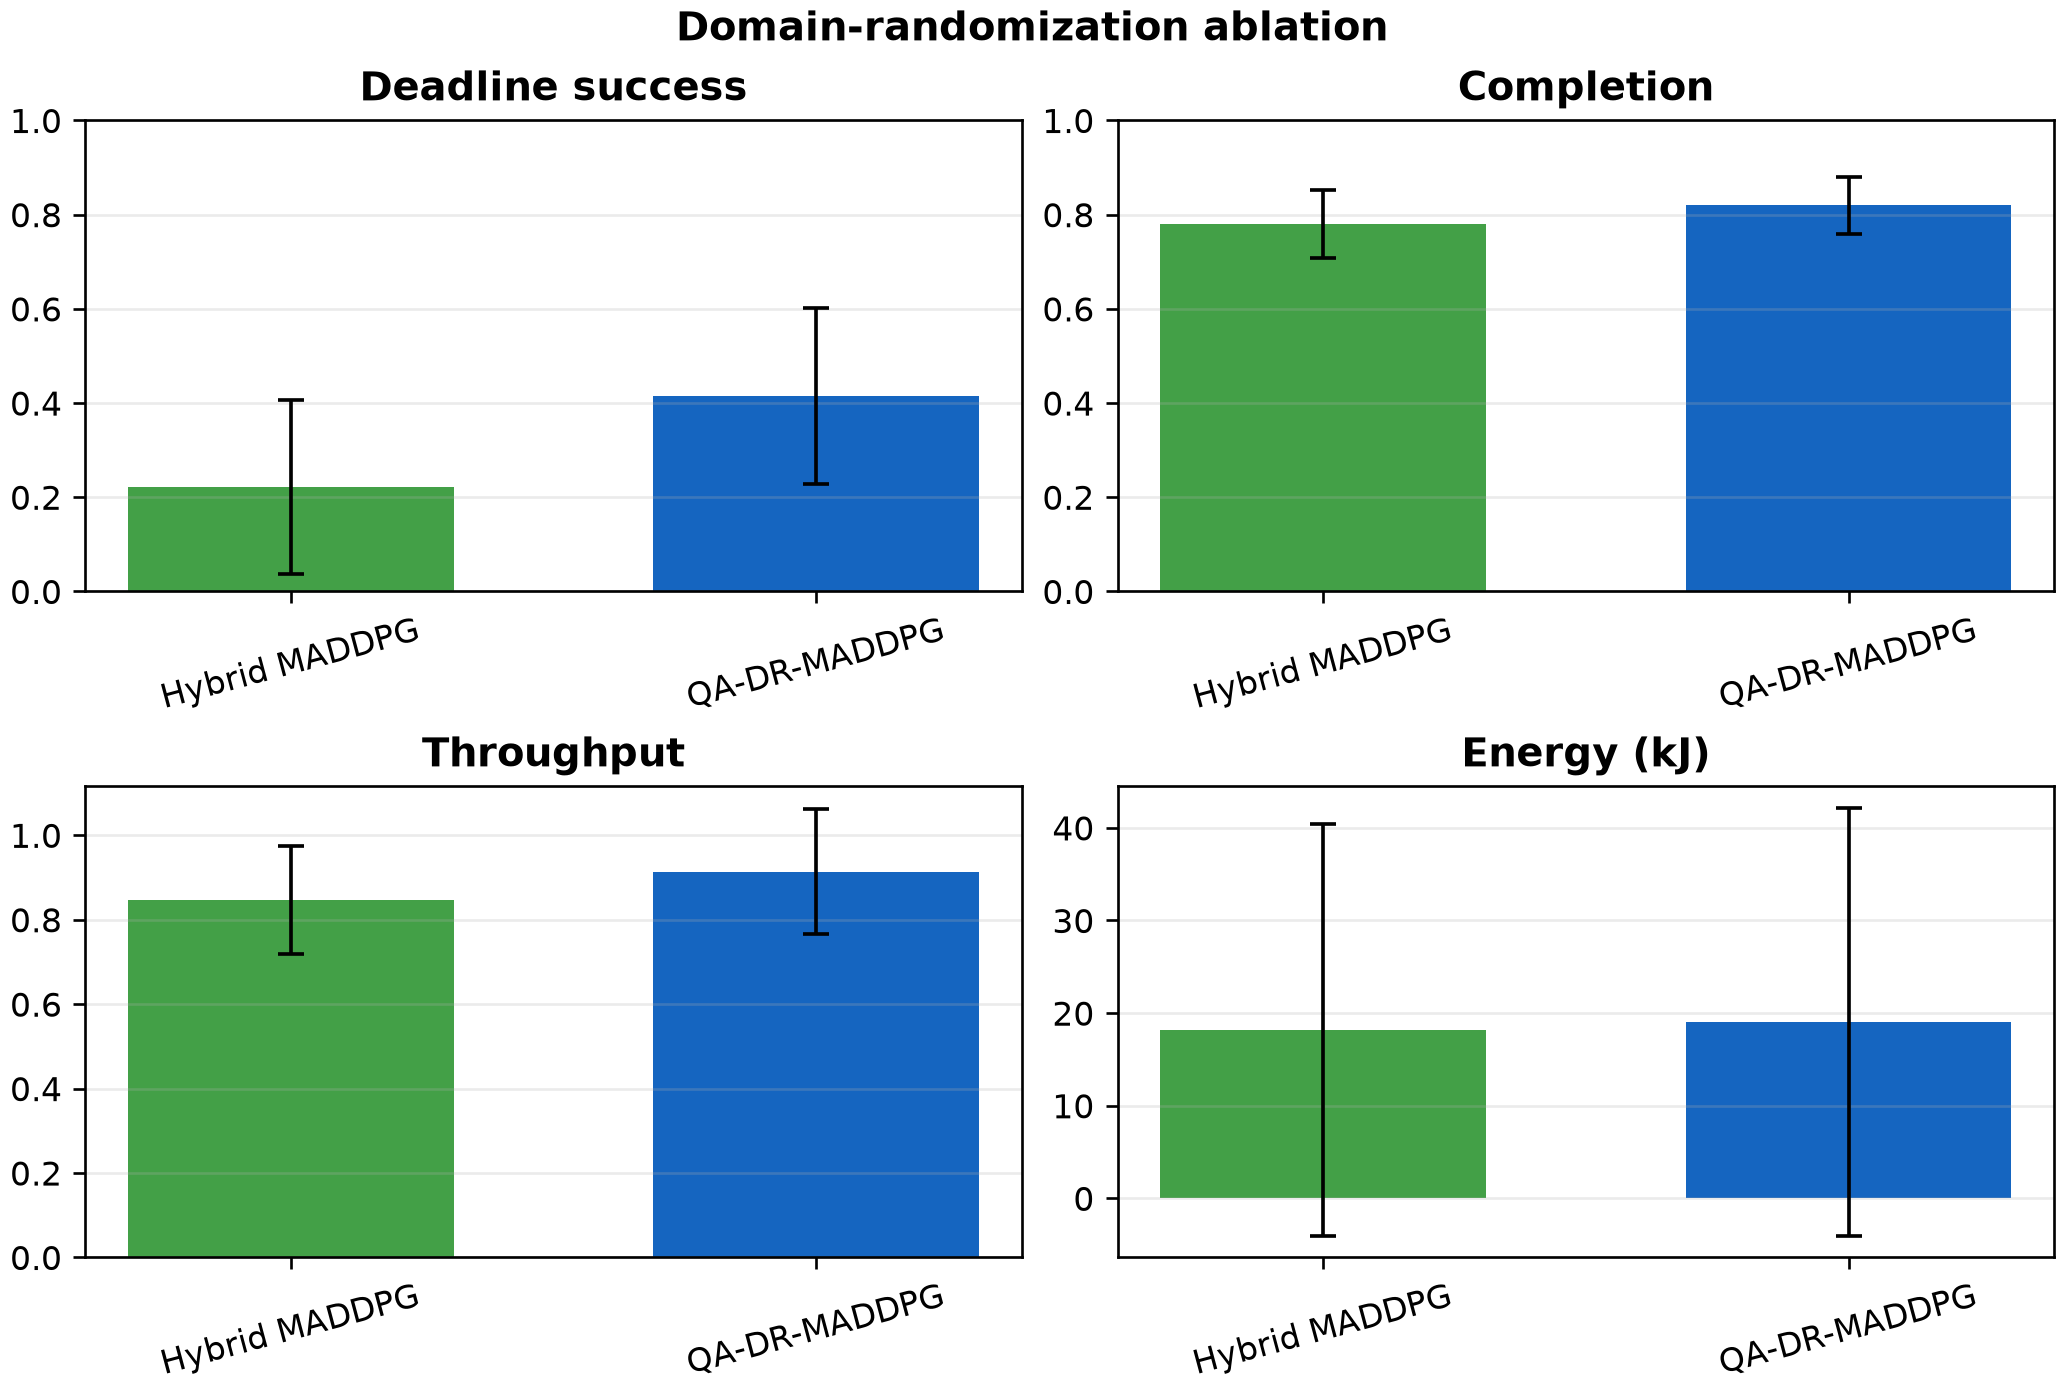
\includegraphics[width=\columnwidth]{domain_randomization_ablation.png}
\caption{Nominal Hybrid MADDPG compared with the domain-randomized proposed
method. Error bars are 95\% Student-$t$ intervals over five learner seeds;
Table~\ref{tab:dr_ablation} lists the paired-difference intervals.}
\label{fig:dr_ablation}
\end{figure}

\subsection{Direct Physical-Queue-Weight Ablation}
Here the proposed domain-randomized MADDPG backbone is trained twice with
paired learner seeds, once with the physical-queue terms in the Lyapunov
reward and once without them. Architecture, domain sampling, training, safety
and evaluation settings are otherwise identical. With queue weighting,
average deadline success rises by 16.17 percentage points, completion by
31.42 points, throughput by 0.470 tasks/s and reward by 241,982, while final
backlog falls by 467.0 Gcycles (Table~\ref{tab:queue_ablation}). The paired
95\% confidence intervals for throughput, backlog and reward exclude zero.
Deadline success and completion improve as well, but with only five
independent learner seeds their intervals still include zero. System energy
moves by just 0.66 kJ, again with an interval that includes zero, so the
service gain should not be read as an established energy reduction.

\begin{table}[!t]
\caption{Direct Physical-Queue-Weight Ablation of Domain-Randomized MADDPG}
\label{tab:queue_ablation}
\centering
\footnotesize
\resizebox{\columnwidth}{!}{%
\begin{tabular}{lrrp{0.31\columnwidth}}
\toprule
Metric & No queue & Queue-aware & Paired $\Delta$ [95\% CI]\\
\midrule
Deadline success & 0.180 & 0.342 & $+0.162$ [$-0.050,0.373$]\\
Completion & 0.515 & 0.829 & $+0.314$ [$-0.033,0.661$]\\
Throughput (task/s) & 0.428 & 0.898 & $+0.470$ [$0.053,0.887$]\\
Reward & $-294{,}956$ & $-52{,}974$ & $+241{,}982$ [$70{,}906,413{,}059$]\\
Backlog (Gcycle) & 668.2 & 201.2 & $-467.0$ [$-829.6,-104.4$]\\
Energy (kJ) & 10.32 & 10.97 & $+0.66$ [$-2.92,4.23$]\\
\bottomrule
\end{tabular}
}
\end{table}

\begin{figure}[!t]
\centering
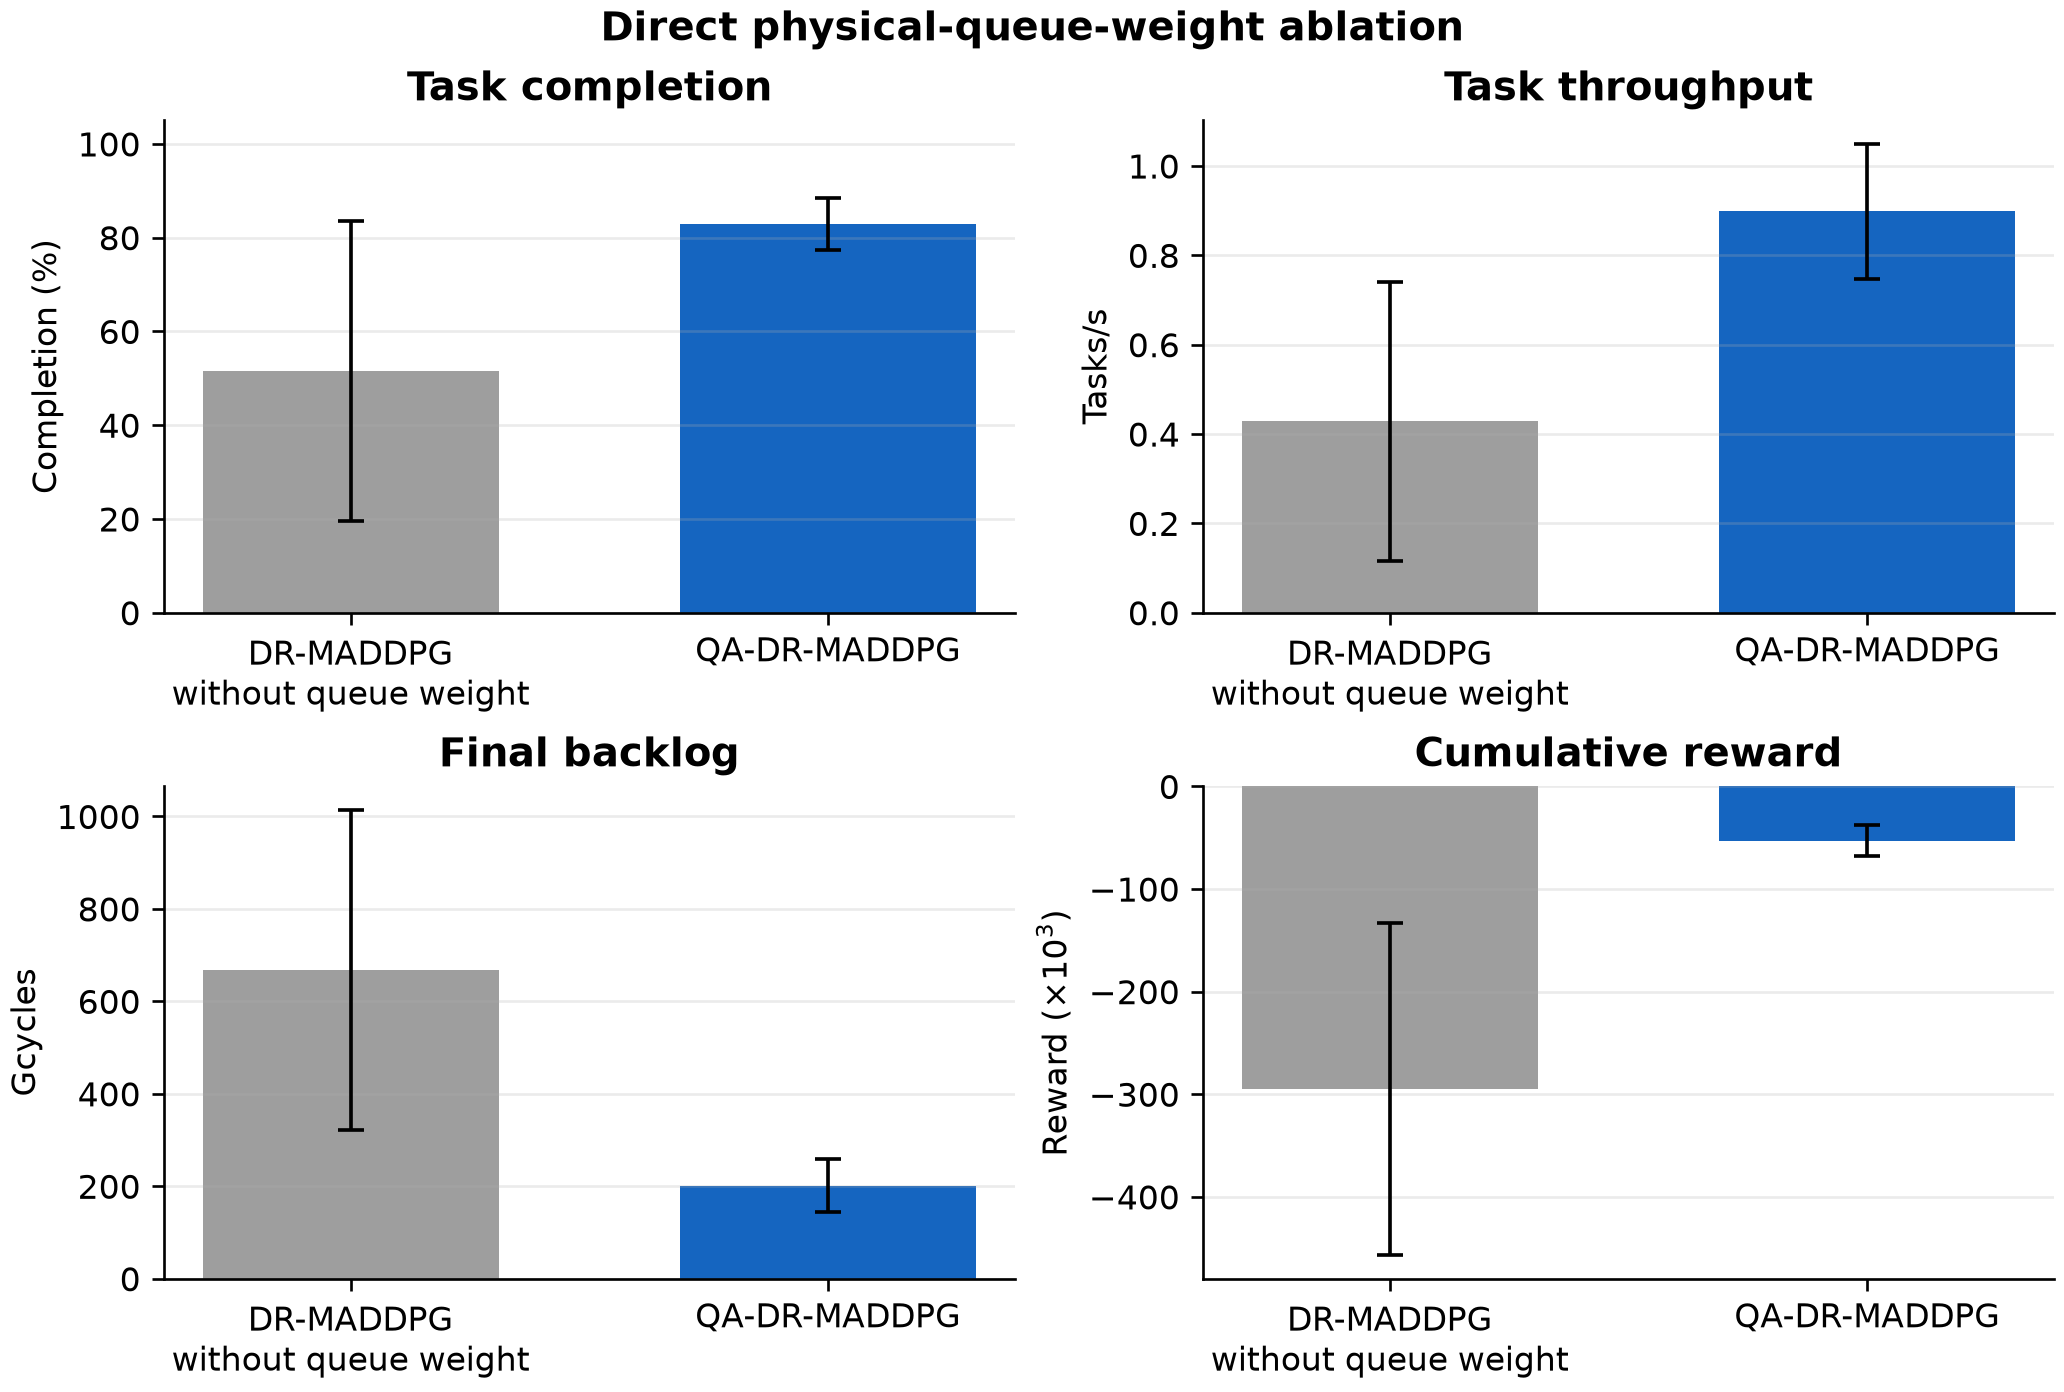
\includegraphics[width=\columnwidth]{queue_weight_ablation.png}
\caption{Direct queue-weight ablation on the domain-randomized MADDPG
backbone. Error bars are 95\% Student-$t$ intervals over five independently
trained learner seeds; the paired-difference intervals are in
Table~\ref{tab:queue_ablation}.}
\label{fig:queue_ablation}
\end{figure}

\subsection{Safety and Decision Latency}
None of the learned methods produced a modeled battery violation, separation
violation or physical-feasibility failure in the frozen test runs. This
result leans heavily on the repair step. Mean repair rates were 100\% for
Hybrid MADDPG and \method, 98.5\% for Reptile-MADDPG, 94.4\% for its no-queue
variant and 95.1\% for MAPPO, which means the modeled safety belongs to the
actor and the feasibility controller together and not to the raw neural
proposal. Mean decision latency was 3.84 ms for Hybrid MADDPG, 3.63 ms for
\method, 2.75 ms for Reptile-MADDPG, 6.44 ms for its no-queue version and
4.47 ms for MAPPO; the corresponding mean 95th-percentile latencies were
5.26, 5.29, 3.35, 9.16 and 8.49 ms.

\subsection{Topology and Capacity Scalability Scope}
The offered-load experiments above all use the same small topology: three
vehicles, two RSUs and two UAVs at static synthetic positions, with fixed
uplink capacities. They do not show that performance carries over to larger
fleets, or that it is insensitive to altitude, coverage or channel changes.
Testing scalability properly would mean varying the numbers of vehicles and
UAVs, the offered load, the backhaul capacity and the harvesting rate, with
either retraining or a topology-compatible masked encoder. Those experiments
have not been run, and we have not filled their place with approximated
values.

\subsection{Interpretation and Limitations}
Three points stand out from these experiments. Training hybrid MADDPG on a
wider set of domains improved its observed service averages. Energy alone is
not a fair performance measure, since a controller can lower it by leaving
UAVs unavailable and tasks unfinished. And because actions were repaired so
often, the measured execution safety still relies on the feasibility layer.

The study also has clear limitations. Vehicle positions are static and
synthetic, and the task and harvest traces are synthetic too. The benchmark
uses fixed uplink capacities in place of the geometry-aware channel. With
five learner seeds, the confidence intervals stay wide. The focused ablation
was run on separately retrained checkpoints, not on those of the full
benchmark. Finally, no online updates were made during evaluation. That
matches the fixed domain-randomized policy we propose, but it also means our
evidence cannot be presented as few-shot adaptation.

\section{Conclusion}
This report introduced \method, a queue-aware, domain-randomized hybrid
MADDPG controller for a multi-UAV vehicular edge--cloud network. The
underlying model covers persistent task stages, radio and computing capacity,
UAV flight and hover energy, harvesting, battery causality, a landing reserve
and collision avoidance. One fixed CTDE policy is trained over seven
operating conditions, and a Lyapunov reward ties the physical and virtual
queues to the service and energy decisions.

On held-out paired scenarios and over five learner seeds, the
domain-randomized controller reached higher numerical deadline success,
completion, throughput and reward than nominal Hybrid MADDPG. It also beat
the current Reptile variant on completion and reward, while Hybrid MAPPO kept
a slightly higher deadline-success rate. In the direct ablation,
physical-queue weighting gave statistically established gains in throughput,
backlog and reward under the five-seed protocol. Every learned method stayed
physically feasible behind the shared safety layer, although the high repair
rates show that the raw actor outputs are not safe by themselves. The next
steps are to train more learner seeds, switch on recorded mobility and
geometry-aware radio service, test sensitivity to topology and parameters,
and adjust the service constraints so that energy-saving policies do not
land UAVs excessively.

\IEEEtriggeratref{10}
\begin{thebibliography}{99}
\bibitem{zhang2019mobile}
S.~Zhang, H.~Zhang, B.~Di, and L.~Song, ``Cellular UAV-to-X communications:
Design and optimization for multi-UAV networks,'' \emph{IEEE Trans. Wireless
Commun.}, vol.~18, no.~2, pp.~1346--1359, 2019.

\bibitem{liu2020uav}
Y.~Liu, K.~Xiong, Q.~Ni, P.~Fan, and K.~B. Letaief, ``UAV-assisted wireless
powered cooperative mobile edge computing: Joint offloading, CPU control, and
trajectory optimization,'' \emph{IEEE Internet Things J.}, vol.~7, no.~4,
pp.~2777--2790, 2020.

\bibitem{neely2010stochastic}
M.~J. Neely, \emph{Stochastic Network Optimization with Application to
Communication and Queueing Systems}. Morgan \& Claypool, 2010.

\bibitem{mao2017dynamic}
Y.~Mao, J.~Zhang, and K.~B. Letaief, ``Dynamic computation offloading for
mobile-edge computing with energy harvesting devices,'' \emph{IEEE J. Sel.
Areas Commun.}, vol.~34, no.~12, pp.~3590--3605, 2016.

\bibitem{sun2026qtop}
H.~Sun, H.~Chen, H.~Xue, L.~Wu, Z.~Li, N.~Chen, W.~Liu, and J.~Yu,
``Q-TOP: Queue-aware task offloading and path planning for multi-UAV assisted
vehicular edge computing networks,'' \emph{IEEE Trans. Veh. Technol.},
accepted manuscript, 2026, doi: 10.1109/TVT.2026.3721145.

\bibitem{lowe2017multi}
R.~Lowe \emph{et al.}, ``Multi-agent actor-critic for mixed cooperative-
competitive environments,'' in \emph{Advances in Neural Information
Processing Systems}, 2017.

\bibitem{schulman2017proximal}
J.~Schulman \emph{et al.}, ``Proximal policy optimization algorithms,''
arXiv:1707.06347, 2017.

\bibitem{talukdar2026mappo}
N.~Talukdar, T.~Barai, A.~Hazra, and N.~Mazumdar, ``MAPPO-driven task quality optimization with
wireless energy transfer in multi-UAV MEC-enabled IoT networks,'' \emph{IEEE
Trans. Sustainable Computing}, vol.~11, no.~3, pp.~302--315, 2026,
doi: 10.1109/TSUSC.2026.3688744.

\bibitem{finn2017model}
C.~Finn, P.~Abbeel, and S.~Levine, ``Model-agnostic meta-learning for fast
adaptation of deep networks,'' in \emph{Proc. ICML}, 2017.

\bibitem{nichol2018reptile}
A.~Nichol, J.~Achiam, and J.~Schulman, ``On first-order meta-learning
algorithms,'' arXiv:1803.02999, 2018.

\bibitem{yan2026rmaddpg}
M.~Yan, P.~Yu, J.~Chen, C.~Li, and C.-L.~I, ``Dynamic computation offloading
optimization based on meta-reinforcement learning in UAV-assisted MEC
networks,'' \emph{IEEE Internet Things J.}, vol.~13, no.~11,
pp.~23615--23627, 2026, doi: 10.1109/JIOT.2026.3670318.

\bibitem{xiong2021energy}
Z.~Xiong \emph{et al.}, ``UAV-assisted wireless energy and data transfer with
deep reinforcement learning,'' \emph{IEEE Trans. Cogn. Commun. Netw.},
vol.~7, no.~1, pp.~85--99, 2021.

\bibitem{guo2024multi}
H.~Guo, Y.~Wang, J.~Liu, and C.~Liu, ``Multi-UAV cooperative task offloading
and resource allocation in 5G advanced and beyond,'' \emph{IEEE Trans.
Wireless Commun.}, vol.~23, no.~1, pp.~347--359, 2024.

\bibitem{liang2025rav}
H.~Liang \emph{et al.}, ``Joint task partitioning and resource allocation in
RAV-enabled vehicular edge computing based on deep reinforcement learning,''
\emph{IEEE Internet Things J.}, vol.~12, no.~11, pp.~15453--15466, 2025.

\bibitem{tang2025dnn}
X.~Tang \emph{et al.}, ``DNN task assignment in UAV networks: A generative
AI enhanced multiagent reinforcement learning approach,'' \emph{IEEE Internet
Things J.}, vol.~12, no.~10, pp.~13340--13352, 2025.

\bibitem{tobin2017domain}
J.~Tobin \emph{et al.}, ``Domain randomization for transferring deep neural
networks from simulation to the real world,'' in \emph{Proc. IEEE/RSJ Int.
Conf. Intell. Robots Syst.}, 2017, pp.~23--30.

\bibitem{peng2018sim}
X.~B. Peng, M.~Andrychowicz, W.~Zaremba, and P.~Abbeel, ``Sim-to-real
transfer of robotic control with dynamics randomization,'' in \emph{Proc.
IEEE Int. Conf. Robot. Autom.}, 2018, pp.~3803--3810.

\bibitem{zhang2019predictive}
Q.~Zhang, M.~Mozaffari, W.~Saad, M.~Bennis, and M.~Debbah, ``Machine learning
for predictive on-demand deployment of UAVs for wireless communications,''
arXiv:1805.00061, 2018.
\end{thebibliography}

\end{document}
